% Official and up-to-date UC Berkeley guidelines on
% dissertation formatting can be found here:
% https://grad.berkeley.edu/academic-progress/dissertation/

%%%%%%%%%%%%%%%%%%%%
%%%%% PACKAGES %%%%%
%%%%%%%%%%%%%%%%%%%%

\documentclass{ucbthesis}
%\usepackage{biblatex}
\usepackage{natbib} % use natbib over biblatex to be able to use GSAB .bst
\usepackage{textcomp,marvosym}
\usepackage{amsmath,amssymb}
\usepackage{rotating}
\usepackage{graphicx}
\usepackage{xspace}
\usepackage[hidelinks]{hyperref}
\urlstyle{same}
\usepackage{threeparttable}
\usepackage[font=footnotesize,format=plain,labelfont=bf,up,textfont=up]{caption} % change figure caption style
\usepackage{color,colortbl}
\usepackage{bibentry}
\bibliographystyle{gsabull}

% To compile this file, run "latex thesis", then "biber thesis"
% (or "bibtex thesis", if the output from latex asks for that instead),
% and then "latex thesis" (without the quotes in each case).

% Double spacing, if you want it. Do not use for the final copy.
% \def\dsp{\def\baselinestretch{2.0}\large\normalsize}
% \dsp

% If the Grad. Division insists that the first paragraph of a section
% be indented (like the others), then include this line:
% \usepackage{indentfirst}

\addtolength{\abovecaptionskip}{\baselineskip}

% Not sure why, but this is required by the style class
\newtheorem{theorem}{Jibberish}

% set hyphenation rules if words are not hyphenated properly
%\hyphenation{mar-gin-al-ia}

%%%%%%%%%%%%%%%%%%%
%%%%% SYMBOLS %%%%%
%%%%%%%%%%%%%%%%%%%

\newcommand{\degreesC}{$^{\circ}$C\xspace}
\newcommand{\degrees}{$^{\circ}$\xspace}
\newcommand{\dC}{$\delta^{13}$C\xspace}
\newcommand{\dO}{$\delta^{18}$O\xspace}
\newcommand{\SrSr}{$^{87}$Sr/$^{86}$Sr\xspace}
\newcommand{\permil}{\textperthousand\xspace}
\newcommand{\dsil}{$d$\xspace}
\newcommand{\UPb}{$^{206}$Pb/$^{238}$U\xspace}
\newcommand{\pCOtwo}{$p$CO$_{2}$\xspace}
\newcommand{\COtwo}{CO$_{2}$\xspace}
\newcommand{\SI}{\textit{Supporting Information}\xspace}
\newcommand{\MM}{\textit{Materials and Methods}\xspace}

\definecolor{Yellow}{rgb}{1,1,0.35}

%%%%%%%%%%%%%%%%%%%%%%%%
%%%%% FRONT MATTER %%%%%
%%%%%%%%%%%%%%%%%%%%%%%%

\begin{document}
\nobibliography* % enigmatically required to use bibentry

\title{Planetary cooling, tectonics, and weathering from 1 billion years ago to the present}

\author{Yuem Park}
\degreesemester{Fall}
\degreeyear{2020}
\degree{Doctor of Philosophy}
\chair{Professor Nicholas L. Swanson-Hysell}
\othermembers{Professor Daniel A. Stolper \\
			  Professor Seth Finnegan}
% For a co-chair who is subordinate to the \chair listed above
% \cochair{Professor Benedict Francis Pope}
% For two co-chairs of equal standing (do not use \chair with this one)
% \cochairs{Professor Richard Francis Sony}{Professor Benedict Francis Pope}
\numberofmembers{3}
\field{Earth \& Planetary Science}
% This is optional (default is Berkeley)
% \campus{Berkeley}

\maketitle
% Delete (or comment out) the \approvalpage line for the final version.
\approvalpage
\copyrightpage

\begin{abstract}

Over the past one billion years, Earth's climate has fluctuated between three stable states on million year time-scales: a warm state in which the poles are ice-free, a cold state in which finite ice caps exist at the poles, and a ``snowball'' state in which Earth's entire surface is covered by ice. Changes in global weatherability could be responsible for driving transitions between these climate states by modulating the atmospheric \COtwo concentration (\pCOtwo) at which \COtwo input from volcanism into Earth's ocean/atmosphere system is removed via silicate weathering. Since the presence of mafic and ultramafic rocks in the warm and wet tropics increases global weatherability, it has both been hypothesized that island arc exhumation and large igneous province eruption at low latitudes have driven cooling on million year time-scales. In the chapters presented in this dissertation, we evaluate these two hypotheses.

In Chapter 1, we reconstruct the paleogeographic position of major arc-continent collisions and large igneous provinces to assess whether a first-order correlation between these two tectonic settings and changes in Earth's climate state can be established for the Phanerozoic. Arc-continent collisions are quantified as the length of sutures that are active at any given time, and large igneous provinces are quantified as the area of surface volcanics remaining following eruption after a parameterization of erosion has been applied. The latitudinal distribution of continental ice sheets is used as a proxy for Earth's climate state. Our analyses reveal a strong correlation between active suture length in the tropics and the extent of glaciation, and no significant correlation between large igneous province area in the tropics and the extent of glaciation. The key difference between large igneous provinces and active orogens involving island arcs is continuous exhumation and the creation of steep topography in the orogens. Therefore, our results suggest that changes in Earth's climate state are primarily driven by island arc exhumation in the tropics due to the combination of mafic and ultramafic lithologies, a warm and wet tropical environment, high erosion rates, and a lack of thick regoliths in this tectonic setting. In contrast, large igneous provinces have low erosion rates and develop thick regoliths, dampening their influence on global weatherability and Earth's climate state.

However, this correlation between arc-continent collisions in the tropics and Earth's climate state over the Phanerozoic does not necessitate causation. The magnitude of decrease in steady-state \pCOtwo associated with specific instances of arc-continent collision in the tropics needs to be quantified. Ongoing arc–continent collision in the tropical Southeast Asian islands has increased the area of subaerially exposed land in the region since the mid-Miocene. Concurrently, Earth’s climate has cooled since the Miocene Climatic Optimum, leading to growth of the Antarctic ice sheet and the onset of Northern Hemisphere glaciation. In Chapter 2, we compile paleoshoreline data and incorporate them into a numerical model that couples a global climate model to a silicate weathering model with spatially resolved lithology. We find that without the increase in area of the Southeast Asian islands over the Neogene, \pCOtwo would have been significantly higher than pre-industrial values, remaining above the levels necessary for initiating Northern Hemisphere ice sheets.

As such, there is accumulating evidence that supports the notion that transitions between ice-free and ice-cap climate states is primarily driven by island arc exhumation in the tropics. However, it remains unclear whether transitions into the snowball climate state are driven by the same mechanism. In Chapter 3, we investigate the Tonian-Cryogenian Tambien Group of northern Ethiopia -- a mixed carbonate-siliciclastic sequence that culminates in glacial deposits associated with the ca. 717--660~Ma Sturtian ``Snowball Earth.'' The presence of intercalated tuffs suitable for high-precision geochronology within the Tambien Group enable temporal constraints on stratigraphic data sets of the interval preceding, and leading into, the Sturtian glaciation. \dC and \SrSr data and U-Pb chemical abrasion isotope dilution thermal ionization mass spectrometry (CA-ID-TIMS) ages from the Tambien Group are used in conjunction with previously published isotopic and geochronologic data to construct newly time-calibrated composite Tonian carbon and strontium isotope curves. Tambien Group \dC data and U-Pb CA-ID-TIMS ages reveal that a pre-Sturtian sharp negative \dC excursion precedes the Sturtian glaciation by $\sim$18~Myr and is followed by a prolonged interval of positive \dC values, suggesting that perturbations to the carbon cycle that lead to sharp negative \dC excursions are unrelated to the initiation of the Sturtian glaciation. The composite Tonian \SrSr curve shows that, following an extended interval of low and relatively invariant values, inferred seawater \SrSr rose ca. 880--770~Ma, and then decreased to the ca. 717~Ma initiation of the Sturtian glaciation. These data, when combined with a simple global weathering model and analyses of the timing and paleolatitude of large igneous province eruptions and island arc exhumation events, suggest that the \SrSr increase was influenced by increased subaerial weathering of radiogenic lithologies as the (super)continent Rodinia rifted apart at low latitudes. The following \SrSr decrease is consistent with enhanced subaerial weathering of island arc lithologies accreting in the tropics over tens of millions of years, lowering \pCOtwo and contributing to the initiation of the Sturtian glaciation.

However, a lack of paleomagnetic data to constrain the paleolatitude and configuration of tectonic blocks during the Tonian hampers efforts to quantify changes in global weatherability during the lead up to the Sturtian glaciation. South China is associated with arc-continent collisions during the Tonian, and is at the center of debates regarding the configuration of Rodinia, with competing models variably placing the block at the core or periphery of Rodinia, or separated from it entirely. Tonian paleogeographic models also vary in whether they incorporate proposed large and rapid oscillatory true polar wander associated with the ca. 810--795~Ma Bitter Springs Stage. In Chapter 4, we develop new paleomagnetic data paired with U-Pb CA-ID-TIMS geochronology from the Tonian Xiajiang Group in South China to establish the block's position and test the Bitter Springs Stage true polar wander hypothesis. The data constrain South China to high latitudes ca. 813~Ma, and when considered in conjunction with other paleomagnetic poles from South China, indicate a relatively stable high-latitude position ca. 821--805~Ma. The difference in pole position between the pre-Bitter Springs Stage Xiajiang Group pole and the syn-Bitter Springs Stage Madiyi Formation pole is significantly less than that predicted for the Bitter Springs Stage true polar wander hypothesis. These constraints place the craton at higher latitudes connected to Rodinia along its periphery, or disconnected from Rodinia entirely. If this pole difference is interpreted as true polar wander superimposed upon differential plate motion, it requires South China to have been separate from Rodinia.

Put together, we find that the exhumation of island arcs and oceanic crust during arc-continent collision and arc-accretion events in the tropics are important for driving shifts in Earth's climate state over the past one billion years.

\end{abstract}


\begin{frontmatter}

%%%%%%%%%%%%%%%%%%%%%%%%%
%%%%% TOC AND LISTS %%%%%
%%%%%%%%%%%%%%%%%%%%%%%%%

\tableofcontents
\clearpage
\listoffigures
\clearpage
\listoftables

%%%%%%%%%%%%%%%%%%%
%%%%% PREFACE %%%%%
%%%%%%%%%%%%%%%%%%%

\begin{preface}
\phantomsection % make the ToC links work
\addcontentsline{toc}{chapter}{Preface} % add to ToC

The material within the chapters of this dissertation are largely taken from previously published (or soon to be published) articles. The following text identifies these articles, and provides some additional context about how they relate to one another.

\subsubsection*{Chapter 1 - Evaluating the relationship between the area and latitude of large igneous provinces and Earth's long-term climate state}

\noindent
\bibentry{Macdonald2019a}

\medskip

\noindent
\bibentry{Park2019a}

\bigskip

In \citet{Macdonald2019a}, I developed a workflow built on pyGPlates (software for the analysis of paleogeographic models) that allowed us to calculate the area/length of paleogeographically reconstructed polygons/lines within different latitude bands through time. By pairing this workflow with a database of ophiolite-bearing sutures and a paleogeographic model, we were able to identify a strong correlation between arc-continent collisions in the tropics (measured as active suture length in the tropics) and times of glacial climate over the past $\sim$520~m.y. This correlation led to our proposal that Earth's climate state is set primarily by global weatherability, which changes with the latitudinal distribution of arc-continent collisions. Similarly, it has been proposed elsewhere that the eruption/drift of large igneous provinces into the tropics has driven global cooling. The pyGPlates workflow that I developed provided a means through which we could evaluate this hypothesis. \citet{Park2019a} builds upon the zonal large igneous province area analysis that I conducted and presented in the supplementary materials for \citet{Macdonald2019a} by more rigorously developing parameterizations of large igneous province erosion and exploring several geologically reasonable large igneous province post-emplacement scenarios.

\citet{Park2019a} is currently available as a preprint on EarthArXiv, but a slightly modified version of the article is scheduled to be formally published within 2020 as Chapter 7 of AGU Geophysical Monograph Series 255, titled \textit{Large Igneous Provinces: A Driver of Global Environmental and Biotic Changes}, edited by Richard E. Ernst, Alexander J. Dickson, and Andrey Bekker.

Code used to perform the analyses presented in these articles are available on GitHub at \url{https://github.com/Swanson-Hysell-Group/Arc_Continent_Analysis} and \url{https://github.com/Swanson-Hysell-Group/2020_large_igneous_provinces}, or on Zenodo at \url{https://doi.org/10.5281/zenodo.2636731} and \url{https://doi.org/10.5281/zenodo.3981262}.

\subsubsection*{Chapter 2 - Emergence of the Southeast Asian islands as a driver for Neogene cooling}

\noindent
\bibentry{Park2020b}

\bigskip

This article was the result of a collaboration between Godd\'eris' and Swanson-Hysell's research groups supported by the France-Berkeley Fund. Broadly speaking, the collaboration was intended to investigate whether numerical Earth system models quantitatively support the hypothesis put forward in \citet{Macdonald2019a} and \citet{Swanson-Hysell2017a} that tropical arc-continent collisions set Earth's climate state. The model that we use is the global spatially resolved GEOCLIM model, which estimates changes in steady-state \pCOtwo associated with coupled changes in erosion, chemical weathering, and climatology by linking a silicate weathering model to climate model runs at multiple \pCOtwo levels. In previous versions of the model, Godd\'eris and his collaborators parameterized silicate weathering to be a function of temperature and runoff only, and all bedrock was assigned identical chemical compositions. In a more recent version of the model, Maffre implemented regolith development and soil shielding, which introduced a dependence on erosion rate (and, therefore, topographic slope). While this introduction of regolith development into GEOCLIM is important for assessing the impact of tropical arc–continent collisions on \pCOtwo, the relatively high Ca+Mg concentration in arc rocks relative to other lithologies must also be considered. Therefore, in \citet{Park2020b}, I implemented variable bedrock Ca+Mg concentration into GEOCLIM and quantified the uncertainty in steady-state \pCOtwo that arises from poorly constrained model parameters.

The code for the GEOCLIM model used in this study can be found at \url{https://github.com/piermafrost/GEOCLIM-dynsoil-steady-state/releases/tag/v1.0}. The code that generated the inputs and analyzed the output of the GEOCLIM model can be found at \url{https://github.com/Swanson-Hysell-Group/2020_Southeast_Asian_Islands} or \url{https://doi.org/10.5281/zenodo.4021653}.

\subsubsection*{Chapter 3 - The lead-up to the Sturtian Snowball Earth: Neoproterozoic chemostratigraphy time-calibrated by the Tambien Group of Ethiopia}

\noindent
\bibentry{MacLennan2018a}

\medskip

\noindent
\bibentry{Park2020a}

\bigskip

Chronologically, the work that lead to \citet{MacLennan2018a} and \citet{Park2020a} largely preceded the projects presented in Chapters 1 and 2. In \citet{MacLennan2018a}, we presented the initial geochronologic results that placed temporal constraints on large excursions in the marine \dC record and the initiation of the Sturtian glaciation in a short-format journal. \citet{Park2020a} built upon this work by: thoroughly documenting the geology of the Tambien Group in northern Ethiopia (including the discovery of vast areas of exposures of Sturtian glacial deposits and underlying strata near the town of Samre), presenting additional geochronologic results, assessing diagenesis in carbonate samples, presenting the complete \dC and \SrSr data from the Tambien Group, developing a composite Tonian-Cryogenian \dC and \SrSr chemostratigraphic record, and proposing a model for the initiation of the Sturtian glaciation based on the composite \SrSr chemostratigraphic record, a simple global weathering model, and analyses of the timing and paleolatitude of large igneous province eruptions and arc accretion events. As in \citet{Swanson-Hysell2017a} and \citet{Macdonald2019a}, the model for the initiation of the Sturtian glaciation proposed in \citet{Park2020a} called upon island arc exhumation in the tropics, and was part of the motivation to initiate a collaboration with Godd\'eris' research group.

Code used to perform the analyses presented in these articles is available on GitHub at \url{https://github.com/Swanson-Hysell-Group/2019_Tambien_Group}, or on Zenodo at \url{https://doi.org/10.5281/zenodo.3403180}.

\subsubsection*{Chapter 4 - Tonian paleomagnetism from South China permits an inclusive Rodinia or Bitter Springs Stage true polar wander, but not both}

\noindent
\textit{PRE-PRINT CITATION WILL GO HERE}
%\bibentry{Park2020c}

\bigskip

Although \citet{Park2020a} called upon island arc exhumation in the tropics as a critical tectonic boundary condition that allowed for the Sturtian glaciation to take place, a lack of paleomagnetic data to constrain the paleolatitude and configuration of tectonic blocks during the Tonian hampers efforts to quantify changes in global weatherability associated with island arc exhumation during the lead up to the Sturtian glaciation. \citet{Park2020c} develops paleomagnetic data to better constrain the location of one of these tectonic blocks, South China, in the Tonian. South China is a particularly important block to investigate with paleomagnetic data in the context of the Sturtian glaciation because arc-continent collisions are hypothesized to have occurred both within and along the margin of the block during the Tonian. Furthermore, sediments from which paleomagnetic data can be developed exist in South China that span a hypothesized major global tectonic event (Bitter Springs Stage true polar wander) that, if real, has far-reaching implications for the paleogeography of the time.

\citet{Park2020c} is currently available as a preprint on EarthArXiv, and has been submitted to the \textit{Journal of Geophysical Research: Solid Earth} for review.

Code used to perform the analyses presented in these articles is available on GitHub at \url{xxx}, or on Zenodo at \url{xxx}.

\end{preface}

%%%%%%%%%%%%%%%%%%%%%%%%%%%%
%%%%% ACKNOWLEDGEMENTS %%%%%
%%%%%%%%%%%%%%%%%%%%%%%%%%%%

\begin{acknowledgements}
\phantomsection % make the ToC links work
\addcontentsline{toc}{chapter}{Acknowledgements} % add to ToC

None of what is presented in this dissertation would have been possible without the support of innumerable people. It would be impossible to list every one of these people here, but nevertheless I note some of the individuals who were key to making the research possible below.

I sincerely appreciate the expert guidance and advice from the professors with whom I worked to push the research forward throughout the years: Mulugeta Alene, Dan Condon, Seth Finnegan, Yves Godd\'eris, Bereket Haileab, Oli Jagoutz, Lorraine Lisiecki, Francis Macdonald, Adam Maloof, Blair Schoene, Daniel Stolper, and Shihong Zhang.

I thank my graduate student and post-doc collaborators, the Swanson-Hysell Group, and my Ph.D. class, not only for discussing research with me, but also for being great friends: Eliel Anttila, Maggie Avery, Alex Charn, Luke Fairchild, Isabel Fendley, Hairuo Fu, Mulubrhan Gebreslassie, Blake Hodgin, Taylor Kilian, Jinsol Kim, Tanis Leonhardi, Nate Lindsey, Scott MacLennan, Pierre Maffre, Alex Robson, Allison Sharrar, Sarah Slotznick, Tadele Tesema, Marissa Tremblay, Hanbiao Xian, and Yiming Zhang.

I thank the EPS staff for dealing with the logistics of research and being a graduate student: Rachel Kowalik and Margie Winn.

And of course a big thank you to the rest of the undergraduate students, graduate students, post-docs, staff, and faculty in the Department of Earth \& Planetary Science at UC Berkeley and elsewhere, who I didn't have the chance to list here.

In terms of the non-Earth Science people in my life, I thank my friends and my partner Yudith Dian for putting up with me through the years. And of course a huge thank you to my family, who dedicated everything to raising me and getting me to where I am today.

Finally, and most importantly, thank you to my advisor Nick Swanson-Hysell, for accepting me into the program to begin with and then tirelessly mentoring me throughout the years. I'm endlessly appreciative that I was able to work with him and learn from him, and honestly I don't think I could have asked for a better advisor. As his first graduating Ph.D. student, I hope that I didn't set the bar too low for those to follow.

\end{acknowledgements}

\end{frontmatter}

%%%%%%%%%%%%%%%%%%%%
%%%%% CHAPTERS %%%%%
%%%%%%%%%%%%%%%%%%%%

\pagestyle{headings}

% (Optional) \part{First Part}

\include{chap-LIPs}
\chapter[Emergence of the Southeast Asian islands as a driver for Neogene cooling][Southeast Asian islands]{Emergence of the Southeast Asian islands as a driver for Neogene cooling}

\section{Abstract}

Steep topography, a tropical climate, and mafic lithologies contribute to efficient chemical weathering and carbon sequestration in the Southeast Asian islands. Ongoing arc-continent collision between the Sunda-Banda arc system and Australia has increased the area of subaerially exposed land in the region since the mid-Miocene. Concurrently, Earth's climate has cooled since the Miocene Climatic Optimum, leading to growth of the Antarctic ice sheet and onset of Northern Hemisphere glaciation. We seek to evaluate the hypothesis that the emergence of the Southeast Asian islands played a significant role in driving this cooling trend through increasing global weatherability. To do so, we have compiled paleoshoreline data and incorporated them into GEOCLIM, which couples a global climate model to a silicate weathering model with spatially resolved lithology. We find that without the increase in area of the Southeast Asian islands over the Neogene, atmospheric \pCOtwo would have been significantly higher than pre-industrial values, remaining above the levels necessary for initiating Northern Hemisphere ice sheets.

\section{Introduction}

The Southeast Asian islands (SEAIs) have an out-sized contribution to modern chemical weathering fluxes relative to its area. The confluence of steep topography, a warm and wet tropical climate, and the presence of mafic lithologies results in high fluxes of Ca and Mg cations in the dissolved load and associated \COtwo consumption \citep{Gaillardet1999a, Hartmann2009a, Milliman2013a, Hartmann2014a}. There has been a significant increase in the area of subaerially exposed land within the region since the mid-Miocene associated with ongoing arc-continent collision between Australia and the Sunda-Banda arc system \citep{Molnar2015a, Hall2017a, Macdonald2019a}. Concurrently, after the Miocene Climatic Optimum, a cooling trend began ca. 15~Ma and accelerated over the past 4 million years (m.y.) leading to the development of Northern Hemisphere ice sheets \citep{Shackleton1984a, Zachos2001a}. Many hypotheses have been proposed to explain this cooling trend including changes in ocean/atmosphere circulation \citep{Haug1998a, Shevenell2004a, Molnar2015a}, a decrease in volcanic degassing \citep{Berner1983a}, or uplift in the Himalaya \citep{Raymo1988a, Galy2007a}. Here we seek to evaluate the hypothesis that emergence of the SEAIs was a significant factor in driving long-term climatic cooling over the Neogene.

Over geologic time-scales, \COtwo enters Earth's ocean--atmosphere system primarily via volcanism and metamorphic degassing, and leaves primarily through the chemical weathering of silicate rocks and through organic carbon burial \citep{Kump2000a}. Chemical weathering delivers alkalinity and cations to the ocean which drives carbon sequestration through carbonate precipitation. Steady-state \pCOtwo is set at the \pCOtwo level at which \COtwo sinks are equal to sources. As \COtwo sinks increase and \pCOtwo falls, temperature decreases and the hydrological cycle is weakened, causing the efficiency of the silicate weathering sink to decrease until a new steady-state is achieved at lower \pCOtwo \citep{Kump1997a}.

Topography, climate, and lithology all effect chemical weathering. High-relief regions generally lack extensive regolith development, and thus tend to have reaction-limited weathering regimes that are more prone to adjust when climate changes \citep{Gabet2009a, West2012a, Maher2014a}. High physical erosion rates contribute to high chemical weathering fluxes in these high-relief regions \citep{Godderis2017b}. In warm and wet regions, mineral dissolution kinetics are faster leading to enhanced chemical weathering \citep{Lasaga1994a, West2012a}. Mafic rocks have higher Ca and Mg concentrations and dissolution rates than felsic rocks, and thus have the potential to more efficiently sequester carbon through silicate weathering \citep{Dessert2003a}. These factors have led to the proposal that arc-continent collisions, which create steep landscapes that include mafic lithologies, within the tropical rain belt have been important in enhancing global weatherability, lowering atmospheric \pCOtwo, and initiating glacial climate over the past 520~m.y. \citep{Jagoutz2016a, Swanson-Hysell2017a, Macdonald2019a} and perhaps in the Neoproterozoic as well \citep{Park2020a}.

Quantitatively estimating the magnitude of decrease in steady-state \pCOtwo associated with the emergence of a region with a high carbon sequestration potential, such as the SEAIs, requires constraints on changing tectonic context and accounting of associated feedbacks. As this region emerges, the total global silicate weathering flux will transiently exceed the volcanic degassing flux, causing \pCOtwo to initially decline until a new steady-state is established where the total magnitude of the \COtwo sinks is the same as before the change. However, the sensitivity of the silicate weathering flux in any particular location to this change in \pCOtwo is variable and dependent on the specific topography, climate, and lithology at that location. Furthermore, how regional climate responds to this change in \pCOtwo is itself spatially variable. Therefore, the magnitude of \pCOtwo change that is required to balance the total global silicate weathering flux with the volcanic degassing flux will depend on the specific spatial distribution of topography, climate, and lithology at the time of emergence. As a result, any attempt to meaningfully estimate the decrease in steady-state \pCOtwo associated with emergence of the SEAIs must model spatially resolved climatology and silicate weathering fluxes in tandem and account for the spatial distribution of the factors that affect these inter-connected systems.

\section{GEOCLIM Model}

To estimate the decrease in steady-state \pCOtwo associated with the increase of subaerially exposed land area in the SEAIs, we use the global spatially resolved GEOCLIM model \citep{Godderis2017c}. GEOCLIM estimates changes in steady-state \pCOtwo associated with coupled changes in erosion, chemical weathering, and climatology by linking a silicate weathering model to climate model runs at multiple \pCOtwo levels.

\begin{figure}[h!]
\begin{center}
	\includegraphics[width=0.5\textwidth]{figures/SEAIs/regolith-schematic.pdf}
	\caption[Schematic representation of the silicate weathering component of GEOCLIM.]{A schematic representation of the silicate weathering component of GEOCLIM in a single profile at steady-state. A rock particle leaves the unweathered bedrock with production rate $P_{r}$, and transits vertically through a regolith of height $h$. Regolith production and physical erosion ($E_{p}$) are equal at steady-state. As a particle transits upwards, some fraction of the primary phases ($x$) are chemically weathered ($W$), with the flux of dissolved Ca+Mg being $W$ multiplied by the concentration of Ca+Mg in unweathered bedrock ($\chi_{CaMg}$). Details of the formulation for the silicate weathering component of GEOCLIM can be found in \MM.}
	\label{fig:regolith-schematic}
\end{center}
\end{figure}

The silicate weathering component of GEOCLIM calculates \COtwo consumption resulting from silicate weathering for subaerially exposed land. We assume that Ca and Mg are the only cations that consume \COtwo over geologic time-scales, such that each mole of Ca or Mg that is dissolved by silicate weathering consumes one mole of \COtwo. While reverse weathering is another potential sink for Ca or Mg \citep{Michalopoulos1995a}, its parameterization is unclear and it has been interpreted to be a relatively minor flux in the Cenozoic \citep{Isson2018a}, and we do not include it in our model. In previous versions of the model, silicate weathering was a function of temperature and runoff only, and all bedrock was assigned identical chemical compositions \citep{Godderis2017c}. More recent versions of GEOCLIM implement regolith development and soil shielding (Fig. \ref{fig:regolith-schematic}), which introduces a dependence on erosion rate (and therefore topographic slope; \citealp{Maffre2018a}). While this introduction of regolith development into GEOCLIM is important for assessing the impact of tropical arc-continent collisions on \pCOtwo, the relatively high Ca+Mg concentration in arc rocks relative to other lithologies must also be considered.

We therefore implement variable bedrock Ca+Mg concentration into GEOCLIM (\SI). The spatial distribution of lithologies is sourced from the Global Lithologic Map (GLiM; \citealp{Hartmann2012a}) and is represented by 6 categories: metamorphic, felsic, intermediate, mafic, carbonate, and siliciclastic sediment. Each land pixel is assigned these lithologic categories at a resolution of 0.1\degrees $\times$ 0.1\degrees. The Ca+Mg concentrations of felsic, intermediate, and mafic lithologies are assigned based on the mean of data of these lithologic categories compiled in EarthChem (\url{www.earthchem.org/portal}). Given that GLiM does not distinguish ultramafic lithologies, such rocks are grouped with mafic rocks. As a result, the Ca+Mg concentration is likely an underestimate in regions of obducted ophiolites, such that the estimated effect of these regions on changing steady-state \pCOtwo could be conservative \citep{Schopka2011a}. The weathering of carbonate does not contribute to long-term \COtwo consumption and its Ca+Mg concentration is ignored. The Ca+Mg concentrations of metamorphic and siliciclastic sediment lithologies are more difficult to define, since their chemical composition is strongly dependent on protolith composition and, in the case of siliciclastic sediment, the degree of previous chemical depletion. We explore a range of feasible Ca+Mg concentrations for metamorphic rocks and siliciclastic sediment during calibration of the silicate weathering component of GEOCLIM.

\subsection{Calibration}

The values of four parameters within the silicate weathering component that modify the dependence of silicate weathering on temperature, runoff, erosion, and regolith thickness are poorly constrained. Rather than prescribing single values, we select multiple values for each of these four parameters along with the Ca+Mg concentration of metamorphic and siliciclastic lithologies from within reasonable ranges (\SI; Table \ref{tab:parameter-combinations}). We then permute all possible combinations of these values for the six parameters, leading to 93,600 unique parameter combinations (i.e. permutations). For each combination, we compute spatially resolved long-term \COtwo consumption associated with Ca+Mg fluxes using present-day runoff, temperature, and slope. We sum computed \COtwo consumption over watersheds for which data-constrained estimates are available \citep{Gaillardet1999a, Moquet2018a}, then calculate the coefficient of determination ($r^{2}$) between computed and measured \COtwo consumption in each of these watersheds. After eliminating parameter combinations that result in low $r^{2}$, 573 parameter combinations remain (\SI; Fig. \ref{fig:W-vs-r2}). The resulting global \COtwo consumption of these filtered model runs all overlap with independently derived estimates of the global \COtwo degassing flux \citep{Gerlach2011a}, as they should for a steady-state long-term carbon cycle (\SI; Fig. \ref{fig:W-vs-r2}).

\subsection{Climate Model Component}

Having calibrated the silicate weathering component of GEOCLIM, we use it to estimate the decrease in steady-state \pCOtwo associated with emergence of the SEAIs. For the climate model component, we use temperature and runoff from a subset of the GFDL CM2.0 experiments (\SI; \citealp{Delworth2006b}). These experiments are well-suited for this analysis because all non-\COtwo forcings are held constant at values representative of pre-industrial conditions, allowing the effect of changing \pCOtwo on climatology to be isolated. Furthermore, the experiments were run long enough for the final system to approximate steady-state.

\section{Paleoshorelines}

\begin{figure}[h!]
\begin{center}
	\includegraphics[width=0.9\textwidth]{figures/SEAIs/shoreline-growth.pdf}
	\caption[Emergence of the Southeast Asian islands from the mid-Miocene to present.]{The emergence of the Southeast Asian islands (also referred to as the Maritime Continent in the climate science literature) from the mid-Miocene to present. Past shorelines at 5, 10, and 15 Ma are shown in \textbf{A} with associated land area summarized in \textbf{B}. A significant increase in area over the past 5 million years is coincident with cooling and the onset of Northern Hemisphere glaciation as reflected in the benthic oxygen isotope record \citep{Zachos2008a} shown in \textbf{C}.}
	\label{fig:shoreline-growth}
\end{center}
\end{figure}

\begin{figure}[h!]
\begin{center}
	\includegraphics[width=\textwidth]{figures/SEAIs/scenario-pCO2.pdf}
	\caption[Steady-state \pCOtwo estimates from GEOCLIM.]{Steady-state \pCOtwo estimates from GEOCLIM for the various scenarios discussed in the text. For each of the seven scenarios, each point represents an estimate from one of the 573 unique parameter combinations that most closely matched estimates of present-day \COtwo consumption in 80 watersheds around the world (\SI). The box encloses the middle 50\% of the \pCOtwo estimates (i.e. the interquartile range), and the notch represents the median with its 95\% confidence interval. The whiskers extend to the 2.5 and 97.5 percentile values. Glaciation thresholds \citep{DeConto2008a} are shown on the x-axis.}
	\label{fig:scenario-pCO2}
\end{center}
\end{figure}

To determine the position of paleoshorelines in the SEAIs over the past 15~m.y., we use terrestrial and marine sedimentary deposits (Fig. \ref{fig:shoreline-growth}; \SI). The paleoshoreline data indicate that the Sunda-Banda Arc and New Guinea are primarily responsible for the increase in area since 15~Ma. Exhumation of the modern Sunda-Banda Arc is the result of ongoing arc-continent collision with the Australian Plate \citep{Harris2006a}. Most of Sumatra and Java along with the non-volcanic islands of the Outer Banda Arc were elevated above sea level after 5~Ma \citep{Hall2013b}. In New Guinea, emergence in the mid-Miocene is associated with collision between the Melanesian Arc and Australia's distal margin \citep{Cloos2005a}, which drove exhumation of the Irian-Marum-April Ophiolite Belt. Exhumation accelerated over the past 4~m.y. in the New Guinea Central Range due to slab-breakoff and buoyant uplift, and in eastern New Guinea due to jamming of the north-dipping subduction zone \citep{Cloos2005a}. We also include changes in areas of presently submerged continental shelves such as the Sunda Shelf that were previously exposed (\SI; Fig. \ref{fig:SEAI-fracs}). These tectonic drivers and others throughout the region led to progressive emergence over the past 15~m.y. that accelerated following 5~Ma (Fig. \ref{fig:shoreline-growth}B). This trend mirrors broad cooling over the Neogene that resulted in the initiation of Northern Hemisphere ice sheets (Fig. \ref{fig:shoreline-growth}C).

We use GEOCLIM to estimate \pCOtwo associated with the reconstructed subaerial extent of the SEAIs at ca. 15, 10, and 5~Ma (``paleo-SEAIs'' scenarios; Fig. \ref{fig:scenario-pCO2}). Because we use a climate model forced with modern geography, the position of the tectonic blocks remain fixed. Although there has been motion of these tectonic blocks since 15~Ma, they have remained within tropical latitudes such that this fixed scenario is a good approximation of the paleogeography (\SI; Fig. \ref{fig:paleogeographic-reconstructions}). We also test an end-member scenario, in which all islands associated with arc-continent collision in the region are removed (``removed SEAIs'' scenario; Fig. \ref{fig:scenario-pCO2}).

\section{\pCOtwo Estimates}

Using the 573 unique parameter combinations, the paleo-SEAIs scenarios resulted in 526--678~ppm for 15~Ma, 457--516~ppm for 10~Ma, and 391--434~ppm \pCOtwo for 5~Ma (Fig. \ref{fig:scenario-pCO2}). These results indicate a progressive decrease in \pCOtwo over the Neogene associated with the emergence of the SEAIs, and suggest that without this emergence, pre-industrial \pCOtwo would have been $\sim$526--678~ppm. These paleo-SEAIs scenarios do not account for Neogene changes outside of the SEAIs (e.g. changes in ocean/atmosphere circulation, volcanic degassing, and weathering fluxes elsewhere on Earth, discussed in \textit{Alternative Mechanisms for Neogene Cooling}). Therefore, these results are not estimating \pCOtwo at 15~Ma, but rather are quantifying \pCOtwo change associated with emergence of the SEAIs.

Proxy-based estimates of the magnitude and trajectory of \pCOtwo change from the Miocene to the Pliocene are variable between techniques and associated assumptions underlying their interpretation (\SI; Fig. \ref{fig:pCO2-proxies}). The \pCOtwo values from the 5~Ma paleo-SEAIs scenario overlap with many proxy-based estimates \citep{Foster2017a} as well as values that emerge from approaches that assimilate climate and ice sheet model output with benthic \dO data \citep{van-de-Wal2011a, Berends2020a}. The modeled \pCOtwo values for 15~Ma resemble the higher end of proxy-based \pCOtwo estimates for the early to mid-Miocene, indicating that the increase in subaerially exposed land area and tectonic topography of the SEAIs is sufficient to explain long-term cooling of Earth's climate over the Neogene. The \pCOtwo threshold for Antarctic glaciation is estimated to be $\sim$750~ppm with that for Northern Hemisphere glaciation being significantly lower at $\sim$280~ppm \citep{DeConto2008a}. These modeled values of decreasing \pCOtwo associated with emergence of the SEAIs are therefore consistent with the record of Neogene climate with Miocene ice sheets on Antarctica \citep{Sugden1995a} followed by Northern Hemisphere ice sheets developing in the Pliocene \citep{Haug2005a} as \pCOtwo subsequently decreased.

The results of our paleo-SEAIs scenarios highlight the importance of the combination of topography, runoff, and lithology in setting Earth's climate state. To independently explore the effect of the modern-day surface exposure of lower-relief basaltic lavas on steady-state \pCOtwo \citep{Kent2013a}, we replace mafic volcanics associated with the Deccan Traps, Ethiopian Traps, and Columbia River Basalts with the Ca+Mg concentration of bulk continental crust in GEOCLIM (Fig. \ref{fig:scenario-pCO2}). The resulting \pCOtwo is $\sim$300--500~ppm, indicating that the presence of mafic rocks in these igneous provinces affects steady-state \pCOtwo as has been suggested to be important for Paleogene cooling \citep{Kent2013a}. However, the higher 526--678~ppm values for the 15~Ma paleo-SEAIs scenario illustrate that higher relief and a wet tropical climate significantly increase the efficiency of \COtwo consumption, especially when paired with high Ca+Mg lithologies. As such, arc-continent collisions in the tropics are likely more important for driving long-term changes in \pCOtwo than the eruption of flood basalts \citep{Macdonald2019a, Park2019a}.

Previous work has estimated that the decrease in \pCOtwo since 5~Ma associated with the emergence of the SEAIs and enhanced silicate weathering is $\sim$19~ppm \citep{Molnar2015a}, in which case their emergence would be a relatively minor contributor to Neogene cooling. This 19~ppm estimate was obtained using an equation that assumes a direct linear relationship between mean global temperature and changes in weathering-rate-weighted land area, scaled by a factor that is intended to account for the influence of both runoff and temperature. \pCOtwo was then estimated from the calculated temperature using a simple energy balance equation. However, the relationship between mean global temperature (or \pCOtwo) and weathering-rate-weighted land area is not linear. Furthermore, this simple linear relationship ignores spatial variability in topography and climatology, and only crudely accounts for spatial variability in lithology. In fact, the 19~ppm estimate is closer in magnitude to the decrease in \pCOtwo that we estimate if mafic volcanics associated with the Deccan Traps (a relatively flat area outside of the warm and wet tropics) are replaced with the Ca+Mg concentration of bulk continental crust (22--70 ppm; Fig. \ref{fig:scenario-pCO2}). The significant difference in steady-state \pCOtwo estimated between the ``removed Deccan Traps'' scenario and the paleo-SEAIs scenarios (Fig. \ref{fig:scenario-pCO2}) demonstrates that considering changes in the spatial distribution of lithologies alone is not adequate for estimating changes in steady-state \pCOtwo. Instead, spatially varying topography and climatology significantly modulates silicate weathering rates, and must be accounted for when estimating \pCOtwo change associated with paleogeographic change.

An important caveat for these estimates of \pCOtwo is that our modeling is determining the climatology in the GFDL CM2.0 model at which steady-state is achieved -- a climatology that has an associated \pCOtwo value in the model. However, climate models are variable in their response to changes in \pCOtwo. One way to summarize this variability is through the equilibrium climate sensitivity value -- the steady-state change in global mean surface air temperature associated with a doubling of \pCOtwo. A range of 1.5 to 4.5\degreesC per \pCOtwo doubling was proposed in the landmark Charney report \citep{Charney1979a} and this range was considered to be the credible interval (\textgreater66\% likelihood) in the last IPCC report \citep{Stocker2013a}. Integrating constraints both from understanding of climate feedback processes and the climate record, a recent comprehensive review estimates the 66\% probability range of climate sensitivity to be 2.6 to 3.9\degreesC per \pCOtwo doubling with a 5 to 95\% range of 2.3 to 4.7\degreesC per \pCOtwo doubling \citep{Sherwood2020a}. The equilibrium climate sensitivity associated with the CM2.0 climate models is 2.9\degreesC per \pCOtwo doubling, which falls within these ranges although these ranges remain broad. An alternative way to consider the results from our analysis would be that an estimate of 572~ppm (2$\times$ pre-industrial \pCOtwo) for the 15~Ma paleo-SEAIs scenario is implying that Earth would be $\sim$2.9\degreesC warmer. If Earth's climate sensitivity is at the higher end of the probable range and higher than in the CM2.0 model, as it is in some climate models, this same amount of Neogene cooling resulting from the emergence of the SEAIs could have been driven by a smaller change in \pCOtwo.

\section{Alternative Mechanisms for Neogene Cooling}

\subsection{Ocean/Atmosphere Circulation}

Some hypotheses to explain ice sheet growth over the Neogene invoke changes in ocean/atmosphere circulation including: further climatic isolation of Antarctica due to strengthening of the circumpolar current \citep{Shevenell2004a}; increased atmospheric moisture in the Northern Hemisphere due to intensified thermohaline circulation following Panama Isthmus emergence \citep{Haug1998a}; and cooling of North America resulting from a strengthened Walker Circulation associated with emergence of the SEAIs \citep{Molnar2015a}. Such changes in ocean/atmosphere circulation are likely to modulate \pCOtwo thresholds for glacial initiation and ice sheet growth \citep{DeConto2008a}. However, the prolonged time-scale of the cooling trend since 15~Ma (Fig. \ref{fig:shoreline-growth}C) is most readily attributable to decreasing \pCOtwo associated with evolving geological sources and sinks of carbon, modulated by the silicate weathering feedback \citep{Walker1981a, Raymo1991a, Berner1997a, Kump1997a, Berner2001a}.

\subsection{Volcanic Degassing}

\begin{figure}[h!]
\begin{center}
	\includegraphics[width=0.6\textwidth]{figures/SEAIs/weatherability-curves.pdf}
	\caption[Weatherability curves.]{Weatherability curves for the modern and paleo-SEAIs scenarios shown in Figure \ref{fig:scenario-pCO2}. The lower panel expands the lower \pCOtwo range (x-axis) of the upper panel. Details on how these curves were generated are described in \MM. Each of the 4 curves represent a different tectonic boundary condition (i.e. the reconstructed paleoshorelines of the SEAIs; Fig. \ref{fig:shoreline-growth}A) and therefore a different global weatherability. The curves show the resulting \pCOtwo for a given volcanic degassing flux such that the input flux is balanced by the silicate weathering output flux. Point B represents the pre-industrial, in which \pCOtwo is 286~ppm. The arrow from Point A$_{1}$ to B represents the ``increase in weatherability only'' scenario, in which global weatherability increases as the SEAIs emerge, but the volcanic degassing flux does not change over the past 15~m.y. In this scenario, the \pCOtwo decreases from the value dictated by the 15~Ma paleo-SEAIs weatherability curve (568~ppm). The arrow from Point A$_{2}$ to B instead represents the ``decrease in degassing only'' scenario, in which global weatherability remains the same as the pre-industrial, but the same change in \pCOtwo as the ``increase in weatherability only'' scenario is achieved by decreasing the volcanic degassing flux from a value $\sim$13\% greater than the pre-industrial. The arrow from Point A$_{3}$ to B represents the ``increase in weatherability and degassing'' scenario, in which a change in \pCOtwo from 400~ppm to 286~ppm is achieved by increasing both global weatherability from our 15~Ma tectonic boundary condition as well as the volcanic degassing flux from a value $\sim$7\% smaller than the pre-industrial flux.}
	\label{fig:weatherability-curves}
\end{center}
\end{figure}

A decrease in volcanic degassing \citep{Berner1983a} has also been proposed as a driver for Neogene cooling. However, proxy-based estimates of the evolution of volcanic degassing fluxes throughout the Neogene are inconsistent with each other, such that not even the sign of the change in volcanic degassing over the past $\sim$15~m.y. is without ambiguity \citep{Godderis2017c}. For example, it has both been estimated that the volcanic degassing flux was $\sim$25\% lower \citep{Cogne2006a} and $\sim$10\% higher \citep{Van-Der-Meer2014a} at 15~Ma relative to the present day.

Our model framework provides an opportunity to estimate the decrease in volcanic degassing flux necessary to achieve the same change in \pCOtwo predicted for the increase in global weatherability associated with the emergence of the SEAIs over the past 15~m.y. If we use the parameter combination that had the highest $r^{2}$ between computed and measured \COtwo consumption in watersheds around the world during calibration (\textit{Calibration} and \SI; Fig. \ref{fig:r2-cross-plot}), GEOCLIM estimates a pre-industrial volcanic degassing flux of 4.1$\times$10$^{12}$~mol/yr to balance the silicate weathering flux at 286~ppm \pCOtwo. If we then assume that this volcanic degassing flux did not change over the past 15~m.y., then GEOCLIM estimates that the increase in global weatherability associated with the emergence of the SEAIs led to a change in \pCOtwo of $\sim$280~ppm (``increase in weatherability only'' scenario in Fig. \ref{fig:weatherability-curves}). If we instead assume that global weatherability did not change over the past 15~m.y., then we estimate that the volcanic degassing flux needs to have been $\sim$13\% greater at 15~Ma relative to the pre-industrial to drive the same $\sim$280~ppm change in \pCOtwo (``decrease in degassing only'' scenario in Fig. \ref{fig:weatherability-curves}). This $\sim$13\% value is higher than 10\%, the highest current estimate for the volcanic degassing flux at 15~Ma relative to the present day \citep{Van-Der-Meer2014a}.

However, changes in the volcanic degassing flux would have modulated changes in \pCOtwo associated with changes in global weatherability. For example, some proxy-based approaches as well as some model-data assimilation approaches estimate that mid-Miocene \pCOtwo was lower than 568~ppm (\SI; Fig. \ref{fig:pCO2-proxies}). Take a scenario in which \pCOtwo was 400~ppm at 15~Ma. If we assume that the \pCOtwo decrease to the pre-industrial value of 286~ppm was driven by the increase in global weatherability associated with emergence of the SEAIs in conjunction with an increase in volcanic degassing which counteracts cooling by increasing the flux of \COtwo to the atmosphere (``increase in weatherability and degassing'' scenario in Fig. \ref{fig:weatherability-curves}), the volcanic degassing flux would have had to have been $\sim$7\% smaller than the pre-industrial. More robust constraints on \pCOtwo (\SI; Fig. \ref{fig:pCO2-proxies}) and/or volcanic degassing rates over the past 20~m.y. are needed to constrain which of the ``increase in weatherability only'' or ``increase in weatherability and degassing'' scenarios (Fig. \ref{fig:weatherability-curves}) is more representative of the mechanisms driving Neogene cooling.

\subsection{Himalayan Uplift}

Marine \SrSr has overall been increasing since ca. 35~Ma \citep{McArthur2012a}. The traditional explanation for this trend is that it reflects increased weathering of radiogenic (i.e. high \SrSr) silicate rocks \citep{Raymo1988a, Edmond1992a}. Associated with this explanation is the proposal that increasing weathering of radiogenic silicate rocks in the Himalayas was the primary driver of Neogene cooling \citep{Raymo1992a}. It could be argued that increasing marine \SrSr is inconsistent with the hypothesis that increasing weathering of juvenile (i.e. low \SrSr) silicate rocks in the SEAIs was an important driver of Neogene cooling. However, the globally averaged ratio of silicate weathering fluxes from radiogenic cratonic rocks versus juvenile arc lithologies can be at least partially decoupled from marine \SrSr via the regional weathering of isotopically unique lithologies. For example, in addition to highly radiogenic granites and gneisses \citep{Edmond1992a}, unusually radiogenic carbonates are abundant in Himalayan strata, and it is estimated that $\sim$75\% of Sr coming from the Himalayas can be attributed to carbonate rather than silicate weathering \citep{Jacobson2002a, Quade2003a, Oliver2003a}. As such, there are challenges in interpreting the marine \SrSr record as a direct proxy for silicate weathering fluxes. Nevertheless, steadily increasing marine \SrSr is interrupted ca. 16~Ma when the slope of the \SrSr curve decreases \citep{McArthur2012a}. This decrease in slope has been attributed to coincident exhumation of relatively low \SrSr Outer Lesser Himalaya carbonates \citep{Myrow2015a, Colleps2018a}, but could also be at least partially driven by the emergence of low \SrSr lithologies in the SEAIs during arc-continent collision. Increasing seawater Mg/Ca since ca. 15~Ma \citep{Higgins2012a} is consistent with an increasing proportion of the global silicate weathering flux being derived from mafic and ultramafic sources.

Himalayan uplift would have affected geological carbon sinks, either via increased weathering of silicate rocks \citep{Raymo1992a} or enhanced burial of organic matter in the Bengal Fan \citep{Galy2007a}. Increased weathering of the emerging SEAIs would have occurred in tandem with such changes in the Himalaya, such that the effects of these paleogeographic changes on geochemical proxy records, like marine \SrSr, become difficult to disentangle. In addition, given the large uncertainty associated with changes in regional climatology across Asia due to Himalayan orogeny, developing quantitative estimates of the evolution of global silicate weathering fluxes associated with Himalayan orogeny remains a major challenge.

\section{The Geologic Carbon Cycle}

If geological carbon sources remain approximately constant, global alkalinity delivery from silicate weathering needs to be approximately constant as well to keep the long-term carbon cycle in steady-state \citep{Kump1997a}. Enhanced silicate weathering in a region such as the SEAIs is compensated by a decrease in silicate weathering elsewhere. Global alkalinity delivery from silicate weathering does not change, but occurs more efficiently and thereby at lower \pCOtwo. Given that carbonate weathering is disconnected from the long-term carbon-cycle mass balance, changes in carbonate accumulation through time \citep{Si2019a} could be driven by changes in carbonate weathering.

The long-term carbon-cycle mass balance can be perturbed via mechanisms that are disconnected from changes in volcanic degassing and silicate weathering rates. For example, sulphide oxidation coupled to carbonate dissolution could act as a source of \COtwo on million year time-scales \citep{Torres2014a}. Similarly, the weathering of sedimentary organic matter could serve as a source of \COtwo \citep{Hilton2014a}. On the other hand, enhanced burial of organic matter enabled by higher sediment and nutrient delivery could be an important sink of \COtwo, as has been suggested in the Bengal Fan \citep{Galy2007a} and Taiwan \citep{Kao2014a}. The fluxes of \COtwo represented by these processes are not accounted for in our model framework, and could have been affected by emergence of the SEAIs and/or Himalayan orogeny. \pCOtwo changes that result from these processes would be superimposed on \pCOtwo changes associated with evolving silicate weathering fluxes. However, our coupled weathering-climate model indicates that the \pCOtwo change associated with increased global weatherability driven by emergence of the SEAIs is sufficient to explain the majority of Neogene cooling (Fig. \ref{fig:scenario-pCO2}). Without this emergence, \pCOtwo would have remained above the level necessary for the growth of Northern Hemisphere ice sheets.

\section{Conclusions}

Coupled geological constraints and modeling experiments demonstrate that the SEAIs have been a growing hot spot for carbon sequestration due to silicate weathering from the Miocene to present. Changes in volcanic degassing and paleogeography elsewhere on Earth, particularly in the Himalaya and Central America, would have also affected geological carbon sources and sinks. Yet, not only does the history of emergence of the SEAIs coincide with Neogene cooling and the onset of Northern Hemisphere glaciation, but our coupled weathering-climate model also indicates that the associated steady-state \pCOtwo change is sufficient to explain much of this cooling. These results highlight that the Earth's climate state is particularly sensitive to changes in tropical geography.

\section{Materials and Methods}

The code for the GEOCLIM model used in this study can be found at: \url{https://github.com/piermafrost/GEOCLIM-dynsoil-steady-state/releases/tag/v1.0}. The code that generated the inputs and analyzed the output of the GEOCLIM model can be found at: \url{https://github.com/Swanson-Hysell-Group/GEOCLIM_Modern}.

\subsection{GEOCLIM Silicate Weathering Component}

The silicate weathering component of the GEOCLIM model has been modified from the previously published version \citep{Godderis2017b}. The new component implements the model of \citet{Gabet2009a} for the development of a chemically weathered profile. We refer to this chemically weathered profile as regolith where the base of the regolith is unweathered bedrock. In the model of \citet{Gabet2009a}, material enters the regolith and leaves either as a solute through chemical weathering of the material during its travel from the bedrock towards the surface, or as a physically weathered particle once it reaches the top. We use the DynSoil implementation of the \citet{Gabet2009a} model, which integrates chemical weathering within the regolith \citep{West2012a}. The transient time-varying version of this regolith model is described by three equations:

\begin{equation}
    \frac{dh}{dt} = P_{r} - E_{p}
    \label{eq:1}
\end{equation}

\begin{equation}
    \frac{\partial x}{\partial t} = -P_{r} \frac{\partial x}{\partial z} - K \tau^{\sigma}x
    \label{eq:2}
\end{equation}

\begin{equation}
    \frac{\partial \tau}{\partial t} = -P_{r} \frac{\partial \tau}{\partial z} + 1
    \label{eq:3}
\end{equation}

\noindent
Equation \ref{eq:1} is a statement of material conservation, where $h$ is the total height of the regolith (m), $t$ is the model time (yr), $P_{r}$ is the regolith production rate (m/yr), and $E_{p}$ is the physical erosion rate (m/yr). Equation \ref{eq:2} describes how the residual fraction of weatherable phases ($x$, unitless) changes as a function of time ($t$, yr) and depth ($z$, m). $K \tau^{\sigma}$ is the dissolution rate constant, which depends on the local climate (captured by $K$, yr$^{-1-\sigma}$) and the time that a given rock particle has spent in the regolith ($\tau$, yr) to some power $\sigma$ (unitless) which implements a time-dependence. Equation \ref{eq:3} describes how the time that a given rock particle has spent in the regolith changes as time in the model progresses.

The net weathering rate in the regolith column ($W$, m/yr) can then be calculated with:

\begin{equation}
    W = \int_{0}^{h} K \tau^{\sigma} x\;dz
    \label{eq:4}
\end{equation}

The regolith production rate can be expressed as the product of the optimal production rate ($P_{0}$) and a soil production function ($f(h)$):

\begin{equation}
    P_{r} = P_{0}\;f(h)
    \label{eq:5}
\end{equation}

\begin{equation}
    P_{0} = k_{rp}\;q\;e^{-\frac{E_{a}}{R}\left(\frac{1}{T}-\frac{1}{T_{0}}\right)}
    \label{eq:6}
\end{equation}

\begin{equation}
    f(h) = e^{\frac{-h}{d_{0}}}
    \label{eq:7}
\end{equation}

\noindent
$P_{0}$ is the `optimal' regolith production rate (m/yr), which is defined to be the regolith production rate when there is no overlying regolith. In Equation \ref{eq:6}, where $k_{rp}$ is a proportionality constant (unitless), $q$ is the runoff (m/yr), $E_{a}$ is the activation energy (J/K/mol), $R$ is the ideal gas constant (J/mol), $T$ is the temperature (K), and $T_{0}$ is the reference temperature (K), we parameterize the `optimal' regolith production rate \citep{Carretier2014a}. $f(h)$ is the soil production function (unitless), which describes how regolith production decreases as the thickness of the regolith increases. It takes an exponential form as is commonly applied in the literature \citep{Gabet2009a}. In Equation \ref{eq:7}, $d_{0}$ is a reference regolith thickness (m) \citep{Heimsath1997a}.

Our implementation of the erosion rate is parameterized based on runoff and slope ($s$; m/m):

\begin{equation}
    E_{p} = k_{e}\;q^{m}\;s^{n}
    \label{eq:8}
\end{equation}

\noindent
$k_{e}$ is a proportionality constant ((m/yr)$^{1-m}$) and $m$ and $n$ are adjustable exponents that are kept as 0.5 and 1 \citep{Maffre2018a}. This formulation is directly inspired by the stream power law \citep{Davy2000a}. This formulation and these exponent values are supported by compilations, but variability in the proportionality constant is difficult to capture at a global scale \citep{Lague2013a}.

The $K$ in the dissolution rate constant in Equation \ref{eq:2} describes the dependence of the chemical weathering on climate:

\begin{equation}
    K = k_{d}\left(1-e^{-k_{w}q}\right)e^{-\frac{E_{a}}{R}\left(\frac{1}{T}-\frac{1}{T_{0}}\right)}
    \label{eq:9}
\end{equation}

\noindent
Equation \ref{eq:9} is an empirical simplification of mineral dissolution rates derived from kinetic theory and laboratory experiments \citep{West2012a}, where $k_{d}$ is a proportionality constant that modifies the dependence of dissolution rate on runoff and temperature (yr$^{-1-\sigma}$), and $k_{w}$ is a proportionality constant that modifies the dependence of dissolution rate on runoff (yr/m).

In this study, we are interested in obtaining the steady-state solution rather than the transient time-varying solution. The steady-state solution for DynSoil can be calculated analytically by setting the time derivatives equal to zero resulting in the following set of equations:

\begin{equation}
    h = \max\left(0,\;d_{0} \log\left(\frac{P_{0}}{E_{p}}\right)\right)
    \label{eq:10}
\end{equation}

\begin{equation}
    x(z) = \exp\left(-\frac{K}{\sigma+1}\left(\frac{z}{E_{p}}\right)^{\sigma+1}\right)
    \label{eq:11}
\end{equation}

\begin{equation}
    W = E_{p}(1-x(h)) = E_{p}(1-x_s)
    \label{eq:12}
\end{equation}

\noindent
$x(z)$ is the abundance profile of primary phases inside the regolith, varying with height upward from the base of the regolith as shown in Figure \ref{fig:regolith-schematic}. Setting $z$ equal to the regolith thickness ($h$) gives $x_s$ which is the proportion of primary phases remaining at the top of the regolith column.

\subsection{Weatherability Curves}

To create the 15~Ma paleo-SEAIs curve shown in Figure \ref{fig:weatherability-curves}, we use the reconstructed paleoshorelines of the SEAIs at 15~Ma (Fig. \ref{fig:shoreline-growth}A). We then select the parameter combination that had the highest $r^{2}$ between computed and measured \COtwo consumption in watersheds around the world during calibration (\textit{Calibration} and \SI; Fig. \ref{fig:r2-cross-plot}), and fix \pCOtwo at the 3 \pCOtwo levels at which the GFDL CM2.0 climate model experiments were computed (\SI). We then run GEOCLIM at each of these \pCOtwo levels until steady state is achieved (i.e. until the volcanic degassing flux is equal to the silicate weathering flux). We then repeat this process for the 10 and 5~Ma paleo-SEAIs paleoshorelines and the present day shorelines to generate the 3 other weatherability curves. Each estimated \pCOtwo in Figure \ref{fig:scenario-pCO2} is the result of underlying weatherability curves that change with the different chemical weathering parameters.

\subsection{Supporting Information}

A detailed description of the implementation of lithology into the silicate weathering component of GEOCLIM, the calibration of the silicate weathering component of GEOCLIM, the GFDL CM2.0 climate model, and the paleoshoreline reconstructions can be found in the \SI.

\section{Acknowledgements}

Collaborative research between N.L.S.-H. and Y.G. was initially supported by a grant from the France-Berkeley Fund. Project research was supported by NSF FRES grants \#1926001 and \#1925990. We thank Alec Brenner, Sam Lo Bianco, Mariana Lin, and Judy Pu for their data compilation contributions to the paleoshoreline reconstructions.
\include{chap-Tambien}
\chapter[Tonian paleomagnetism from South China permits an inclusive Rodinia or Bitter Springs Stage true polar wander, but not both][Xiajiang Group]{Tonian paleomagnetism from South China permits an inclusive Rodinia or Bitter Springs Stage true polar wander, but not both}

\section{Abstract}

The Tonian supercontinent Rodinia is hypothesized to have included almost all Proterozoic continental blocks. Competing models variably place South China at the core or periphery of Rodinia, or separated from it entirely. Tonian paleogeographic models also vary in whether they incorporate proposed large and rapid oscillatory true polar wander associated with the ca. 810--795~Ma Bitter Springs Stage. Here we develop new paleomagnetic data paired with U-Pb chemical abrasion isotope dilution thermal ionization mass spectrometry (CA-ID-TIMS) zircon geochronology from the Tonian Xiajiang Group in South China to establish the craton's position and test the Bitter Springs Stage true polar wander hypothesis. The Xiajiang Group comprises fine-grained siliciclastic rocks with interbedded volcanic ashes and unconformably overlies folds associated with the Jiangnan Orogeny, which united the Yangtze and Cathaysia blocks of South China. A U-Pb CA-ID-TIMS zircon date of 815.73$\pm$0.18~Ma from a tuff near the base of the Xiajiang Group brackets regional folding associated with the Jiangnan Orogeny to have occurred between ca. 830 and 816~Ma. Paleomagnetic data from stratigraphic units near the dated horizons constrain South China to high latitudes ca. 813~Ma. These data indicate a relatively stable high-latitude position from the time of the ca. 821~Ma Xiaofeng dikes pole to the ca. 805~Ma Madiyi Formation pole. These high-latitude constraints either connect the craton to Rodinia along its periphery, or disconnect it from the (super)continent entirely. The difference in pole position between the pre-Bitter Springs Stage Xiajiang Group pole and the syn-Bitter Springs Stage Madiyi Formation pole is significantly less than that predicted for the Bitter Springs Stage true polar wander hypothesis. If this pole difference is interpreted as true polar wander superimposed upon differential plate motion, it requires South China to have been separate from Rodinia.

\section{Introduction}

Earth's lithosphere moves through two fundamental mechanisms. The more familiar of these mechanisms are tectonic motions --- that is, differential movement between lithospheric plates. The second mechanism is the rotation of the entire silicate Earth in order to maintain rotational equilibrium. On any rotating planetary body, changes in the distribution of mass on (e.g. the melting of ice sheets; \citealp{Mitrovica2005a, Matsuyama2010a, Cambiotti2010a}) or within (e.g. mantle convection; \citealp{Spada1992a}) can cause reorientation of the planetary surface relative to the rotational axis \citep{Evans2003a, Matsuyama2014a}. Such reorientation causes all of Earth's tectonic plates, as well as the underlying mantle, to rotate in unison relative to the spin axis and the core. To an observer on Earth's surface, it would appear that the pole is changing position and the process is therefore referred to as true polar wander (TPW). Differential plate tectonics and TPW are operating today and were in Earth's past. Both processes are built into paleogeographic models over the past 400 million years (m.y.), with an overall dominance of differential plate tectonics \citep{Steinberger2008a, Torsvik2012a}.

Plate kinematic reconstructions indicate that the median plate velocity over the past 200~m.y., during which a seafloor spreading record is preserved, is $\sim$4~cm/yr \citep{Zahirovic2015a}. Although plate velocities have been observed to significantly exceed this median value, such as during the rapid northward motion of India toward Eurasia ca. 55~Ma when its velocity was as high as 19~cm/yr \citep{Hinsbergen2011a, Zahirovic2012a}, such motions are short-lived (up to $\sim$10~m.y.; \citealp{Zahirovic2015a}). Based on these plate kinematic reconstructions, it has been argued that plate velocities rarely exceed $\sim$20~cm/yr \citep{Meert1993a, Zahirovic2015a}.

Over the past 300~m.y., there has been near continuous TPW at rates of 1--10~cm/yr attributed to advection of mass heterogeneities in the mantle \citep{Steinberger2008a, Torsvik2012a}, with the possibility of more rapid TPW in the Jurassic \citep{Kent2015a}. These rates are comparable to rates of differential plate motion, which can make TPW difficult to distinguish in the record. The possibility of TPW occurring at rates exceeding those of typical plate tectonics has been discussed as a theoretical possibility in the geophysical literature \citep{Gold1955a, Fisher1974a, Steinberger1997a, Evans2003a}, and has been proposed as an explanation for large shifts in paleomagnetic poles in the geological record (e.g. \citealp{Kirschvink1997a}). The rate at which true polar wander can occur is a function of the magnitude of the perturbation to Earth's moment of inertia tensor, the timescale over which that perturbation is applied, and the timescale for viscoelastic adjustment of Earth's rotational bulge, which is itself largely a function of mantle viscosity \citep{Tsai2007a, Steinberger2010a, Creveling2012a}. Additionally, stabilization is thought to result from TPW-induced stresses in the lithosphere that can form a remanent bulge \citep{Ricard1993a, Chan2014a}. Numerical models have suggested that velocities due to TPW motion can be higher than $\sim$150~cm/yr \citep{Spada1992a}, although other treatments have argued that TPW exceeding $\sim$25~cm/yr is unlikely \citep{Tsai2007a}. Ultimately, however, the rate at which TPW has proceeded at different periods of Earth history is a question for geologic and paleomagnetic records.

A pair of oscillatory TPW events ca. 810 and 795~Ma have been proposed to have occurred during the Tonian Period of the Neoproterozoic Era \citep{Maloof2006a}. This hypothesis is based on paleomagnetic, isotopic, and stratigraphic data from carbonate strata in the Akademikerbreen Group of East Svalbard --- a terrane that was part of Laurentia in the Tonian \citep{Maloof2006a}. Two \textgreater50\degrees shifts in paleomagnetic direction from East Svalbard, with associated plate velocities implied to be \textgreater50~cm/yr based on an interpretation that the directions are primary, were observed to be coincident with abrupt shifts in \dC (referred to as the Bitter Springs Stage; \citealp{Maloof2006a}). These poles are from carbonate units that are separated by unconformities that were interpreted to reflect the transient changes in local relative sea level predicted to occur given the differential response of the fluid and solid Earth \citep{Mound1999a, Maloof2006a}. These shifts were interpreted as `there and back again' TPW rotations in which the entire solid Earth (and therefore all of Rodinia) rotated 50\degrees about an equatorial axis and then returned to near its prior position \citep{Maloof2006a}. Further geochronologic constraints on \dC records correlated to the Bitter Springs Stage, and therefore the proposed oscillatory TPW, constrain it to have started after 811.51$\pm$0.25~Ma (U-Pb CA-ID-TIMS zircon from a tuff $\sim$50~m below carbonates that record the first abrupt shift to negative \dC values in the Fifteenmile Group of northwest Canada; \citealp{Macdonald2010a}) and to have ended by 788.72$\pm$0.24~Ma (U-Pb CA-ID-TIMS zircon from a tuff $\sim$250~m above carbonates that record the second abrupt shift to positive \dC values in the Tambien Group of northern Ethiopia; \citealp{Swanson-Hysell2015a, Park2020a}). Interpolation using these and other geochronologic constraints suggest that the Bitter Springs Stage started before 807.9$\pm$0.2~Ma and ended after 800.6$\pm$0.2~Ma \citep{Swanson-Hysell2015a}. However, no direct geochronologic constraints exist on the Akademikerbreen Group stratigraphy, and therefore the ages of these paleomagnetic poles for Svalbard are reliant on carbon and strontium isotope chemostratigraphic correlations \citep{Halverson2007a}.

Given that TPW results in rotation of the entire lithosphere around the spin axis, it should manifest in the paleomagnetic record as simultaneous and identical motion of paleomagnetic poles across all continents, once standard differential plate tectonic motion has been subtracted out \citep{Evans2003a}. Efforts to test the Bitter Springs Stage TPW hypothesis within the Bitter Springs Group of central Australia led to distinct paleomagnetic pole positions from syn-Bitter Springs Stage and post-Bitter Springs Stage sedimentary rocks \citep{Swanson-Hysell2012a}. The post-Bitter Springs Stage pole was developed from a hematite remanence held in Johnny's Creek Formation siltstone and is included as a constraint for Australia in models of Rodinia (e.g. \citealp{Merdith2017a}). The syn-Bitter Springs Stage pole from Love's Creek Formation carbonate overlaps with the Cambrian apparent polar wander path of Australia, raising the possibility that the difference in position between the Love's Creek and Johnny's Creek poles is the result of remagnetization, leaving ambiguity in using these data to test the TPW hypothesis \citep{Swanson-Hysell2012a}. The paleomagnetic remanence of carbonate rocks can be challenging to interpret as they are prone to remagnetization \citep{Van-Der-Voo2012a, Jackson2012a}. Carbonate remagnetization can be particularly vexing as it can result from chemical alteration at low temperatures such as the conversion of smectite to illite. This process can lead to the authigenic formation of magnetite at temperatures as low as 70\degreesC \citep{Katz1998a, Tohver2008a}. This mechanism may explain the magnetization obtained from carbonates of the Love's Creek Formation of the Bitter Springs Group as a Cambrian overprint from authigenic magnetite formation during burial \citep{Swanson-Hysell2012a}. This clay transformation mechanism, or other processes associated with fluid flow, have been invoked to explain widespread remagnetization of carbonates particularly at time periods of regional orogenesis \citep{Van-Der-Voo2012a}. For example, at the time of the Alleghenian orogeny, North American carbonates both proximal to the orogen and hundreds of kilometers away were remagnetized through the precipitation of authigenic magnetite \citep{McCabe1989a, Van-Der-Voo2012a}.

Of potential relevance to the data upon which the Bitter Springs Stage TPW hypothesis was formulated, \citet{Michalski2011a} developed paleomagnetic data from metasedimentary rocks from the central terrane of Svalbard that were metamorphosed and remagnetized ca. 430~Ma during the Caledonian orogeny. The remagnetization direction in these rocks has a similar position to the pre-Bitter Springs Stage pole of the Akademikerbreen Group (lGfm from \citealp{Maloof2006a}), leading \citet{Michalski2011a} to suggest that the pole does not record a primary magnetization, and is instead the result of remagnetization at the time of the Caledonian orogeny that effected both Central and East Svalbard. However, the post-Bitter Springs Stage pole from the Akademikerbreen Group (S4fm) passes a syn-sedimentary fold test which provides strong support for a primary remanence held by magnetite for that pole. These constraints seemingly require variable remagnetization in different units of the Akademikerbreen Group for the interpretation of \citet{Michalski2011a} to be correct.

These potential complexities associated with the specter of carbonate remagnetization highlight the importance of testing the Bitter Springs Stage TPW hypothesis using other lithologies such as detrital hematite-bearing siliciclastics and igneous rocks. Tonian deposition in the Nanhua Basin of South China includes reds beds and volcanic tuffs. These units potentially span the Bitter Spring Stage and provide an opportunity to develop high quality paleomagnetic data paired with precise geochronology to test both the Bitter Springs Stage TPW hypothesis and models of the configuration of the Neoproterozoic supercontinent Rodinia.

\section{Paleogeographic Setting}

\begin{figure}[h!]
    \centering
    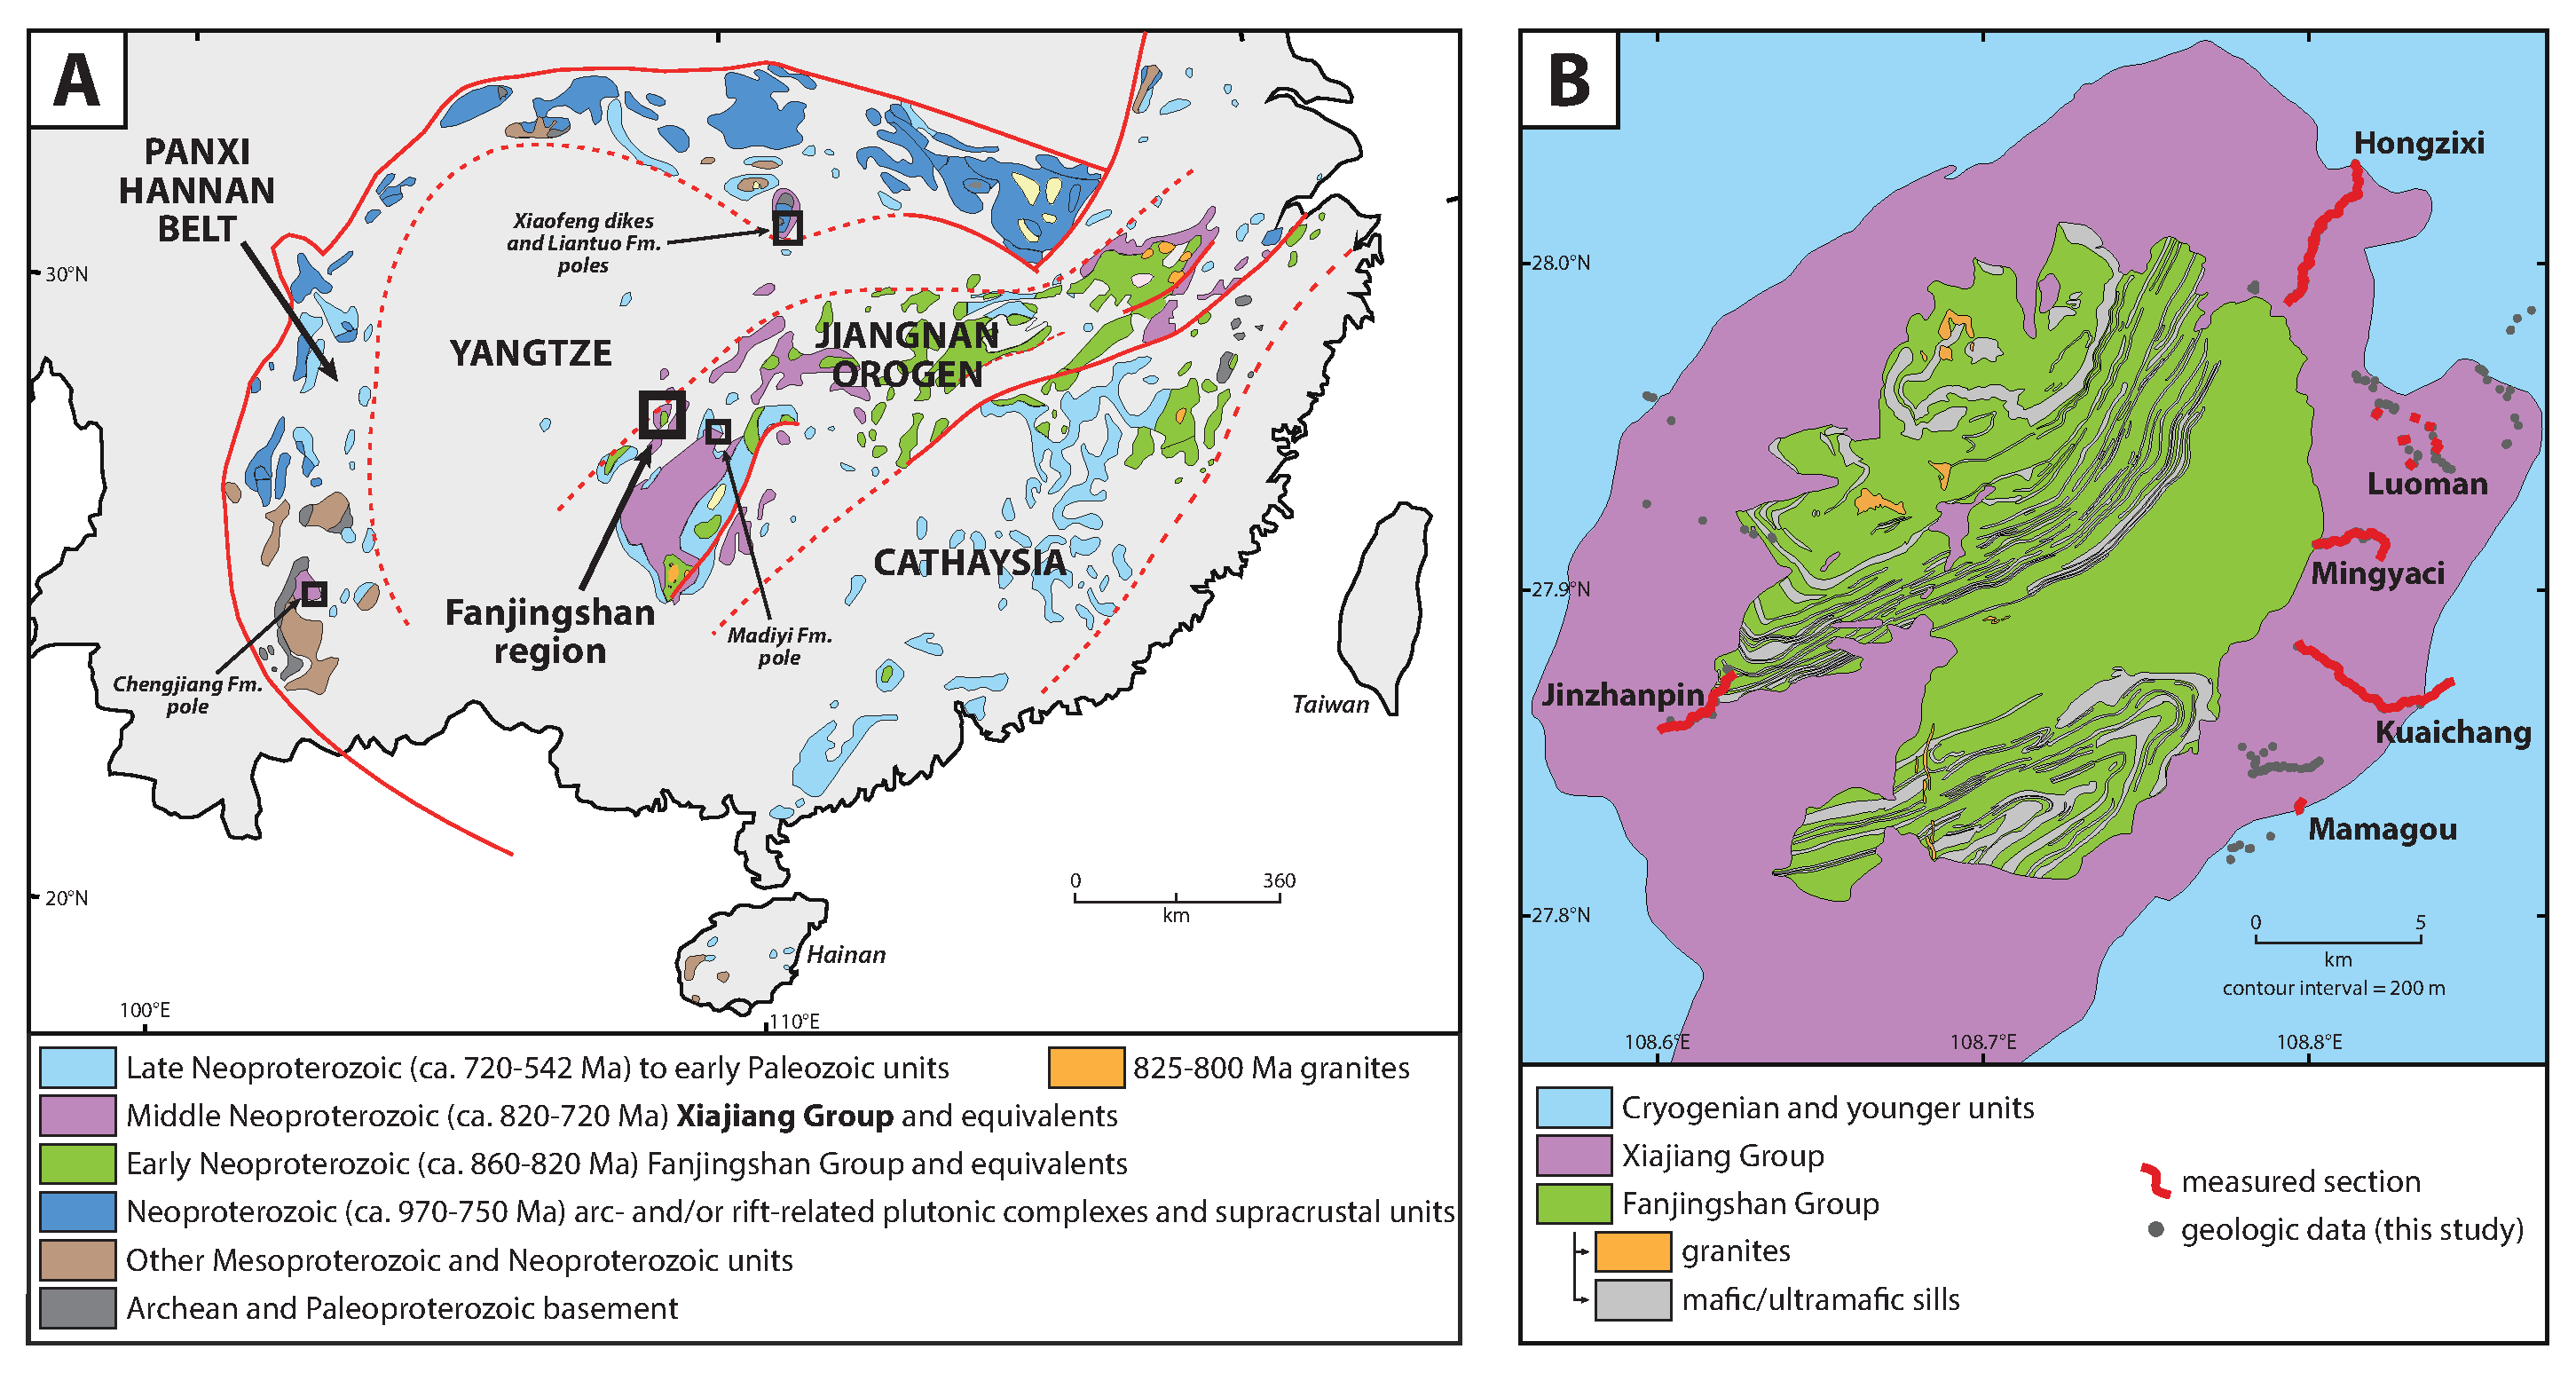
\includegraphics[width=1\textwidth]{figures/Xiajiang/geologic-maps.pdf}
    \caption[Geologic maps of South China and the Fanjingshan region.]{\textbf{A)} Summary geologic map of South China, adapted from \citet{Cawood2017a}, showing the Fanjingshan region from where the Xiajiang Group pole is developed in this study, as well as the localities where other Neoproterozoic poles are developed (Table \ref{tab:South-China-poles}). \textbf{B)} Geologic map of the Fanjingshan region. The distribution of volcanic units within the Fanjingshan Group and the contact between the Fanjingshan and Xiajiang groups were adapted from \citet{Wang2016c}. Both the sedimentary and volcanic units of the Fanjingshan Group were folded, uplifted, and eroded prior to Xiajiang Group deposition. The contact between the Xiajiang Group and the overlying Cryogenian units was adapted from \citet{Zhao2011a}. Unit boundaries were adjusted to be consistent with our geologic data where available. Red lines show the location of the measured stratigraphic sections in Figure \ref{fig:stratigraphic-sections}. Note that the Luoman section consists of seven individually measured sections that were correlated to each other based on local bedding and elevation measurements.}
    \label{fig:geologic-maps}
\end{figure}

\begin{figure}[h!]
    \centering
    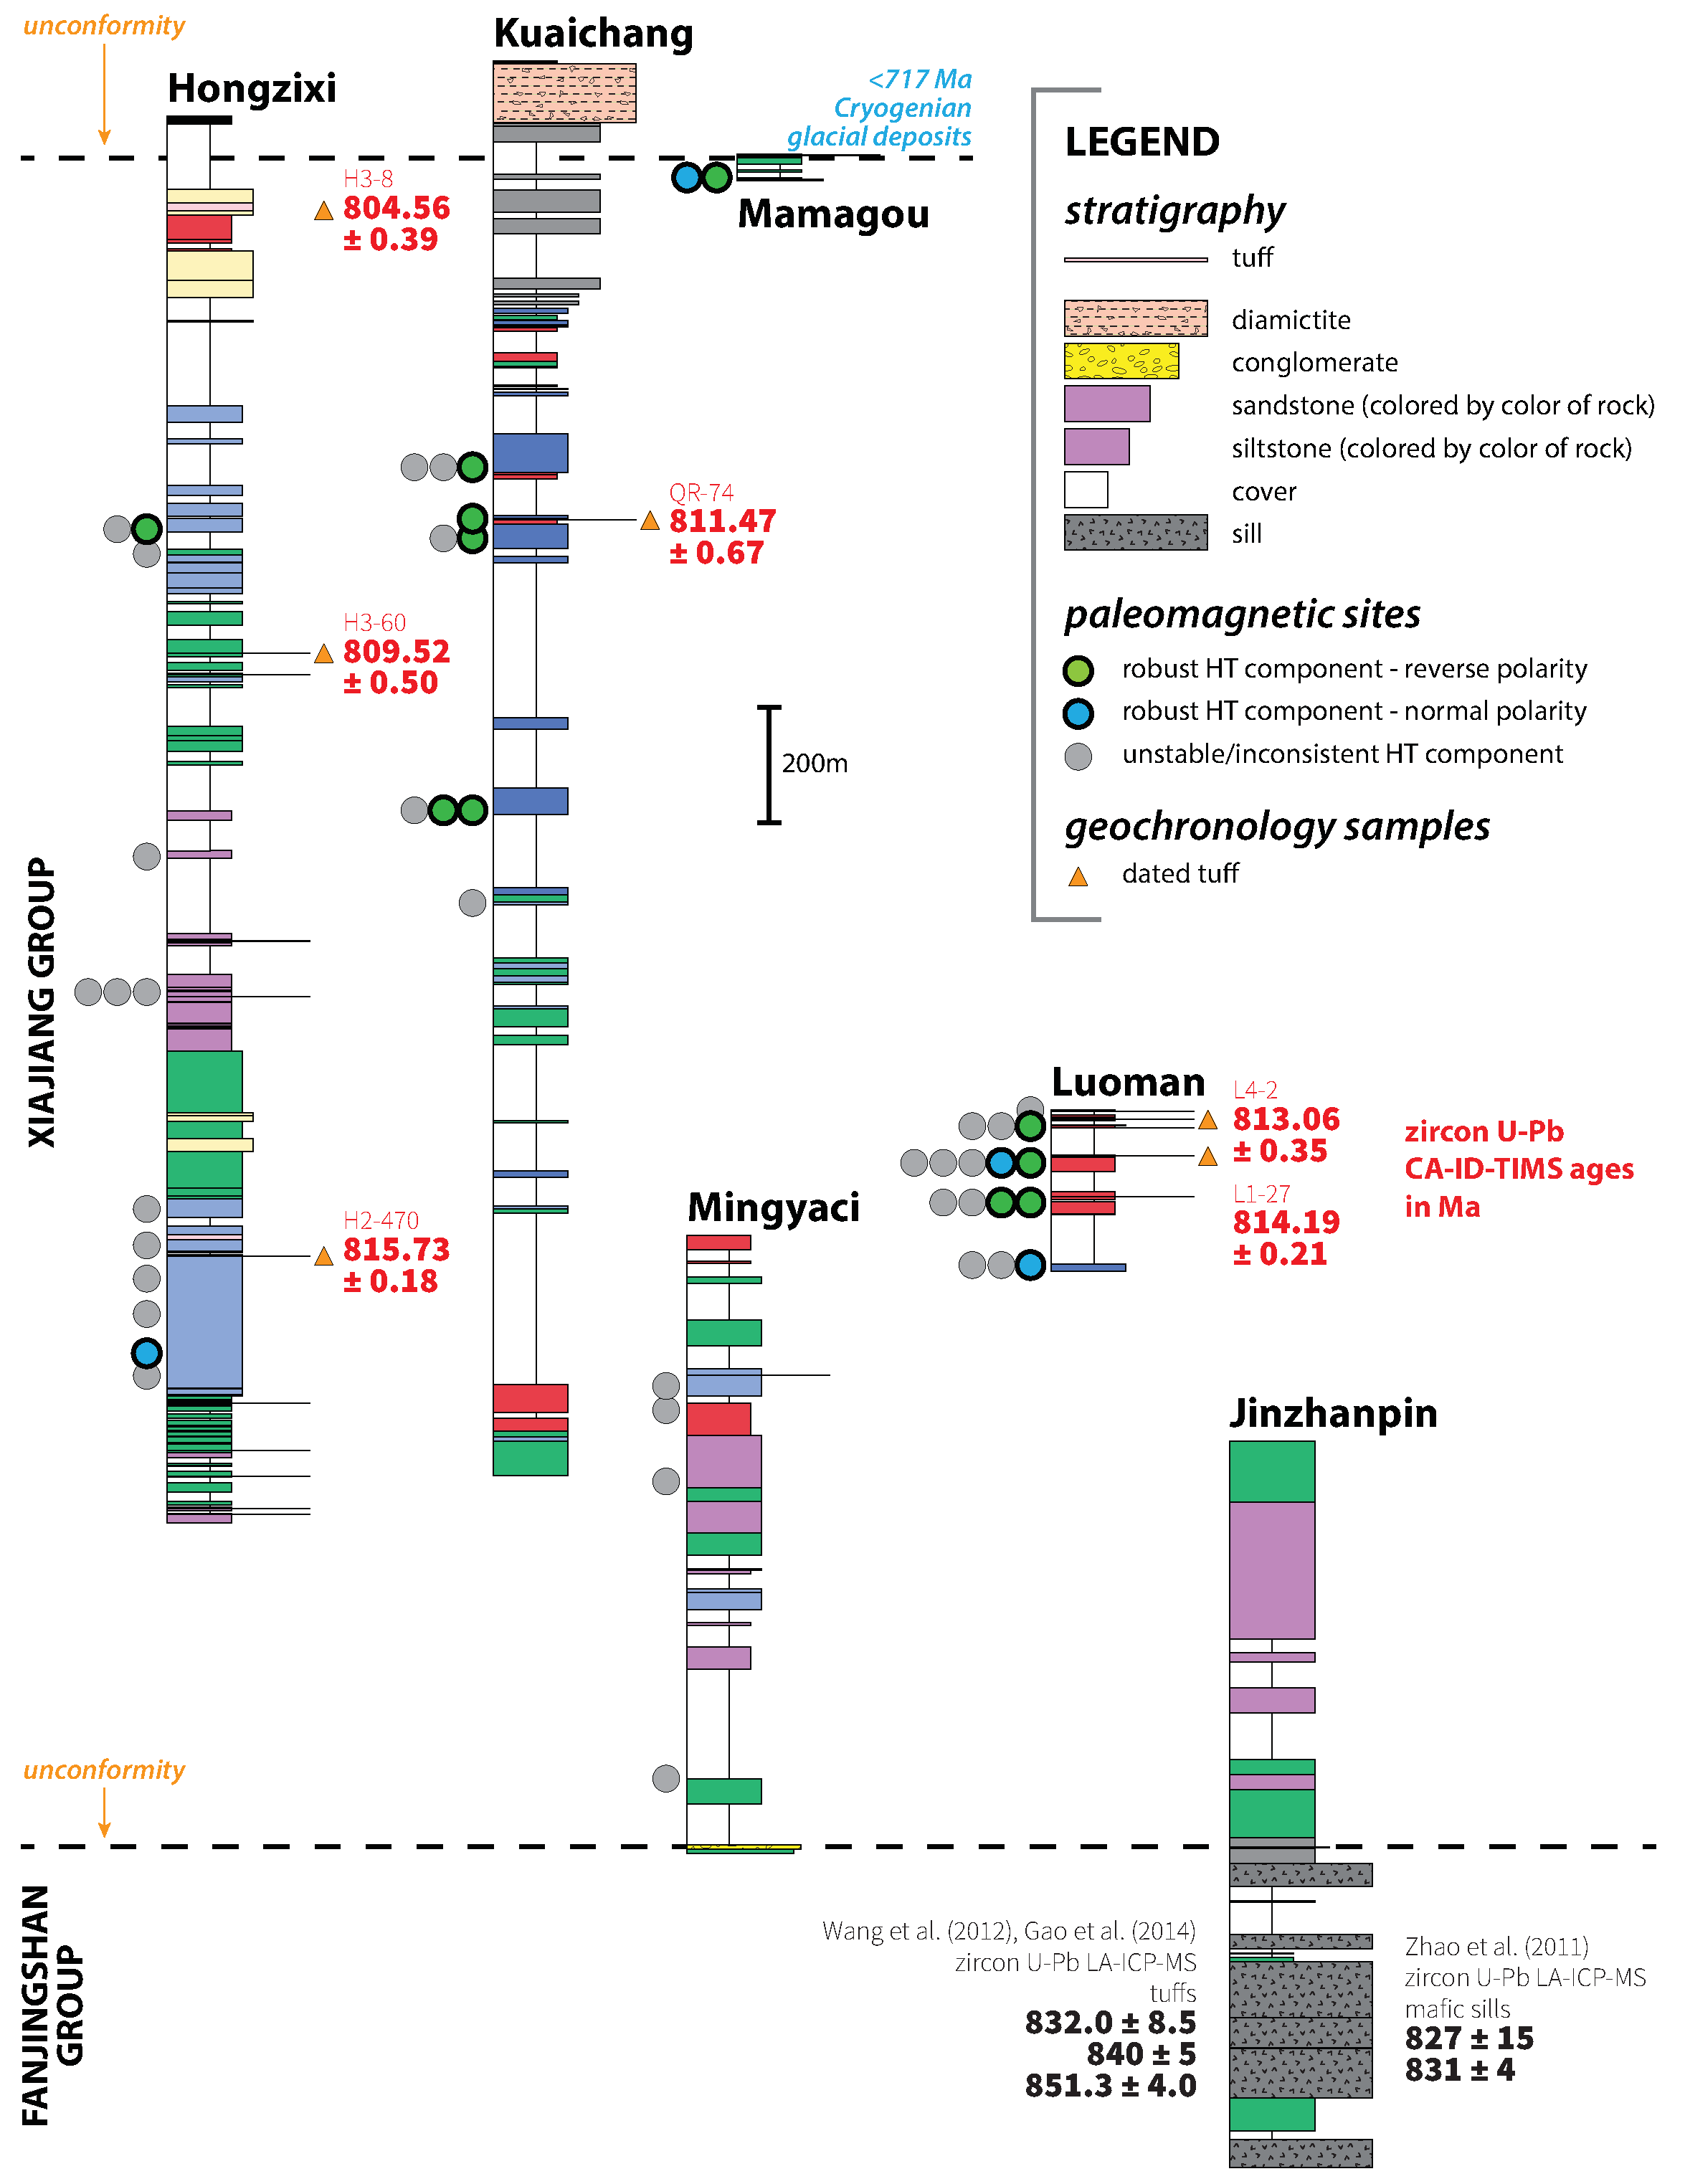
\includegraphics[width=0.80\textwidth]{figures/Xiajiang/stratigraphic-sections.pdf}
    \caption[Stratigraphic sections measured in the Fanjingshan region.]{Stratigraphic sections measured in the Fanjingshan region. Locations of measured sections are shown in Figure \ref{fig:geologic-maps}. The colors are associated with the color of the sedimentary rocks. U-Pb CA-ID-TIMS dates from the Xiajiang Group are from this study and are shown at the stratigraphic levels where the tuffs were collected. The dates from the Fanjingshan Group are not from the section shown, but are from other studies of the rocks elsewhere in the region.}
    \label{fig:stratigraphic-sections}
\end{figure}

Many Proterozoic continental blocks are hypothesized to have come together to form the supercontinent Rodinia during the latest Mesoproterozoic to Neoproterozoic \citep{Hoffman1991a, Li2008a}. However, geochronologic, geologic, and paleomagnetic research continues to refine the configuration of these blocks as well as the timing of their assembly and breakup. At the center of debates regarding the configuration of Rodinia is the South China craton (Fig. \ref{fig:geologic-maps}). For many years, the most widely-used paleogeographic models for the Neoproterozoic adopted the Missing Link model \citep{Li1995a, Li2008a}, which places South China at the core of Rodinia between Australia-East Antarctica and Laurentia. This hypothesis was originally based on the interpretation that the Jiangnan Orogen between the Yangtze and Cathaysia blocks that comprise the South China craton was of similar age to the Grenvillian Orogen of Laurentia (ca. 1.1-1.0~Ga; \citealp{Li1995a}). In this model, the Yangtze block (along with Australia) collides with the Cathaysia block and Laurentia ca. 1.0~Ga \citep{Li1995a}.

Recent geologic, geochemical, and geochronological data have instead interpreted the Jiangnan Orogen to record ongoing accretionary orogenesis of magmatic arc and back arc assemblages along the southeast margin of the Yangtze block in the Tonian up until \textless830~Ma terminal collision with Cathaysia \citep{Cawood2017a, Yan2019a}. In addition to this record of later Tonian magmatism and orogenesis between the Yangtze and Cathaysia blocks, there was accretionary orogenesis and continental arc volcanism along the Panxi-Hannan Belt of the northwest Yangtze block \citep{Cawood2017a}. This record includes both the obduction of ca. 800~Ma ophiolites \citep{Zhao2017a} and ca. 870-706~Ma arc-related magmatism \citep{Dong2012a}. These data indicate that South China was surrounded by active margins with subduction zones through much of the Tonian. This record is difficult to reconcile with a position in the interior of a stable supercontinent. Instead, these data suggest that South China was on the periphery of Rodinia \citep{Cawood2017a}, or disconnected from it entirely \citep{Merdith2017a}. Nevertheless, the Missing Link position for South China, as implemented in \citet{Li2008a}, remains the default in many depictions of Neoproterozoic paleogeography motivating the need for further development of paleogeographic constraints.

\section{Geologic Setting}

This study presents paleomagnetic and U-Pb chemical abrasion isotope dilution thermal ionization mass spectrometry (CA-ID-TIMS) zircon geochronologic data from the Xiajiang Group in the Fanjingshan region of Guizhou province, China (Fig. \ref{fig:geologic-maps}A). The Fanjingshan region lies within the Jiangnan orogenic belt that separates the Yangtze and Cathaysia blocks of the South China craton, and is characterized by a regional anticline that developed in the Mesozoic (Fig. \ref{fig:geologic-maps}B; \citealp{Li2016c, Ma2019a}). At the core of the anticline is the Fanjingshan Group, dominantly composed of sandstones intruded by intermediate to ultramafic sills (Fig. \ref{fig:geologic-maps}B; \citealp{Wang2014a}). These sills are interpreted to have formed in a subduction-related environment just prior to amalgamation of the Yangtze and Cathaysia blocks \citep{Wang2014a}.

Both the sedimentary rocks and the intrusive sills of the Fanjingshan Group are folded, and are separated from the overlying Xiajiang Group by an angular unconformity (Fig. \ref{fig:geologic-maps}B). Tuffs of the Fanjingshan Group in the Fanjingshan region have yielded U-Pb laser ablation inductively coupled plasma mass spectrometry (LA-ICP-MS) zircon dates of 851.3$\pm$4.0~Ma, 840$\pm$5~Ma, and 832.0$\pm$8.5~Ma \citep{Wang2012d, Gao2014a}. U-Pb LA-ICP-MS zircon dates for the mafic sills are 831$\pm$4~Ma and 827$\pm$15~Ma \citep{Zhao2011a}, and U-Pb LA-ICP-MS detrital zircon dates within the sediments are as young as 849$\pm$6.5~Ma \citep{Zhao2011a}. These dates constrain the exposure, folding, and erosion of the Fanjingshan Group to have been after ca. 830~Ma. A cobble to boulder conglomerate is often the lowest unit of the Xiajiang Group, before the stratigraphy transitions into hundreds of meters of red, purple, green, and grey-blue graded beds of siltstone and fine-grained sandstone interbedded with volcanic ashes (Fig. \ref{fig:stratigraphic-sections}). The fine-grained sandstone-siltstone interbeds locally exhibit ripple cross-stratification, which are interpreted to have formed as Bouma-C beds associated with distal turbidity currents. The presence of $\sim$1--5~cm volcanic ashes throughout the stratigraphy without lithic fragments indicate the presence of a nearby, but not immediately adjacent, volcanic arc. Existing U-Pb LA-ICP-MS zircon dates for tuffs of the Xiajiang Group in the Fanjingshan region of 814.0$\pm$6.3~Ma and 813.5$\pm$9.6~Ma \citep{Gao2010a, Gao2014a} suggest deposition of Xiajiang Group began by ca. 815~Ma. Unconformably overlying the Xiajiang Group in the Fanjingshan region are glacial deposits correlated with the Cryogenian Sturtian `Snowball Earth' glaciation (referred to locally as the Tiesi'ao Formation; \citealp{Xiong2014a}). Geochronologic constraints from South China, Laurentia, Oman, and the Arabian-Nubian Shield indicate that onset of the Sturtian glaciation was rapid and globally synchronous within the available precision of the geochronology \citep{Bowring2007a, Macdonald2010a, MacLennan2018a, Lan2020a}. These constraints on the Sturtian glaciation constrain Xiajiang Group deposition to have ended prior to ca. 717~Ma. No continuous individual section was identified that captures both the Fanjingshan-Xiajiang Group contact and the contact between the Xiajiang Group and the Sturtian glacial deposits (Fig. \ref{fig:stratigraphic-sections}). However, correlation of individually measured sections based on aligning the bounding unconformities of the Xiajiang Group and the geochronologic results suggests that the Xiajiang Group is $\sim$3000~m thick in this region (Fig. \ref{fig:stratigraphic-sections}).

We note that the nomenclature of pre-Sturtian Neoproterozoic strata in South China varies in the literature. In some publications, the term the `Banxi Group' is used to refer to any ca. 815--717~Ma sediments in South China, including those in our study area (e.g. \citealp{Zhao2011a, Zhang2019c}). In other publications, the term the `Banxi Group' is used to refer exclusively to ca. 815--717~Ma sediments in the Hunan province, and equivalent strata in our study area in the Guizhou province is referred to as the `Xiajiang Group' (e.g. \citealp{BGMRGZ1984a, Wang2014a, Xiong2014a, Geng2015a, Li2016b, Wang2016c, Yan2019a}). Further to the southeast, sedimentary rocks interpreted to correlate with the Banxi and Xiajiang Groups are referred to as the `Danzhou Group' \citep{Yan2019a}. There are similar regional nomenclature differences for the older Fanjingshan Group, which is referred to as the `Fanjingshan Group' in our study area and is correlated with units known as the `Lengjiaxi Group' and the `Sibao Group' elsewhere, and the younger Tiesi'ao Formation, which is referred to as the `Tiesi'ao Formation' in our study area and is correlated with units known as the `Chang'an Formation' elsewhere. In this study, we follow the nomenclature most widely used for the Guizhou province, using the term Fanjingshan Group, and referring to the sediments unconformably bounded by the Fanjingshan Group and Sturtian glacial deposits in the Fanjingshan region as the Xiajiang Group.

\section{Methods}

\subsection{Paleomagnetism}

Where exposure of the stratigraphy was good, sections were measured using a Jacob’s staff. In cases where vegetation obscured the stratigraphy for hundreds of meters, the thickness of covered stratigraphy was estimated based on GPS measurements and local bedding orientations, leading to the covered intervals shown in Figure \ref{fig:stratigraphic-sections}.

Cores from the studied sedimentary rocks were collected using a gas-powered drill and a Pomeroy orienting device. Sun compass data were used for sample orientations when possible, and magnetic compass orientations were used when necessitated by cloud cover. Sample collection was organized into `sites,' where each site consists of a set of samples that were obtained from within a few meters of stratigraphy. This grouping provides a useful organizational framework although it does not correspond to the definition of a site within the framework of the MagIC database wherein every sample in a site should be expected to record a direction from the same moment in time. In most cases, cores were collected from the least foliated purple/red siltstone of the Xiajiang Group, but when no such lithologies were present, green/grey-blue siltstones were also collected.

Thermal demagnetization and magnetic remanence measurements were conducted at UC Berkeley and the China University of Geosciences, Beijing. At the UC Berkeley Paleomagnetism Laboratory, measurements were made using a 2G Enterprises DC-SQUID superconducting rock magnetometer equipped with an automated pick-and-place sample changer system \citep{Kirschvink2008a}. The magnetometer is housed in a magnetostatic shield with magnetic fields \textless500~nT. A quartz glass sample rod brings the samples into the measurement region and is typically measured at $\sim5\times10^{-12}$~Am$^{2}$. After measurement of the natural remanent magnetization (NRM), the samples were progressively step-heated and thermally demagnetized in an ASC thermal specimen demagnetizer (residual fields \textless10~nT).

At the China University of Geosciences, Beijing, paleomagnetic analyses were conducted in a magnetically shielded room with a residual field of \textless300~nT in the Laboratory of Paleomagnetism and Environmental Magnetism. Magnetic remanence was measured using a 2G 755-4~K three-axis cryogenic magnetometer, and stepwise thermal demagnetizations were carried out with an ASC TD-48 or MMTDSC furnace, both of which have an internal residual field of \textless10~nT.

All paleomagnetic data to the measurements level, as well as interpreted fits made using the PmagPy software package \citep{Tauxe2016a}, are available in the MagIC database (https://earthref.org/MagIC/doi/).

\subsection{Geochronology}

Tuffs collected for U-Pb geochronology typically appear as $\sim$1--5~cm horizons within the Xiajiang Group of the Fanjingshan region. Their tan/white color is distinguishable from the purple/red/green/grey-blue of the adjacent siltstone and fine sandstone. In some cases, the exposed surface of the tuffs have weathered into a clay-rich unlithified mud, likely due to the weathering of the volcanic ash to clays (e.g. bentonite). In these cases, the mud was removed before sampling of the lithified tuff. All samples were scrubbed with steel brushes to remove any recent detritus prior to further analysis.

Zircon grains were isolated from the bulk rock by standard mineral separation techniques. All zircon grains analyzed in this study employed the protocols and data reduction outlined in \citet{Meyers2012a}. Prior to dissolution, zircon grains were subjected to a modified chemical abrasion in order to remove radiation-damaged zones of the zircon and minimize the effects of Pb loss \citep{Mattinson2005a}. The accuracy of the $^{238}$U/$^{206}$Pb dates presented herein is controlled by the gravimetric calibration of the EARTHTIME U-Pb tracer employed in this study and the determination of the $^{238}$U decay constant \citep{Jaffey1971a, Condon2015a}. Unless stated otherwise, uncertainties on U-Pb dates reported in this manuscript are the internal (analytical) uncertainties in the absence of external or systematic errors, with these additional uncertainties reported in Table \ref{tab:SChina-geochronology}.

\section{Results}

\subsection{Paleomagnetism}

\begin{table}[h!]
\caption[Paleomagnetic results for the Xiajiang Group of the Fanjingshan region.]{Paleomagnetic results for individual sites with stable and consistent high temperature components in the Xiajiang Group of the Fanjingshan region.}
\vspace{0.25cm}
\resizebox{\linewidth}{!}{
	\begin{tabular}{lllccccccccc}
	\hline
	\textbf{site} & \textbf{section} & \textbf{lab} & \textbf{site lat.} & \textbf{site lon.} & \textbf{n} & \textbf{dec$_{1.0}$} & \textbf{inc$_{1.0}$} & \textbf{dec$_{0.6}$} & \textbf{inc$_{0.6}$} & \textbf{$\alpha_{95}$} & \textbf{polarity} \\
	&&&&&&&&&&& \\
    TR007 & Hongzixi & Beijing & 27.991 & 108.797 & 13 & 14.1 & 64.4 & 14.1 & 73.9 & 8.9 & N \\
    TR014 & Hongzixi & Berkeley & 28.014 & 108.805 & 12 & 150.2 & -66.8 & 330.2 & 75.6 & 12.1 & R \\
    TR018 & Kuaichang & Berkeley & 27.867 & 108.820 & 14 & 208.3 & -64.0 & 28.3 & 73.7 & 14.2 & R \\
    TR020 & Kuaichang & Berkeley & 27.866 & 108.821 & 10 & 111.6 & -76.9 & 291.6 & 82.1 & 11.2 & R \\
    TR021 & Kuaichang & Beijing & 27.864 & 108.822 & 9 & 208.0 & -71.5 & 28.0 & 78.6 & 17.0 & R \\
    TR024 & Kuaichang & Berkeley & 27.872 & 108.811 & 9 & 124.9 & -63.5 & 304.9 & 73.3 & 18.2 & R \\
    TR026 & Kuaichang & Berkeley & 27.872 & 108.811 & 9 & 150.3 & -85.7 & 330.3 & 87.4 & 16.0 & R \\
    TR004a & Mamagou & Berkeley & 27.835 & 108.797 & 10 & 334.8 & 71.4 & 334.8 & 78.6 & 8.2 & N \\
    TR004b & Mamagou & Berkeley & 27.835 & 108.797 & 5 & 106.4 & -75.9 & 286.4 & 81.4 & 12.6 & R \\
    TR031 & Luoman & Beijing & 27.938 & 108.831 & 8 & 337.6 & 65.2 & 337.6 & 74.5 & 14.5 & N \\
    TR034 & Luoman & Beijing & 27.939 & 108.831 & 11 & 291.6 & -75.9 & 111.6 & 81.5 & 13.0 & R \\
    TR035 & Luoman & Berkeley & 27.954 & 108.821 & 19 & 42.4 & 68.4 & 42.4 & 76.6 & 14.9 & N \\
    TR037 & Luoman & Beijing & 27.946 & 108.829 & 17 & 202.1 & -86.3 & 22.1 & 87.8 & 17.2 & R \\
    TR039 & Luoman & Beijing & 27.946 & 108.829 & 9 & 136.8 & -78.1 & 316.8 & 82.8 & 21.2 & R \\
    TR042 & Luoman & Berkeley & 27.943 & 108.839 & 14 & 131.5 & -71.9 & 311.5 & 78.9 & 11.5 & R \\
	\hline
	\end{tabular}}

\scriptsize
\flushleft \emph{Notes:} \\
(1) All directions are for the high temperature component.\\
(2) \textbf{dec$_{1.0}$} and \textbf{inc$_{1.0}$} refer to the declination and inclination of the mean tilt-corrected direction, without correcting for polarity or inclination shallowing.\\
(3) \textbf{dec$_{0.6}$} and \textbf{inc$_{0.6}$} refer to the declination and inclination of the mean tilt-corrected direction, after correcting for polarity and inclination shallowing using a flattening factor of 0.6.\\
(4) For the \textbf{polarity}, we interpret the mean directions with a positive inclination as normal polarity (N), and the mean directions with a negative inclination as reverse polarity (R).
\label{tab:site-means}
\end{table}

\begin{figure}[h!]
    \centering
    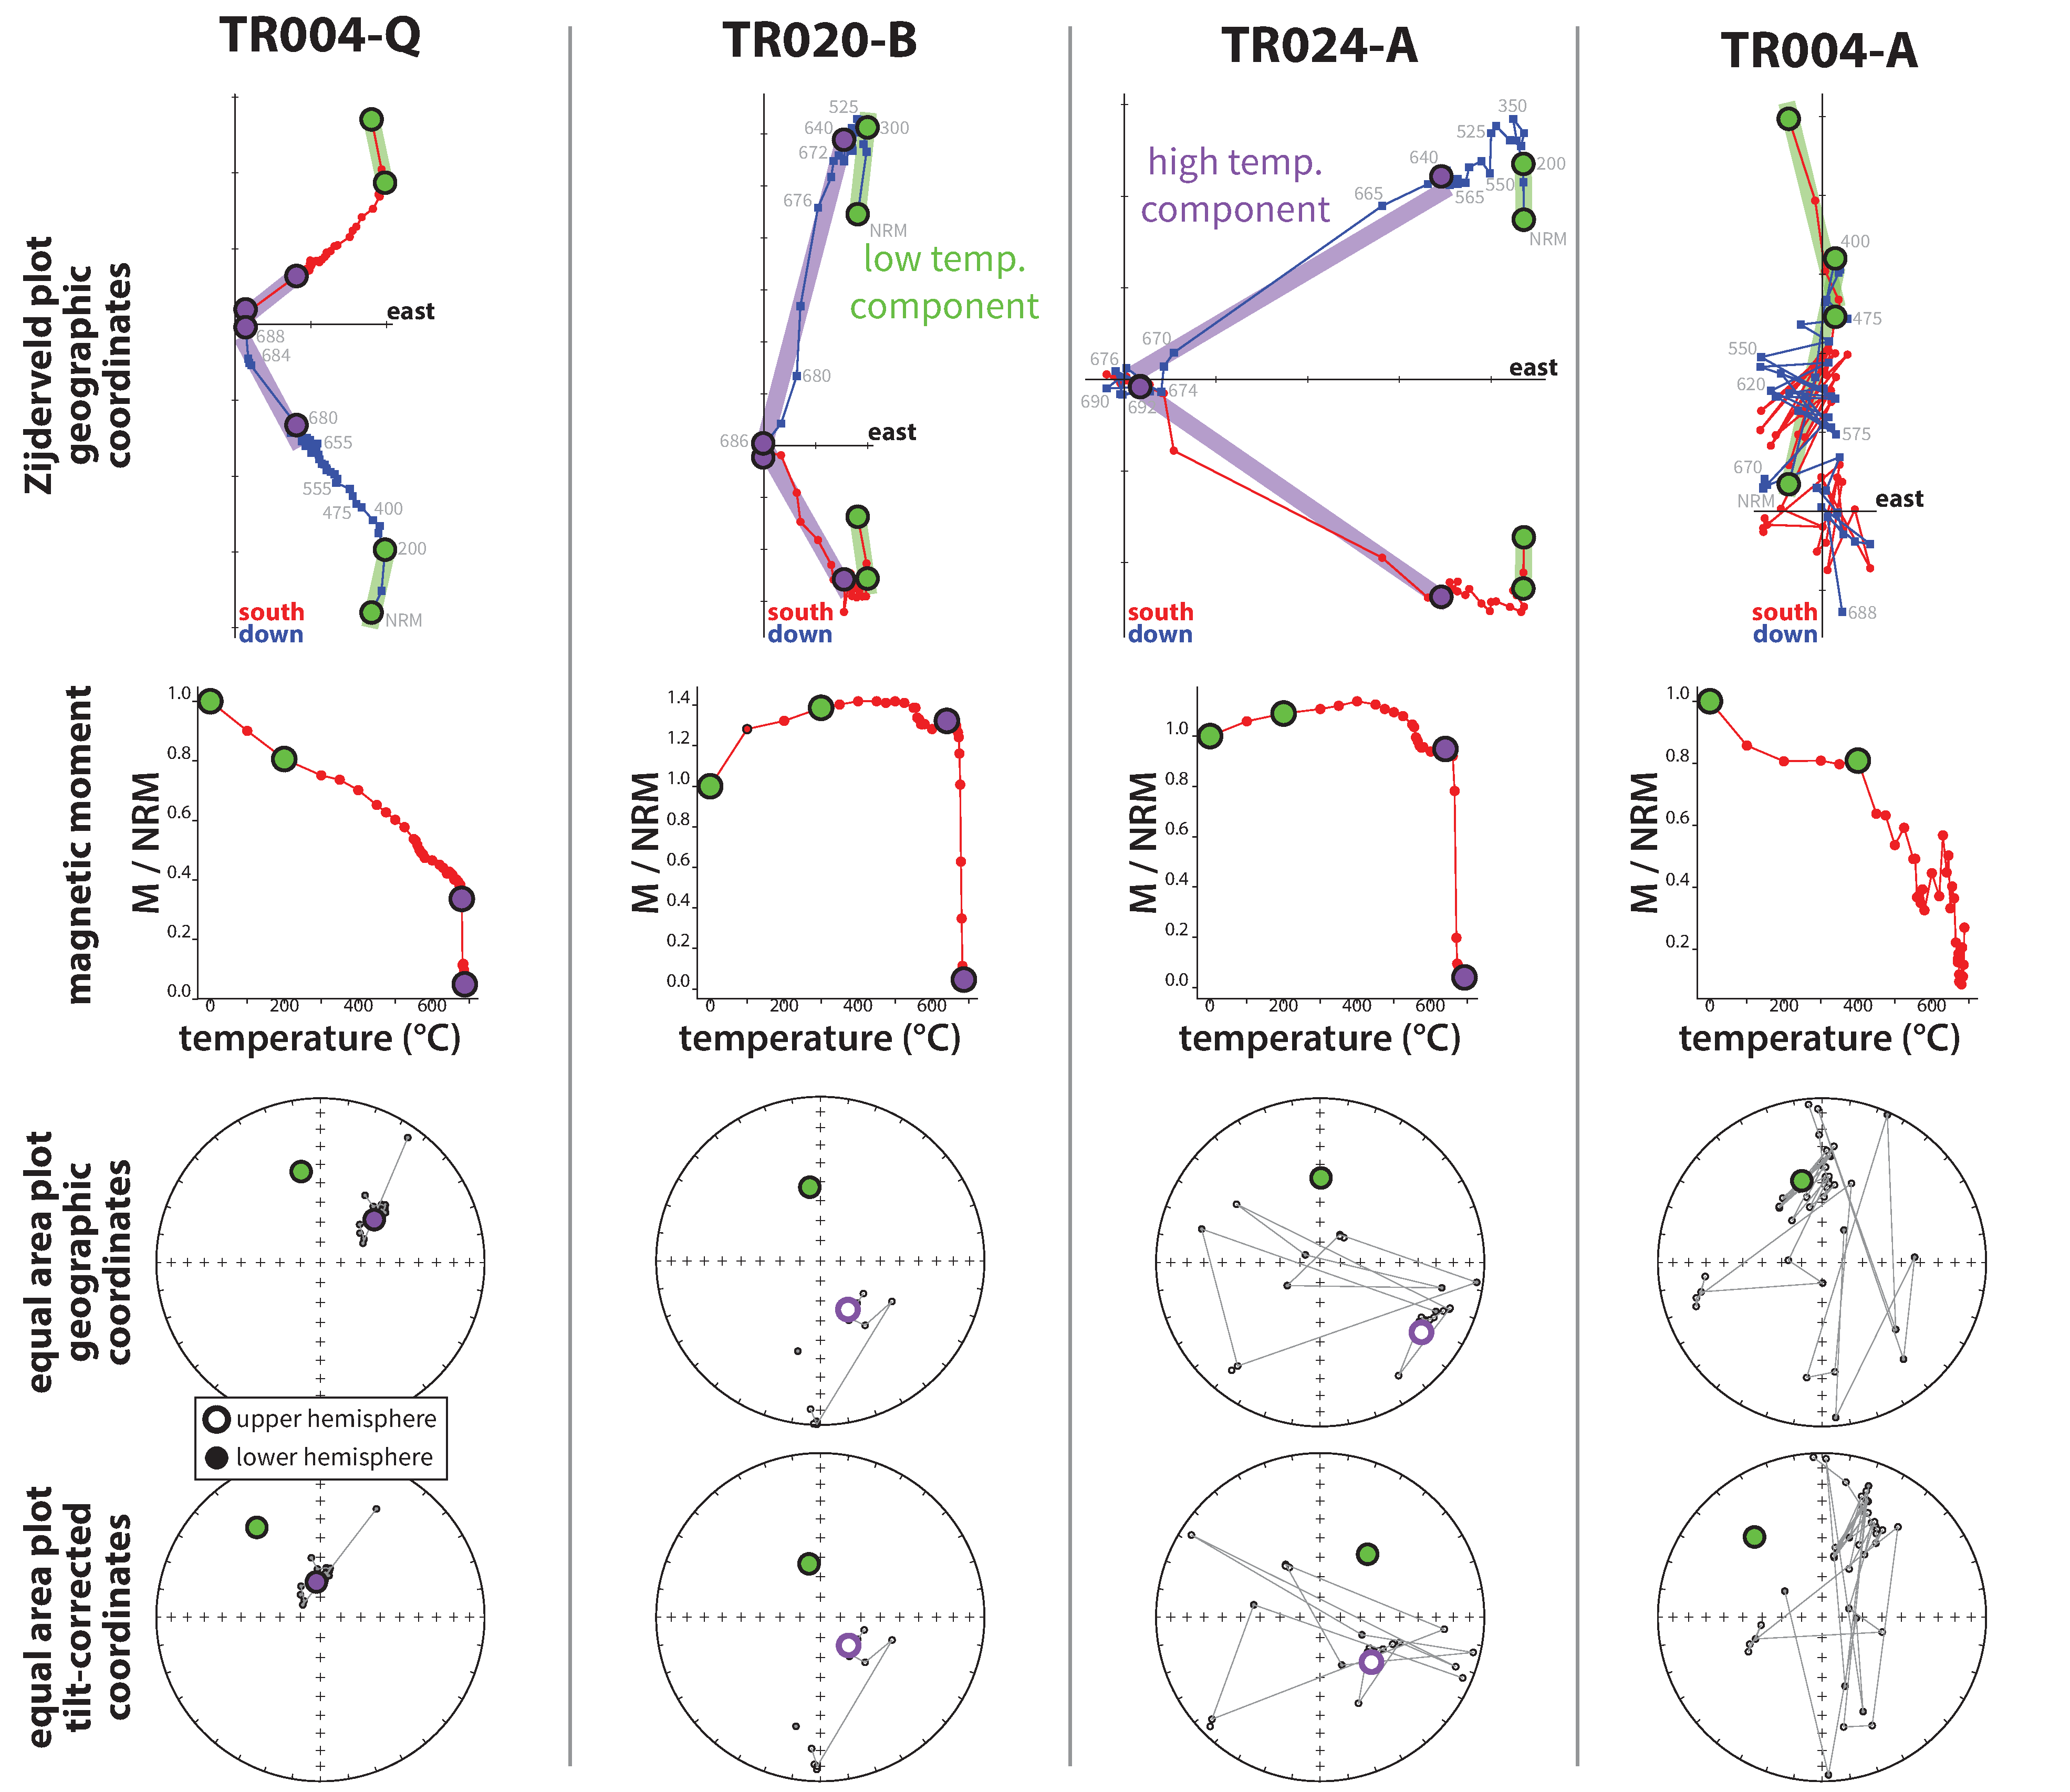
\includegraphics[width=\textwidth]{figures/Xiajiang/representative-specimens.pdf}
    \caption[Thermal demagnetization results.]{Thermal demagnetization results. Specimens TR004-Q, TR020-B, and TR024-A exhibit magnetic behaviour typical of specimens that yield a stable and consistent high temperature component. Specimen TR004-Q exhibits magnetic behaviour typical of specimens that do not yield a stable high temperature component. In the Zijderveld plots, the specimen magnetizations at a given thermal demagnetization step (grey numbers) are shown (NRM = natural remanent magnetization). Fits to the low and high temperature components are shown in green and purple respectively. Note that the Zijderveld plots and the upper equal area plots are in geographic coordinates, whereas the lower equal area plot is in tilt-corrected coordinates.}
    \label{fig:representative-specimens}
\end{figure}

\begin{figure}[h!]
    \centering
    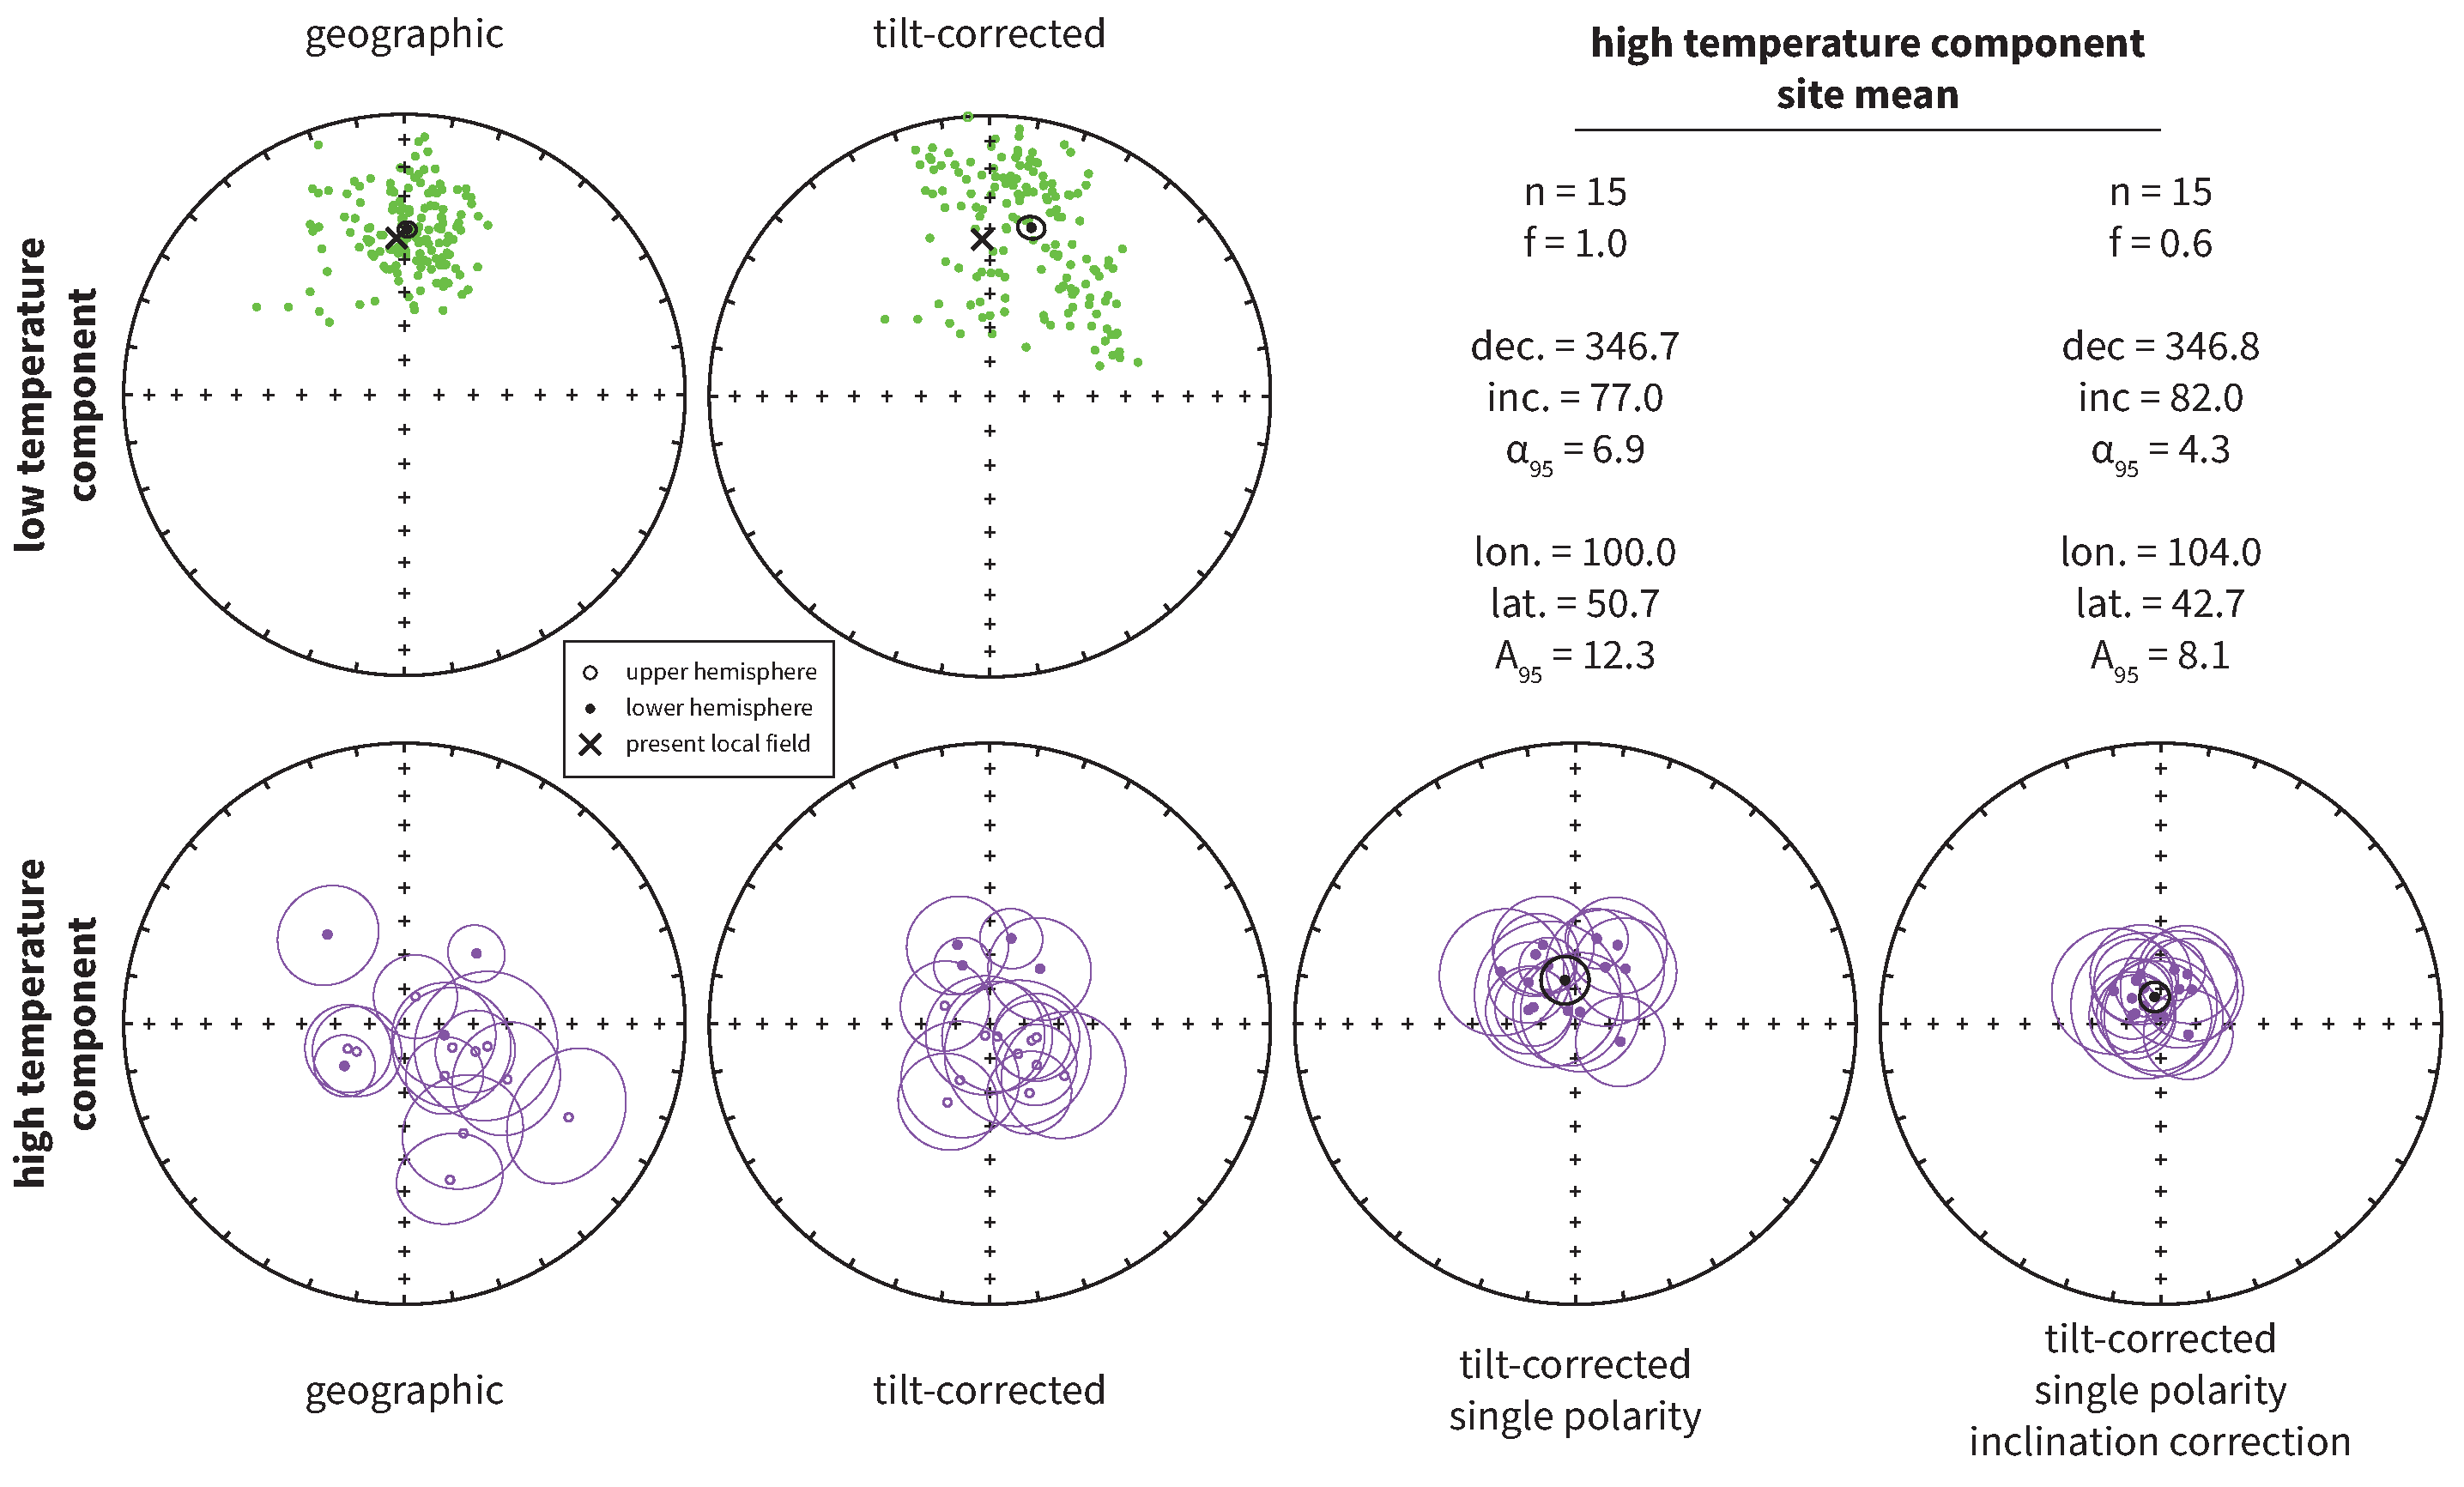
\includegraphics[width=\textwidth]{figures/Xiajiang/site-means.pdf}
    \caption[Paleomagnetic results for the Xiajiang Group of the Fanjingshan region.]{Paleomagnetic results for sites that yielded specimens with stable and consistent high temperature components in the Xiajiang Group of the Fanjingshan region (Table \ref{tab:site-means}). For the low temperature component, each point represents an individual specimen. For the high temperature component, each point and associated uncertainty ellipse represents the specimen mean for individual sites. The reported site means are the means of these specimen means.}
    \label{fig:site-means}
\end{figure}

Thermal demagnetization data from siltstones of the Xiajiang Group in the Fanjingshan region show variable behaviour from site to site. A component removed during initial thermal demagnetization steps (\textless300\degreesC) is present in most samples and typically yields a direction that is consistent with a present local field overprint acquired via viscous remanent magnetization (Fig. \ref{fig:representative-specimens}). Samples within 29 of the 44 sites yield either unstable or inconsistent behaviour at temperatures \textgreater300\degreesC. However, the remaining 15 sites yield stable and consistent behaviour at high temperatures. This high-temperature component is well-fit by least-squares lines that intersect the origin on a Zijderveld plot between $\sim$650 and $\sim$690\degreesC (Fig. \ref{fig:representative-specimens}). These high unblocking temperatures are close to the N\'eel temperature of \textgreater500~nm hematite, and are therefore consistent with the high-temperature component being dominantly held by primary detrital hematite rather than finer-grained authigenic pigmentary hematite \citep{Dunlop2001a, Jiang2015a, Swanson-Hysell2019b}.

Two polarities are recorded by the high-temperature component. Of the 15 successful sites, 4 sites yield normal polarity (positive inclination) directions, while the other 11 sites yield reversed polarity (negative inclination) directions (Figs. \ref{fig:stratigraphic-sections} and \ref{fig:site-means}; Table \ref{tab:site-means}). We interpret positive inclinations to correspond to normal geomagnetic polarity, although we recognize that a correlation of positive inclination to reversed geomagnetic polarity could be permissible in alternative paleogeographic reconstructions. When all sites are converted into a single polarity, the null hypothesis that the specimen mean directions of the normal and reversed polarity sites were drawn from distributions that share a common mean direction can not be rejected at the 95\% confidence level (in the Watson V test, $V$ = 4.9 and $V_{crit}$ = 7.4). Since $V<V_{crit}$, the two polarities recorded by the high-temperature component pass a reversal test after tilt corrections are applied to the high-temperature component site mean directions.

A bootstrap fold test \citep{Tauxe1994a} finds that the tightest grouping of site mean directions is obtained between 68 and 103\% unfolding at the 95\% confidence level (Fig. S1). Since this range of unfolding encompasses 100\%, the high temperature component passes a fold test, thereby constraining the high-temperature component to have been acquired prior to Mesozoic folding of the Xiajiang Group \citep{Li2016c, Ma2019a}.

Based on the high unblocking temperatures characteristic of detrital hematite, the positive reversal test, and the positive fold test, we interpret the high temperature component (Fig. \ref{fig:site-means}) as being primary and acquired at the time of deposition.

Deposition and burial compaction can result in detrital hematite magnetization being shallower in inclination than the local magnetic field direction at the time of deposition \citep{Tauxe2005a, Bilardello2016a}. The degree to which the inclination ($I$) has been shallowed can be expressed by the flattening factor ($f$) in the equation $\tan(I_{observed}) = f\tan(I_{original})$, where $f=1$ indicates no inclination shallowing and $f=0$ indicates a completely flattened direction \citep{King1955a}. Although the flattening factor in any given sedimentary unit depends on a variety of factors such as the composition of the sediment, values of $f$ obtained from empirical studies of detrital hematite-bearing rocks can be reasonably well-explained by a normal distribution about a mean of $\sim$0.6 \citep{Tauxe1984a, Bilardello2016a}. We therefore apply this empirically-derived inclination correction ($f=0.6$) to the specimen means obtained from individual sites (Fig. \ref{fig:site-means}), and interpret the resulting direction as approximating the direction of the geomagnetic field at the time of deposition. Directions and poles calculated with and without this inclination correction are shown in Figures \ref{fig:site-means} and \ref{fig:SChina-APWP}.

\subsection{Geochronology}

\begin{table}[h!]
\caption[CA-ID-TIMS $^{206}$Pb/$^{238}$U dates from tuffs developed in this study.]{Summary of CA-ID-TIMS $^{206}$Pb/$^{238}$U dates from tuffs developed in this study.}
\vspace{0.25cm}
\resizebox{\linewidth}{!}{
    \begin{tabular}{lcclcccccccc}
    \hline
    \textbf{sample} & \textbf{latitude} & \textbf{longitude} & \textbf{section} & \textbf{stratigraphic} & \textbf{$^{206}$Pb/$^{238}$U} & \multicolumn{3}{c}{\textbf{error (2$\sigma$)}} & \textbf{MSWD} & \textbf{n} & \textbf{N} \\
    & \textbf{$^{\circ}$N} & \textbf{$^{\circ}$E} & & \textbf{height (m)} & \textbf{date (Ma)} & \textbf{X} & \textbf{Y} & \textbf{Z} & & \\
    &&&&&&&& \\
    \multicolumn{11}{l}{\textit{Xiajiang Group of the Fanjingshan region (Guizhou province)}} \\
    H2-470 & 27.99396 & 108.79792 & Hongzixi & 1586.2 & 815.73 & 0.18 & 0.28 & 0.92 & 1.6 & 6 & 16 \\
    L1-27 & 27.93856 & 108.83107 & Luoman & 1752.3 & 814.19 & 0.21 & 0.31 & 0.92 & 1.7 & 5 & 9 \\
    L4-2 & 27.94335 & 108.83931 & Luoman & 1815.5 & 813.06 & 0.35 & 0.48 & 1.0 & 1.8 & 3 & 4 \\
    H3-60 & 28.01002 & 108.80240 & Hongzixi & 2622.4 & 809.52 & 0.50 & 0.62 & 1.1 & 1.9 & 6 & 10 \\
    QR-74 & 27.86578 & 108.82076 & Kuaichang & 2850.3 & 811.47 & 0.67 & 0.77 & 1.2 & 1.9 & 3 & 6 \\
    H3-8 & 28.02468 & 108.81506 & Hongzixi & 3389.3 & 804.56 & 0.39 & 0.52 & 1.0 & 0.6 & 3 & 4 \\\\
    \multicolumn{11}{l}{\textit{Madiyi Formation in the Zhijiang region (Hunan province})} \\
    ZJ-B & 27.5 & 109.6 & - & - & 804.90 & 0.36 & 0.49 & 0.99 & 0.9 & 5 & 6 \\\\
    \multicolumn{11}{l}{\textit{Liantuo Formation in the Three Gorges region (Hubei province)}} \\
    FDM14-1 & 30.8527 & 111.1512 & - & - & 779.52 & 0.26 & 0.38 & 0.92 & 2.0 & 8 & 16 \\
    \hline
    \end{tabular}}

\scriptsize
\flushleft \emph{Notes:} \\
(1) \textbf{stratigraphic height} is the estimated composite stratigraphic height derived from correlation of individually measured sections based on aligning the bounding unconformities of the Xiajiang Group and the geochronologic results.\\
(2) For the \textbf{errors}, \textbf{X} is the internal (analytical) uncertainty in the absence of external or systematic errors, \textbf{Y} is the uncertainty incorporating the U-Pb tracer calibration error, and \textbf{Z} is the uncertainty including X and Y, as well as $^{238}$U decay constant uncertainty (0.108$\%$; \citealp{Jaffey1971a}). This Z error needs to be utilized when comparing to dates developed using other decay systems (e.g., $^{40}$Ar/$^{39}$Ar, $^{187}$Re-$^{187}$Os).\\
(3) \textbf{MSWD} is the mean square of weighted deviates\\
(4) \textbf{n} is the number of individual zircon dates included in the calculated weighted sample mean date.\\
(5) \textbf{N} is the total number of individual zircons analyzed.\\
(6) Data for individual zircons are provided in the Supporting Information.
\label{tab:SChina-geochronology}
\end{table}

\begin{figure}[h!]
    \centering
    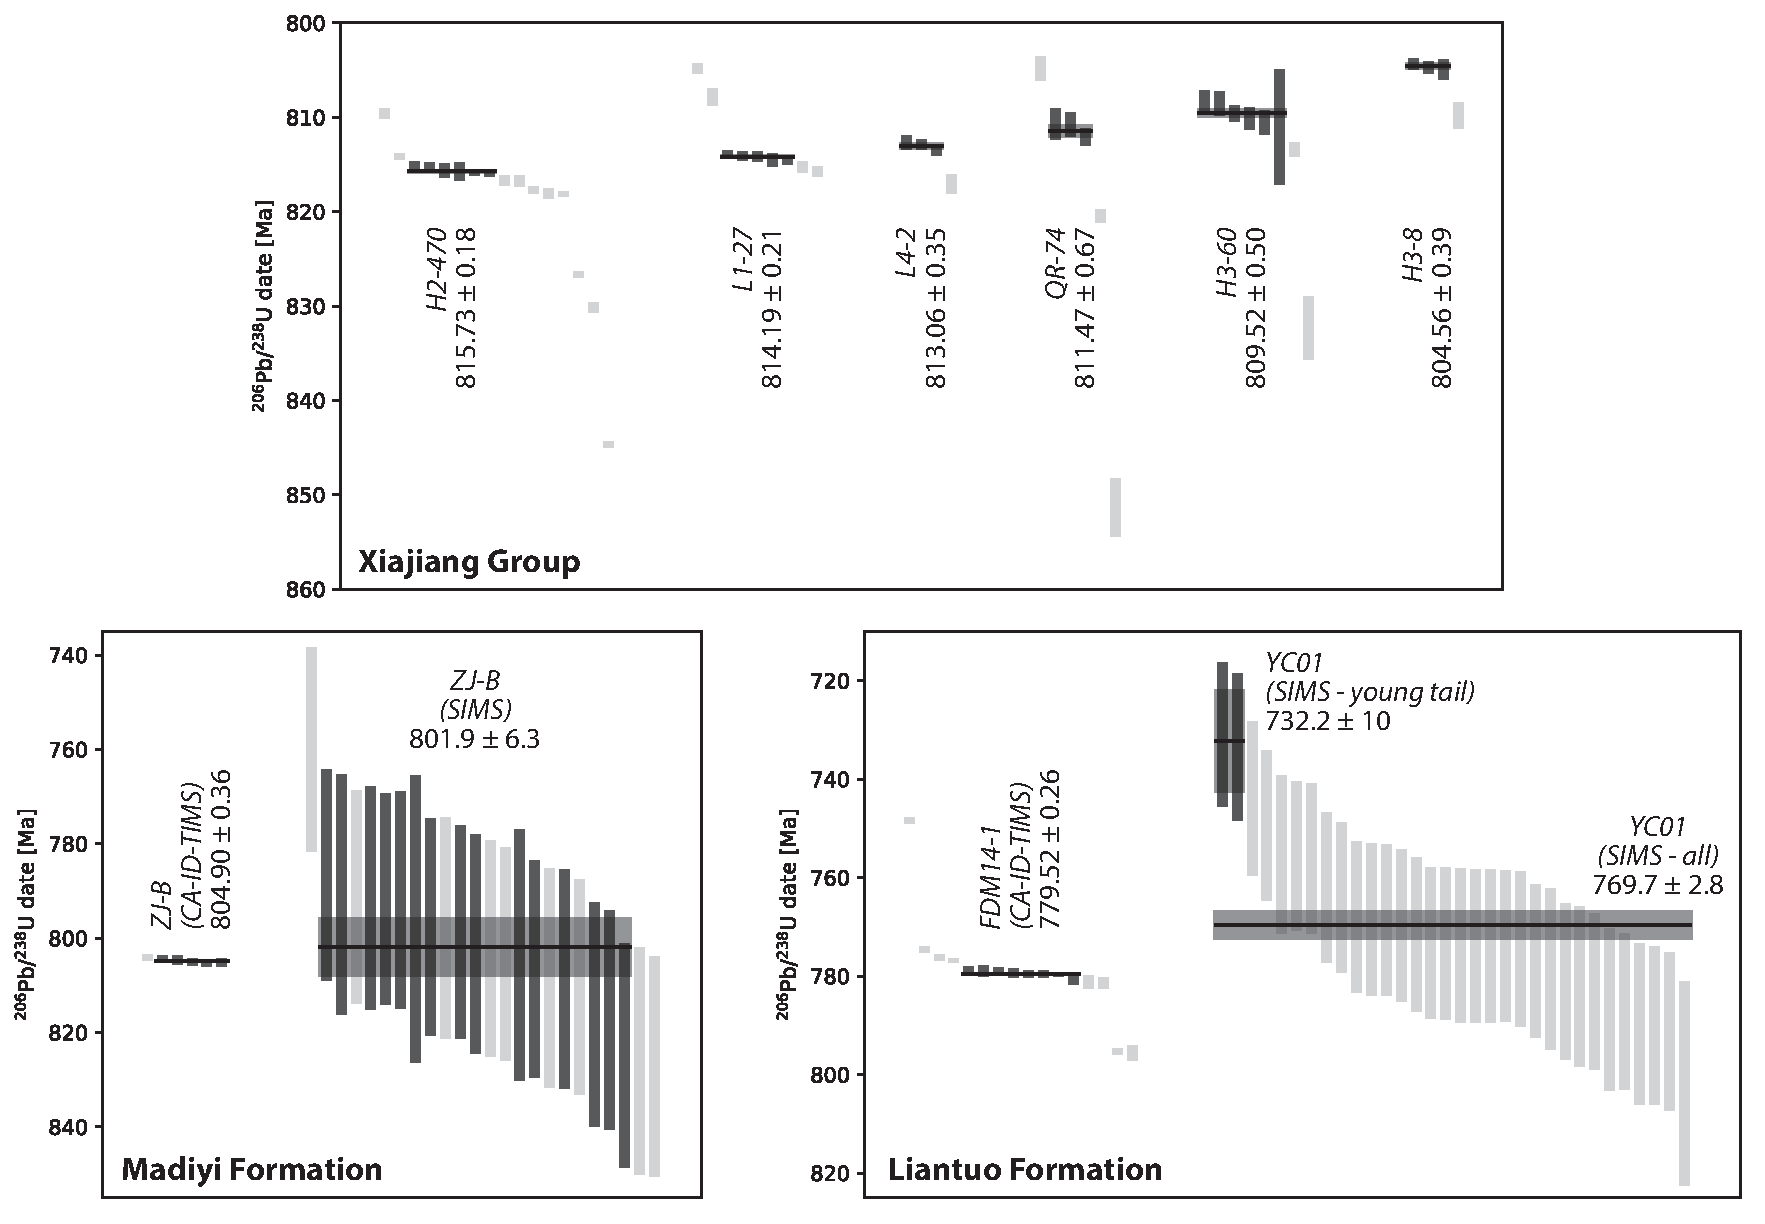
\includegraphics[width=\textwidth]{figures/Xiajiang/zircons.pdf}
    \caption[2$\sigma$ uncertainty of CA-ID-TIMS U-Pb dates for zircons analyzed in this study.]{2$\sigma$ uncertainty of CA-ID-TIMS U-Pb dates for zircons analyzed in this study. The previously reported SIMS dates for sample ZJ-B of the Madiyi Formation \citep{Xian2020a} and sample YC01 of the Liantuo Formation \citep{Lan2015a} are also shown. For sample YC01, we show the weighted mean dates that result from isolating the two youngest zircons (as is preferred in \citealp{Lan2015a}) and from including all of the zircons. Solid vertical bars indicate zircons that are included in the calculation of the weighted mean date. Faded vertical bars indicate zircons interpreted to have been inherited or affected by Pb or U loss, and are excluded in the calculation of the weighted mean date. Measurement data are and concordia diagrams are shown in the Supporting Information.}
    \label{fig:zircons}
\end{figure}

U-Pb zircon secondary ion mass spectrometry (SIMS) and laser ablation inductively coupled plasma mass spectrometry (LA-ICP-MS) analyses can be conducted relatively rapidly and are often utilized to determine the age of tuff samples. However, U-Pb determinations using SIMS are significantly less precise than that measured using CA-ID-TIMS and are subject to an U-Pb calibration correction that contributes additional uncertainty. This single data point imprecision makes it difficult to recognize real age variation within a sampled population (due to either analyses of domains with Pb loss and/or older zircon). As a result, isotope ratios measured using SIMS can be affected by Pb loss that cannot be identified at the precision of SIMS, which can bias SIMS-derived weighted mean dates toward younger ages. Conversely, deriving a weighted mean from a non-single age population (with variation not resolvable by the single data point analyses) can bias the interpreted age towards being too old. An additional issue in the interpretation of microbeam U-Pb geochronology is that there are dates in the literature where the youngest dates are deconvolved from a larger age population to derive a weighted mean that approximates the ages of eruption. Calculating a weighted mean from the `young tail' for a distribution of imprecise dates could result in a date that is too young either due to Pb loss in these grains or simply through arbitrary grouping of the youngest dates in a low precision normal distribution of dates. Such a bias could explain calculated SIMS dates from pre-Sturtian strata that are younger than ca. 717~Ma in South China (e.g. \citealp{Lan2015a}) and in practice requires other independent information to defend the interpretation. In addition to the issues surrounding age interpretations, microbeam U-Pb dates require consideration of the U/Pb calibration uncertainty that is typically 1--2\% and is a limiting uncertainty.

The chemical abrasion step of the CA-ID-TIMS method has been developed to effectively remove (i.e. leach) the analyses of radiation-damaged zones of zircon grains, which are most likely to suffer Pb loss, prior to analysis \citep{Mattinson2005a}. This technique is not perfect -- depending on the nature of the material being analysed (U content, zonation patterns), for some samples a proportion of analyses suffering Pb-loss may still persist. The higher-precision of the CA-ID-TIMS single data points often reveals age complexity with excess variance ascribed to geological age variation and residual Pb-loss.

Evaluating a hypothesis such as the Bitter Springs Stage TPW hypothesis requires precise age constraints on poles. The SIMS dates prevalent in the literature could have true age uncertainty well beyond the weighted mean uncertainty, particularly if the assumptions made are incorrect (i.e. a single age population, no Pb-loss) in addition to the calibration uncertainty. As a result, it is essential to develop CA-ID-TIMS dates in order to have high-precision age constraints on paleomagnetic poles.

We developed U-Pb CA-ID-TIMS ages from zircon for six tuff samples collected from the Xiajiang Group in the Fanjingshan region (Figs. \ref{fig:stratigraphic-sections} and \ref{fig:zircons}; Table \ref{tab:SChina-geochronology}). For each of these ash layers we make a subjective age interpretation based upon the U-Pb zircon data combined with information about the general nature of the materials. Five tuffs from the lower and middle Xiajiang Group yield dates ca. 816--810~Ma, and one tuff from near the top of the Xiajiang Group in the Hongzixi section yields a younger date of ca. 805~Ma. Within $\sim$100~m of this youngest tuff, a major unconformity separates ca. 805~Ma sediments of the Xiajiang Group with \textless717~Ma Sturtian Snowball Earth glacial deposits \citep{Bowring2007a, Macdonald2010a, MacLennan2018a, Lan2020a}.

Prior to this study, age constraints on Tonian paleomagnetic poles from the Madiyi and Liantuo formations were based on U-Pb SIMS analyses. In order to improve the precision of these age constraints, as well as evaluate whether they might be biased toward younger ages, we developed new age constraints for these poles using U-Pb CA-ID-TIMS. These new CA-ID-TIMS age constraints supersede the previous SIMS age constraints.

The tuff associated with the paleomagnetic pole for the Madiyi Formation in the Hunan province (sample ZJ-B of \citealp{Xian2020a}) is within the 12~m thick succession of the Madiyi Formation from which the paleomagnetic data were developed. A U-Pb zircon SIMS date of 801.9$\pm$6.3~Ma was reported for the tuff in \citet{Xian2020a}. The new CA-ID-TIMS data from five zircons result in a weighted mean $^{206}$Pb/$^{238}$U date of 804.90$\pm$0.36~Ma (Fig. \ref{fig:zircons}); Table \ref{tab:SChina-geochronology}). This date overlaps with the SIMS date of \citet{Xian2020a} within uncertainty and constrains the timing of the Madiyi Formation pole to higher precision.

The tuff associated with the paleomagnetic pole for the Liantuo Formation \citep{Evans2000a, Jing2015a} lies $\sim$15~m below the base of the stratigraphic interval which was sampled for paleomagnetic analysis in \citet{Evans2000a}, and is in the vicinity of a tuff that was previously dated at 748$\pm$12~Ma using SIMS (Fig. S5; \citealp{Ma1984a}). The new CA-ID-TIMS data from eight zircons result in a weighted mean $^{206}$Pb/$^{238}$U date of 779.52$\pm$0.26~Ma -- $\sim$20~m.y. older than the maximum reported uncertainty of the SIMS-derived date (Fig. \ref{fig:zircons}; Table \ref{tab:SChina-geochronology}).

\section{Discussion}

\subsection{Tectonic Setting}

The South China craton consists of two distinct tectonic blocks, the Yangtze and Cathaysia blocks, separated by the Jiangnan Orogen (Fig. \ref{fig:geologic-maps}). However, the depositional setting of sedimentary units in the Jiangnan Orogen as well as the tectonic context of the intrusive units and deformation found throughout the orogen continues to be debated in the literature. A widely-adopted model proposed that the Fanjingshan Group (and equivalent strata) was deposited in a Grenvillian (ca. 1.3--0.9~Ga) arc-related basin on the Yangtze block as the oceanic crust formerly separating the Yangtze and Cathaysia blocks subducted under the Yangtze block (e.g. \citealp{Li2002a, Li2009b}). In this model, deformation of the Fanjingshan Group was interpreted to reflect collision of the Yangtze and Cathaysia blocks as the supercontinent Rodinia came together around South China ca. 1.0--0.9~Ga, with Laurentia on the Cathaysia-side of South China and Australia on the Yangtze-side (i.e. the Missing Link model, as shown in Figure \ref{fig:Rodinia-models}). The model then proposes that later Tonian (ca. 850--750~Ma) magmatism in the Jiangnan Orogen is associated with a mantle superplume that initiated the break up of Rodinia (e.g. \citealp{Li2003a, Li2009b}). In this scenario, the Xiajiang Group (and equivalent strata) is interpreted to have been deposited within a failed intra-continental rift basin between the Yangtze and Cathaysia blocks as Australia, South China, and Laurentia rifted apart.

Geochronologic and geochemical data initially appeared to support this Missing Link model (e.g. \citealp{Li2002a, Li2003a, Li2009b}), and consequently many Neoproterozoic paleogeographic models adopted it (e.g. \citealp{Li2008a}). However, subsequent geochronologic, geochemical, and paleomagnetic data introduce new constraints that are difficult to reconcile with this model.

The timing of Yangtze and Cathaysia block collision represented by the Jiangnan Orogen can no longer be considered to be coeval with the ca. 1080 to 980~Ma Grenvillian Orogen. U-Pb LA-ICP-MS geochronologic constraints from the tuffs, sedimentary rocks, and sills of the Fanjingshan Group \citep{Zhao2011a, Wang2012d, Gao2014a} indicate that deformation of the group occurred after ca. 830~Ma. Our new U-Pb CA-ID-TIMS results constrain initiation of Xiajiang Group deposition, and therefore termination of Fanjingshan Group deformation, to have occurred by 815.73$\pm$0.18~Ma (Fig. \ref{fig:stratigraphic-sections}). The interpretation that the Jiangnan Orogeny, and the associated deformation of the Fanjingshan Group, was the result of collision between the Yangtze and Cathaysia blocks gains support from the geochemistry and geochronology of the igneous rocks of the Jiangnan Orogen that are indicative of a supra-subduction, volcanic arc setting \citep{Cawood2013a, Cawood2017a}.

The Fanjingshan Group is dominated by siliciclastic sediments and also contains horizons of volcanic rocks including pillow basalts \citep{Zhou2009a}. These units were intruded by ca. 830~Ma mafic sills with geochemical signatures consistent with subduction-related magmatism \citep{Wang2014a} as well as 835$\pm$5~Ma (U-Pb SIMS) felsic intrusive rocks (Fig. \ref{fig:geologic-maps}B; \citealp{Gao2011a}). Both fore-arc \citep{Zhao2011a} and retro/back-arc \citep{Lin2016a, Yao2019a} settings have been interpreted for the Fanjingshan Group deposition. However, fore-arc settings are typically cold and amagmatic, and consequently we prefer a syn-collisional retro-arc foreland model with ultramafic magmatism associated with slab-breakoff. In either model, the Fanjingshan Group is deposited and intruded in an arc-related basin as the oceanic crust formerly separating the Yangtze and Cathaysia blocks subducted under the Yangtze block \citep{Lin2016a}. As Yangtze and Cathaysia (or at least a portion of Cathaysia) collided between ca. 830~Ma and 815.73$\pm$0.18~Ma, sedimentary rocks of the Fanjingshan Group were folded, uplifted, and eroded. Following this deformation and the development of an erosional unconformity, subsidence enabled deposition of the overlying Xiajiang Group. Taken together, these data constrain the collision of the Yangtze and Cathaysia blocks to have occurred between ca. 830~Ma and 815.73$\pm$0.18~Ma, not ca. 1000 to 900~Ma as is proposed in the Missing Link model implemented in \citet{Li2008a}.

In addition to this evidence of Tonian convergence between the Yangtze and Cathaysia blocks, the record of the northwest Yangtze block indicates a convergent tectonic setting in the Tonian that extended into the Cryogenian. Geochronologic and geochemical constraints from the Panxi-Hannan Belt (Fig. \ref{fig:geologic-maps}) indicate that arc-related magmatism was occurring in that belt ca. 870--706~Ma \citep{Dong2012a}, and therefore that the northwestern margin of the Yangtze block was an active margin throughout the time that Rodinia is hypothesized to have been a coherent supercontinent. This arc-related magmatic activity associated with subduction along the northwestern margin of the Yangtze block is the likely source for the ashes that formed the tuffs within the Xiajiang Group that we have targeted for geochronology (Fig. \ref{fig:stratigraphic-sections}).

Finally, paleomagnetic constraints indicate that South China was at high latitudes throughout the late Tonian (discussed further in \textit{Tonian APWP of South China}) rather than at low-latitudes as would be required by the Missing Link model (discussed further in \textit{South China and Rodinia}; Fig. \ref{fig:Rodinia-models}). Additionally, the paleomagnetic data suggests that the Panxi-Hannan Belt lay from the east to the north relative to the Fanjingshan region in reconstructed coordinates during the time of Xiajiang Group deposition (ca. 815--800~Ma; Fig. \ref{fig:SChina-APWP}). At these high latitudes, the prevailing winds are polar easterlies, which is consistent with the idea that the ashes that formed the tuffs within the Xiajiang Group were transported from the Panxi-Hannan Belt \citep{Hildebrand1988a}.

Together, these constraints are inconsistent with South China being within the interior of a stable supercontinent during the Tonian. Instead, they indicate a convergent setting with the northwestern margin of the Yangtze block being an active margin into the Cryogenian rather than being juxtaposed against a conjugate continent. Therefore, the data are more compatible with South China on the periphery of Rodinia or disconnected from it entirely (Fig. \ref{fig:Rodinia-models}).

The tectonic setting of the basin in which the Xiajiang Group (and equivalent strata) was deposited is commonly interpreted as a failed intra-continental rift basin \citep{Zhang2019c}, potentially associated with the hypothesized mantle superplume that initiated the break up of Rodinia \citep{Li2003a, Li2009b}. However, this basin development framework is rooted in a tectonic setting interpretation that would have South China within the interior of a supercontinent undergoing break-up --- a setting that is inconsistent with available constraints. Rather, any basin development model needs to honor the following:

\begin{itemize}
    \item There was a geologically short interval (ca. 15~m.y.) between the orogenesis that deformed the Fanjingshan Group and the subsidence that enabled deposition of the Xiajiang Group.
    \item There was an active margin along the northwestern margin of the Yangtze block at the time of Xiajiang Group subsidence. This margin is the likely source of the tuffs throughout the Xiajiang Group stratigraphy.
    \item The site of Xiajiang Group deposition must have been folded, uplifted, and eroded prior to subsidence.
    \item Subsidence rates were initially quite high as evidenced by the rapid sediment accumulation rates in the Xiajiang Group. These high subsidence rates led to the deep-water setting of the Xiajiang Group sediments.
    \item While some strata could be missing through glacial erosion, the duration of missing time ($\sim$90~m.y.) in the ca. 805 and 717~Ma pre-Sturtian unconformity suggests limited sediment accumulation in the pre-Sturtian interval relative to the thick ca. 815 to 805~Ma succession.
\end{itemize}

The Nanhua Basin into which the Xiajiang Group was deposited formed inland from the Panxi-Hannan Belt \citep{Cawood2017a}. Based on the interpretation that the Panxi-Hannan Belt was an active arc at the time of Xiajiang Group deposition, \citet{Qi2019a} argued that Nanhua Basin formation was the result of back-arc extension. Importantly, the timing of deposition of the Xiajiang Group coincides with the initiation of  back-arc extension in the Panxi-Hannan arc \citep{Dong2012a}. Back-arc extension provides a mechanism to explain regional extension and subsidence in the region of the Jiangnan suture. Furthermore, given that back-arc basin formation is the result of the combined driving mechanisms of surface kinematics and dynamic mantle flow \citep{Sdrolias2006a}, it can lead to both rapid and transient subsidence. Geologic observations in more recent back-arcs have been interpreted to indicate significant back-arc extension in regions where lithosphere has been thickened through orogenesis \citep{Gogus2015a}. Numerical modeling has shown that post-orogenic lithosphere removal (such as that occurring as a result of delamination) in continental back-arc settings can lead to large-scale subsidence \citep{Gogus2015a}. This mechanism could explain the transition at the site of Xiajiang Group deposition from folding, uplift, and erosion in the Jiangnan Orogen as Yangtze collided with Cathaysia between ca. 830~Ma and 815.73$\pm$0.18~Ma, to Nanhua Basin subsidence as a back-arc basin formed. The Nanhua Basin is therefore best interpreted as a polyphase basin wherein this Tonian subsidence was followed by Cryogenian and Ediacaran subsidence potentially as the result of other mechanisms. The tuffs found throughout the Xiajiang Group stratigraphy are the result of the arc on the northwestern margin of the Yangtze block that was active throughout deposition, both driving subsidence through back-arc extension and contributing ashes via the prevailing polar easterly winds that enable us to develop geochronologic constraints.

\subsection{Tonian APWP of South China}

\begin{table}[h!]
\caption[Neoproterozoic paleomagnetic poles for South China.]{Neoproterozoic paleomagnetic poles for South China.}
\vspace{0.25cm}
\resizebox{\linewidth}{!}{
	\begin{tabular}{lllccccccllc}
	\hline
	\textbf{pole} & \textbf{nominal age (Ma)} & \textbf{age method} & \textbf{site lat.} & \textbf{site lon.} & \textbf{pole lat.} & \textbf{pole lon.} & \textbf{A$_{95}$} & \textbf{f} & \textbf{pole ref.} & \textbf{age ref.} & \textbf{note} \\\\
	Yanbian dikes & 824$\pm$6 & SIMS & 26.9 & 101.5 & 45.1 & 130.4 & 19.0 & 1.0 & \citet{Niu2016a} & \citet{Niu2016a} & (2) \\
    Xiaofeng dikes & 821.64$\pm$0.2 & CA-ID-TIMS & 31.0 & 111.2 & 26.1 & 82.1 & 14.6 & 1.0 & \citet{Jing2019a} & \citet{Wang2016b} & (3) \\
    Xiajiang Group & 816--810 & CA-ID-TIMS & 27.9 & 108.8 & 42.7 & 104.0 & 8.1 & 0.6 & this study & this study & - \\
	Madiyi Formation & 804.90$\pm$0.99 & CA-ID-TIMS & 27.5 & 109.6 & 34.7 & 82.0 & 6.7 & 0.6 & \citet{Xian2020a} & this study & (4) \\
    Chengjiang Formation & 799.5$\pm$8.4 & SIMS & 25.1 & 102.4 & 29.7 & 75.3 & 7.9 & 0.6 & \citet{Jing2019a} & \citet{Jing2019a} & (5) \\
    Liantuo Formation & $\leq$779.52$\pm$0.92 & CA-ID-TIMS & 30.8 & 111.1 & 19.6 & 144.4 & 4.2 & 0.6 & \citet{Jing2015a} & this study & (5) \\
	\hline
	\end{tabular}}

\scriptsize
\flushleft \emph{Notes:} \\
(1) \textbf{f} is the flattening factor, where f=1 indicates no inclination shallowing and f=0 indicates a completely flattened direction.\\
(2) Located within mobile belt.\\
(3) Pole recalculated after \citet{Li2004a}.\\
(4) Pole converted from specimen to site mean in this study.\\
(5) Pole converted from specimen to site mean and inclination correction applied in this study.\\
\label{tab:South-China-poles}
\end{table}

\begin{figure}[h!]
    \centering
    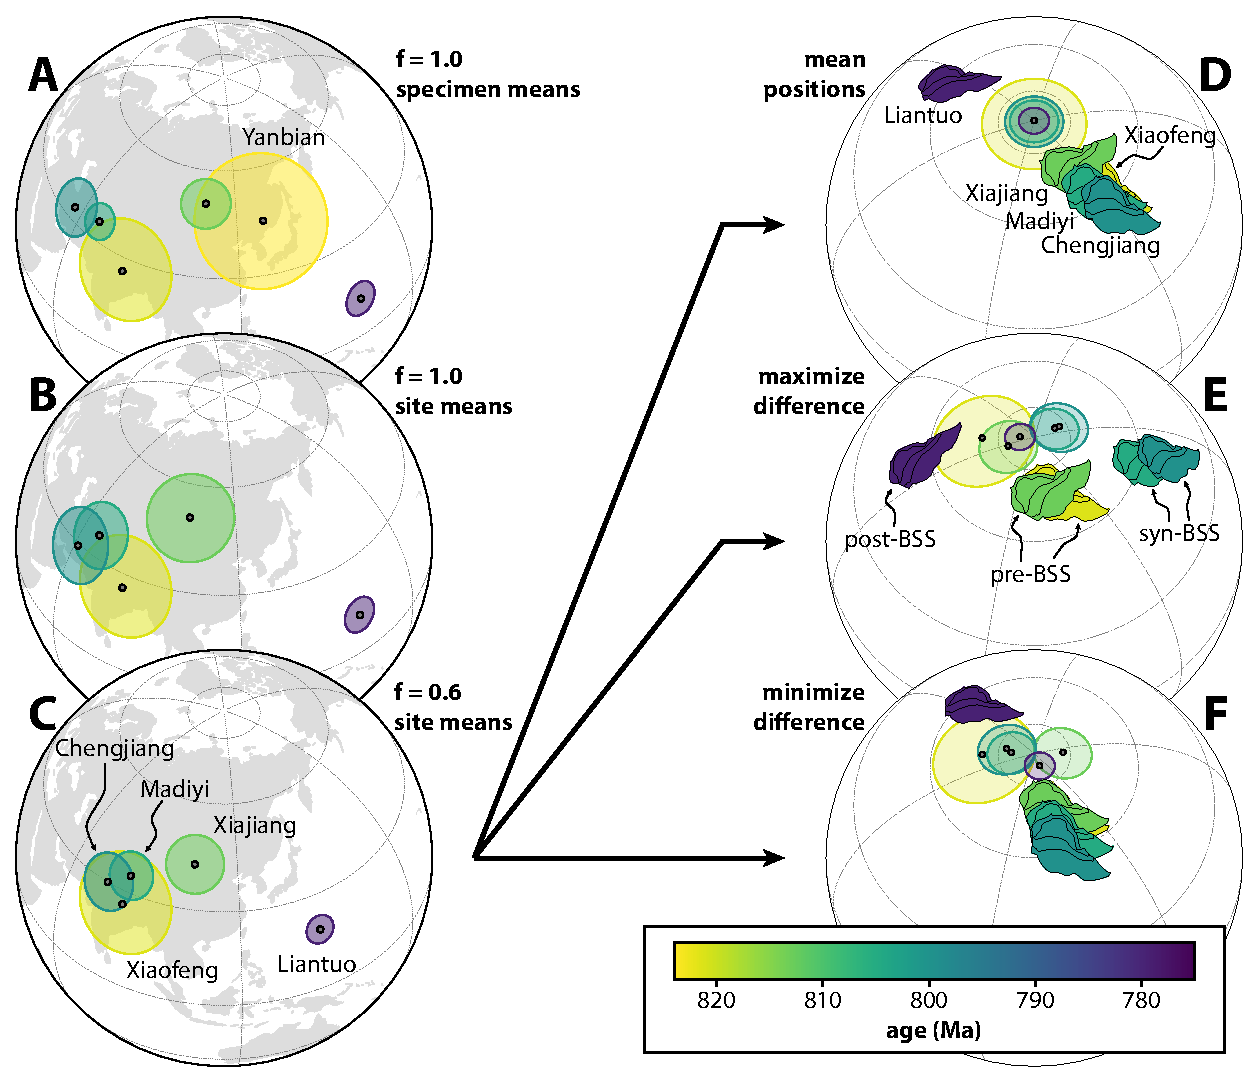
\includegraphics[width=\textwidth]{figures/Xiajiang/SChina-APWP.pdf}
    \caption[Tonian apparent polar wander paths and paleogeographic models for South China.]{Tonian apparent polar wander paths (APWPs) and paleogeographic models for South China. \textbf{A)} APWP using all available paleomagnetic poles. Both the original \citep{Li2004a} and recalculated \citep{Jing2019a} Xiaofeng dikes poles are shown. Poles derived from sedimentary rocks are shown as specimen means without an inclination correction (Table \ref{tab:South-China-poles}). \textbf{B)} APWP excluding the Yanbian dikes and original Xiaofeng dikes poles. Poles derived from sedimentary rocks are shown as site means without an inclination correction. \textbf{C)} Our preferred APWP excluding the Yanbian dikes and original Xiaofeng dikes poles, and using site mean poles from sedimentary rocks with an inclination correction ($f=0.6$). \textbf{D)} Paleogeographic model based on the preferred APWP in C. South China is reconstructed using the means of the poles. \textbf{E)} Paleogeographic model based on the preferred APWP with South China reconstructed to maximize the difference in position between the pre-, syn-, and post-Bitter Springs Stage (BSS) poles as permitted by the A$_{95}$ uncertainties. \textbf{F)} Paleogeographic model based on the preferred APWP with South China reconstructed to minimize the difference in position permitted by the A$_{95}$ uncertainties of all poles.}
    \label{fig:SChina-APWP}
\end{figure}

With the exception of the highest ash sample in the Hongzixi section, all dated ash samples from the Xiajiang Group of the Fanjingshan region yield an age of ca. 816--810~Ma (Fig. \ref{fig:stratigraphic-sections}). Furthermore, the high temperature components in all sites record similar directions (Fig. \ref{fig:site-means}). We therefore take the parsimonious interpretation that variability in the high temperature component between specimens/sites is largely recording short time-scale secular variation in the magnetic field, and therefore develop a single paleomagnetic pole from the mean direction of the high temperature component from all sites (Fig. \ref{fig:site-means}). Based on the geochronologic constraints (Fig. \ref{fig:stratigraphic-sections}), we assign a nominal age to this pole of 813$\pm$3~Ma. However, we discuss the possibility of multiple poles being recorded in the Xiajiang Group below.

This new pole can be combined with existing Neoproterozoic paleomagnetic poles for South China (summarized in Table \ref{tab:South-China-poles}) to develop an apparent polar wander path (APWP). There are complications associated with the interpretation of these poles and their assigned ages and we will discuss each in turn.

The Yanbian dikes pole \citep{Niu2016a} was obtained from a deformed region on the western-most margin of the South China craton that experienced vertical axis rotation during the Cenozoic collision of India with Asia. The magnitude of this vertical axis rotation was estimated to be 5.3$\pm$3.0\degrees based on paleomagnetic data from Pliocene sedimentary rocks in the region \citep{Zhu2008a}, and \citet{Niu2016a} applied a 5\degrees vertical axis rotation correction to their Yanbian dikes pole. However, the vertical axis rotation correction may be as little as 2.3\degrees or as high as 8.3\degrees at the 95\% confidence level \citep{Zhu2008a}. The Yanbian dikes may also have experienced pre-Pliocene vertical axis rotation. Furthermore, no tilt-correction was applied to the majority of the directions obtained from the Yanbian dikes, despite observations that the dikes exhibit dips that range from 43\degrees to vertical \citep{Niu2016a}. Finally, the Yanbian dikes pole is inconsistent with the Xiaofeng dikes pole (Fig. \ref{fig:SChina-APWP}A) despite the similar age of these two poles. Given these complications, we exclude the Yanbian dikes pole as a constraint in our preferred Tonian South China APWP (Fig. \ref{fig:SChina-APWP}C).

The Xiaofeng dikes pole has had both its direction and age revised since its initial publication in \citet{Li2004a}. \citet{Jing2019a} recognized that a subset of the dikes that were used to obtain the Xiaofeng dikes pole are located between two faults and have paleomagnetic directions that may have been rotated relative to the rest of the dikes. Therefore, to account for the possibility of vertical axis rotation affecting this subset of dikes, \citet{Jing2019a} recalculated the Xiaofeng dikes pole by excluding them. The resulting pole is closer to the other ca. 820-800~Ma poles for South China (Fig. \ref{fig:SChina-APWP}), although further work is needed to substantiate whether this difference in pole position is robust. In addition, the Xiaofeng dikes were originally dated to 802$\pm$10~Ma based on U-Pb SIMS analyses on zircon from the dikes \citep{Li2004a}. When zircon from these dikes were reanalyzed at higher precision using CA-ID-TIMS, their age was revealed to be significantly older (821.64$\pm$0.2~Ma; \citealp{Wang2016b}). This revised age constraint for the Xiaofeng dikes pole is utilized here (Table \ref{tab:South-China-poles}; Fig. \ref{fig:SChina-APWP}).

The previous age constraint on the Madiyi Formation pole of 801.9$\pm$6.3~Ma was also developed using U-Pb SIMS measurements on zircon from a tuff within the section where the paleomagnetic data were developed \citep{Xian2020a}. Our new CA-ID-TIMS date of 804.90$\pm$0.36~Ma is within the uncertainty of this SIMS date and provides a higher precision age constraint on the age of the pole (Fig. \ref{fig:zircons}) which supersedes the previous age and is utilized here (Table \ref{tab:South-China-poles}; Fig. \ref{fig:SChina-APWP}).

The paleomagnetic pole for the upper Liantuo Formation has long been an important constraint for the Neoproterozoic paleogeography of South China \citep{Evans2000a}. The Liantuo Formation unconformably overlies the Huangling granite suite for which U-Pb SIMS dates of 863$\pm$9, 844$\pm$10, and 842$\pm$10~Ma have been developed \citep{Wei2012a}. These granites are intruded by the 821.64$\pm$0.2~Ma Xiaofeng dikes \citep{Wang2016b}. The Liantuo Formation is unconformably overlain by Cryogenian glacial deposits. The age assigned to the Liantuo Formation pole has varied in the literature. When a paleomagnetic pole from the formation was first reported in \citet{Evans2000a}, it was assigned an age of 748$\pm$12~Ma based on an U-Pb SIMS date on a tuff $\sim$15~m below the base of the stratigraphic interval that was sampled for paleomagnetic analysis (\citealp{Ma1984a}; Fig. S5). When this paleomagnetic pole was updated in \citet{Jing2015a} with the addition of paleomagnetic data from additional sites to the southwest of the stratigraphic section sampled in \citet{Evans2000a}, its age was interpreted to be ca. 720~Ma based on U-Pb SIMS dates on tuffs within the upper 20~m of the Liantuo Formation across the Three Gorges Area \citep{Lan2015a}. A challenge with these U-Pb SIMS dates is that there is a distribution of dated grains around a peak of ca. 780 to 770~Ma that includes sparse younger dates (Fig. \ref{fig:zircons}; \citealp{Lan2015a}). In \citet{Lan2015a}, these younger dates are interpreted as the eruptive age of the tuffs, but it is possible that these grains are biased young. Ambiguity associated with correlation of the Liantuo Formation with possibly equivalent stratigraphy adds further complexity to the interpretation of geochronologic constraints on the Liantuo Formation. For example, zircons from a tuffaceous siltstone $\sim$25~m below Sturtian glacial deposits in the Gongdong Formation of northern Guangxi, which is often interpreted to be a deeper water equivalent to the Liantuo Formation \citep{Wang2003a, Pi2016a}, yield a weighted mean CA-ID-IRMS date of 720.16$\pm$1.40~Ma \citep{Lan2020a}. If this interpretation that the Gongdong Formation correlates to the Liantuo Formation is correct, it suggests that, at least in some parts of the Nanhua Basin, sediments as young as ca. 720~Ma are preserved. On the other hand, if the two formations are not correlative, then the CA-ID-IRMS date of 720.16$\pm$1.40~Ma \citep{Lan2020a} does not place any geochronologic constraints on the Liantuo Formation.

We have developed a new CA-ID-TIMS date of 779.52$\pm$0.26~Ma for a tuff in the Liantuo Formation at the same location studied by \citet{Ma1984a} close to the section sampled for paleomagnetic analyses by \citet{Evans2000a}. Similar to the updated Xiaofeng dikes geochronology, this date is appreciably older than interpretations based on the previous SIMS U-Pb dates. It is possible that some or all of the zircons included in the calculation of the weighted mean date may be detrital and not representative of the eruptive age of the tuff. However, the consistency of the zircon dates (Fig. \ref{fig:zircons}) suggests that the weighted mean date likely represents an eruptive age. Furthermore, while the $\sim$15~m of stratigraphy between the tuff and the paleomagnetic data of \citet{Evans2000a} could represent significant time, the similar lithologies throughout the interval (fine to medium sandstone interbedded with siltstone; Fig. S5) suggests conformable deposition. Therefore, the age of the tuff is likely to be similar in age to the sedimentary rocks from which the paleomagnetic data were derived and unlikely to be tens of millions of years older. However, without further high-precision geochronologic constraints from the Liantuo Formation at or above the stratigraphy from which the paleomagnetic pole was derived, the possibility remains that the Liantuo Formation paleomagnetic pole post-dates 779.52$\pm$0.26~Ma. We prefer the interpretation that the age of the Liantuo Formation and its pole is close to 780~Ma and that the Liantuo Formation is not correlative to the ca. 720~Ma Gongdong Formation, which is preserved conformably below Cryogenian glacial deposits in a deeper-water setting \citep{Lan2020a}.

The existing date of 799.5$\pm$8.4 Ma for the Chengjiang Formation pole was also developed using SIMS (Table \ref{tab:South-China-poles}). As evidenced for the Xiaofeng dikes and the Liantuo Formation, when SIMS-derived ages are re-investigated through CA-ID-TIMS, the result can be a significantly different date. Therefore, the accuracy of the SIMS-derived dates for the Chengjiang Formation pole remains uncertain.

The Xiajiang Group paleomagnetic pole developed in this study is calculated as a site mean (i.e. the mean of the means of specimen directions for each site; Fig. \ref{fig:site-means}). However, the Chengjiang and Madiyi poles are reported in \citet{Jing2019a} and \citet{Xian2020a} as specimen means (i.e. the mean of specimen directions across all sites). While both methods can be justified for sedimentary rocks, the specimen mean direction leads to paleomagnetic poles with smaller $A_{95}$ uncertainty ellipses due to the larger number of directions used to obtain the mean which has the potential to underestimate the uncertainty. We recalculate the paleomagnetic poles for the Chengjiang and Madiyi formations as site means, to be consistent with the methodology used to develop our Xiajiang Group pole (Figs. \ref{fig:SChina-APWP}B and \ref{fig:SChina-APWP}C).

An inclination correction has been applied to the paleomagnetic pole obtained from the Xiajiang Group in this study. Similarly, an inclination correction was applied to the pole obtained from the Madiyi Formation \citep{Xian2020a}. Given that the poles from the Chengjiang and Liantuo formations are also derived from the hematite-held magnetization of similar siliciclastic sedimentary rocks, we apply the same inclination correction ($f=0.6$) to these poles as that applied to the Xiajiang Group and Madiyi Formation poles (Fig. \ref{fig:SChina-APWP}C). Given potential variability in inclination shallowing, the flattening could vary from this value which is an additional source of uncertainty.

The Xiaofeng dikes and the inclination-corrected Madiyi and Chengjiang poles all overlap within uncertainty, and the Xiajiang Group records a distinct, but similar, position as well (Fig. \ref{fig:SChina-APWP}). Together, these poles constrain South China to have been in a roughly stable position at high latitudes ($\gtrsim$60\degrees) ca. 820--800~Ma (Figs. \ref{fig:SChina-APWP} and \ref{fig:centroid-paleolatitudes}). The Liantuo Formation pole also constrains South China to be at high latitudes, although with a different orientation to the ca. 820--800~Ma position (Figs. \ref{fig:SChina-APWP} and \ref{fig:centroid-paleolatitudes}). The poles constrain South China to be at high latitudes in the latter half of the Tonian, likely drifting across the pole after ca. 805~Ma (Fig. \ref{fig:SChina-APWP}).

\subsection{South China and Rodinia}

\begin{table}[h!]
\caption[900-700~Ma paleomagnetic poles for cratons proximal to South China.]{900-700~Ma paleomagnetic poles for cratons proximal to South China.}
\vspace{0.25cm}
\resizebox{\linewidth}{!}{
	\begin{tabular}{lcccccclc}
	\hline
	\textbf{pole} & \textbf{nominal age (Ma)} & \textbf{site lat.} & \textbf{site lon.} & \textbf{pole lat.} & \textbf{pole lon.} & \textbf{A$_{95}$} & \textbf{ref.} & \textbf{grade} \\
	&&&&&&&& \\
	\textbf{Laurentia} &&&&&&&& \\
	Gunbarrel dikes & 778$^{+2}_{-2}$ & 44.8 & 248.7 & 9.1 & 138.2 & 12.0 & \citet{Eyster2019a} & B \\
	Uinta Mountain Group & 760$^{+6}_{-10}$ & 40.8 & 250.7 & 0.8 & 161.3 & 4.7 & \citet{Weil2006a} & B \\
	Carbon Canyon & 757$^{+7}_{-7}$ & 36.1 & 248.2 & -0.5 & 166 & 9.7 & \citet{Eyster2019a} & NR \\
	Carbon Butte/Awatubi & 751$^{+8}_{-8}$ & 35.2 & 248.5 & 14.2 & 163.8 & 3.5 & \citet{Eyster2019a} & NR \\
	Franklin event grand mean & 724$^{+3}_{-3}$ & 73.0 & 275.4 & 6.7 & 162.1 & 3.0 & \citet{Denyszyn2009a} & A \\
	&&&&&&&& \\
	\textbf{Svalbard} &&&&&&&& \\
	Lower Grusdievbreen Formation & 815$^{+5}_{-5}$ & 79.0 & 18.0 & 19.6 & 204.9 & 10.9 & \citet{Maloof2006a} & B \\
	Upper Grusdievbreen Formation & 802$^{+8}_{-7}$ & 78.9 & 18.2 & -1.1 & 252.6 & 6.2 & \citet{Maloof2006a} & B \\
	Svanbergfjellet Formation & 785$^{+5}_{-5}$ & 78.5 & 18.0 & 25.9 & 226.8 & 5.8 & \citet{Maloof2006a} & B \\
	&&&&&&&& \\
	\textbf{Siberia} &&&&&&&& \\
	Kitoi Cryogenian dikes & 758$^{+4}_{-4}$ & 52.3 & 102.8 & 1.1 & 21.8 & 5.6 & \citet{Pisarevsky2013a} & A \\
	&&&&&&&& \\
	\textbf{Australia} &&&&&&&& \\
	Browne Formation & 855$^{+45}_{-45}$ & -25.0 & 123.8 & 44.5 & 141.7 & 6.8 & \citet{Pisarevsky2007a} & B \\
	Johnny's Creek siltstones & 760$^{+30}_{-30}$ & -24.0 & 133.5 & 15.8 & 83.0 & 13.5 & \citet{Swanson-Hysell2012a} & B \\
	Mundine Well dikes combined & 755$^{+3}_{-3}$ & -25.5 & 115.0 & 45.3 & 135.4 & 4.1 & \citet{Wingate2000a} & A \\
	&&&&&&&& \\
	\textbf{India} &&&&&&&& \\
	Malani Igneous Suite combined & 752$^{+18}_{-18}$ & 25.3 & 72.6 & 69.4 & 78.6 & 6.0 & \citet{Meert2013a} & A \\
	\hline
	\end{tabular}}

\scriptsize
\flushleft \emph{Notes:} \\
(1) \textbf{grade} is the quality of the pole as assessed by the Nordic Paleomagnetism Workshops \citep{Evans2021a}. `A' refers to poles that are considered to provide essential constraints given their high quality. `B'
refers to poles that are likely high quality, but retain some ambiguity about their age or direction. `NR' refers to poles that were not rated at the Nordic Paleomagnetism Workshops. \\
\label{tab:other-poles}
\end{table}

\begin{figure}[h!]
    \centering
    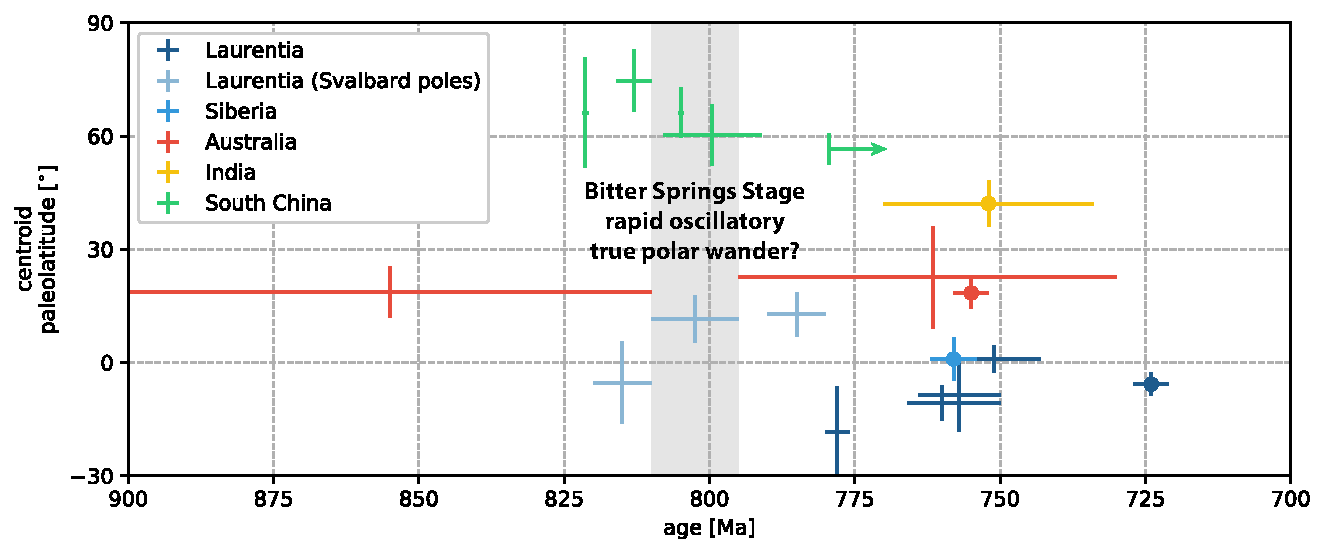
\includegraphics[width=\textwidth]{figures/Xiajiang/centroid-paleolatitudes.pdf}
    \caption[Paleolatitudes of points in the center of South China and other cratons implied by available paleomagnetic poles.]{Paleolatitudes of points in the center of South China and other cratons implied by available paleomagnetic poles shown with age and paleolatitude uncertainty (Tables \ref{tab:South-China-poles} and \ref{tab:other-poles}). The light blue `Laurentia (Svalbard poles)' are for the centroid of Laurentia reconstructed using Svalbard poles with Svalbard rotated back to Laurentia. Points with a circle in the center indicate paleomagnetic poles that were given an `A' rating by the Nordic Paleomagnetism Workshops. The grey bar indicates the timing of the ca. 810-795~Ma Bitter Springs Stage which is hypothesized to have been bracketed by rapid true polar wander rotations.}
    \label{fig:centroid-paleolatitudes}
\end{figure}

\begin{figure}[h!]
    \centering
    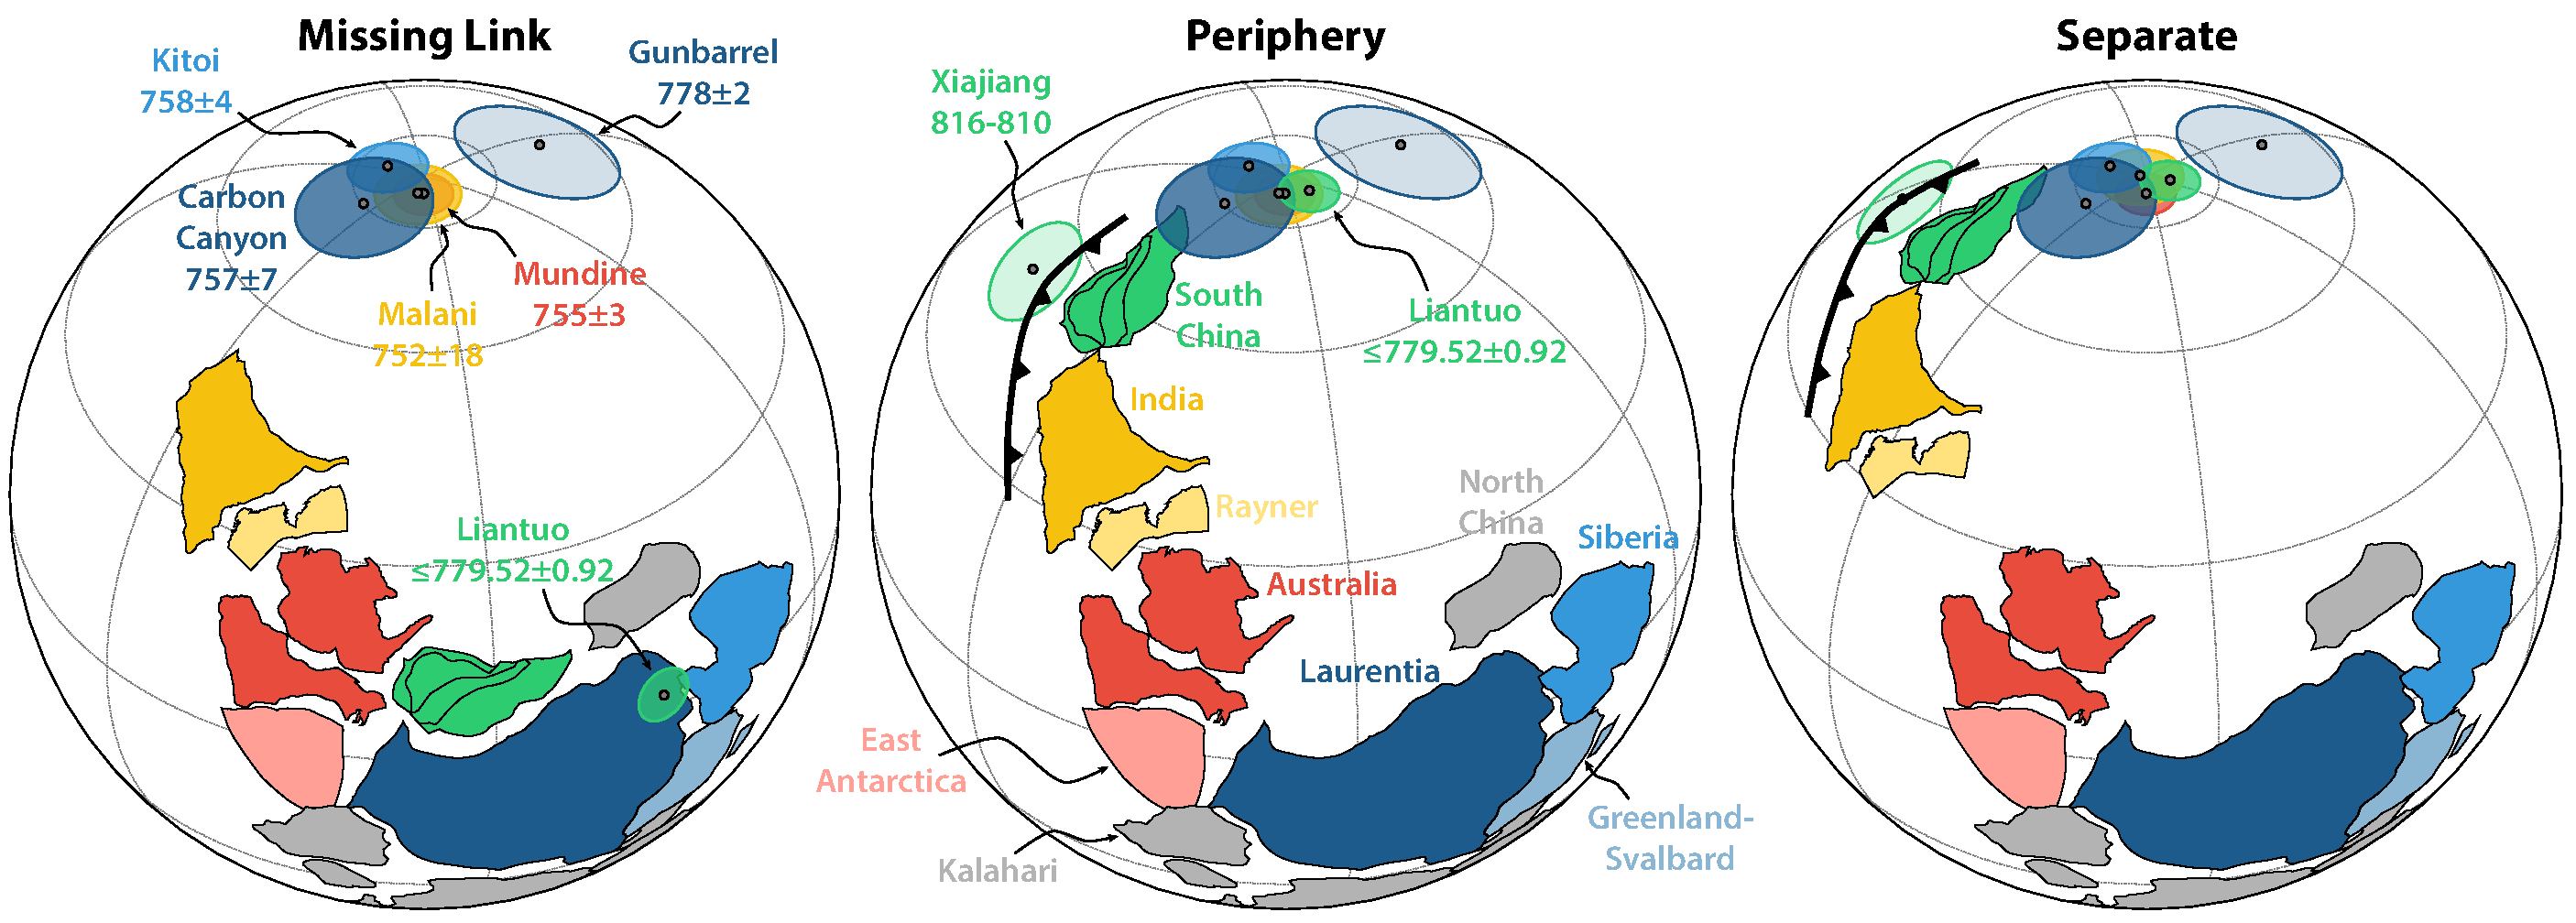
\includegraphics[width=\textwidth]{figures/Xiajiang/Rodinia-models.pdf}
    \caption[Paleogeographic reconstructions for Rodinia at 755~Ma.]{Paleogeographic reconstructions for Rodinia at 755~Ma. The Missing Link model places South China at low latitudes between Australia and Laurentia, which is inconsistent with both the paleomagnetic data as well as the tectonic context of South China. The Periphery model instead places South China at high latitudes connected to India, which satisfies the ca. 755~Ma and 780~Ma paleomagnetic data and allows for an active margin along the Panxi-Hannan Belt at this time. In order to satisfy ca. 821-805~Ma paleomagnetic data from South China, anticlockwise rotation of the entire Rodinia supercontinent from ca. 821-805~Ma to ca. 780~Ma is required in this Periphery model. The Separate model disconnects South China-India-Rayner from Rodinia. The Euler rotation parameters for South China relative to India in the Periphery and Separate models are (6.72\degrees N, 77.69\degrees E, 67.96\degrees). Blocks that are not directly relevant to the relationship between South China and Rodinia are shown in grey.}
    \label{fig:Rodinia-models}
\end{figure}

Connections between Siberia \citep{Ernst2016a, Evans2016a}, Australia-East Antarctica \citep{Veevers1988a, Duebendorfer2002a, Goodge2008a, Goodge2010a, Li2011a, Swanson-Hysell2012a, Eyster2019a}, and the western margin of Laurentia are reasonably well-established for the late Tonian (Fig. \ref{fig:Rodinia-models}). Paleomagnetic poles from India ca. 1070 and 750~Ma permit a connection with northwest Australia through the Tonian \citep{Swanson-Hysell2012a}, although it has also been suggested that India was disconnected from Rodinia during this time \citep{Merdith2017a}. Within this paleogeographic context of northern Rodinia, three models of South China's relationship with Rodinia have been proposed, which we refer to as the ``Missing Link,'' ``Periphery,'' and ``Separate'' models (Fig. \ref{fig:Rodinia-models}). The Missing Link model proposes that the supercontinent Rodinia came together around South China ca. 1.0--0.9~Ga, with Laurentia on the Cathaysia-side of South China and Australia on the Yangtze-side (Fig. \ref{fig:Rodinia-models}). The model was initially proposed to reconcile mismatches in the Mesoproterozoic geology of Australia-East Antarctica and Laurentia \citep{Li1995a}. However, paleomagnetic data from South China constrain it to be at high latitudes from ca. 821~Ma to at least 780~Ma (\textit{Tonian APWP of South China}, Fig. \ref{fig:SChina-APWP}), whereas paleomagnetic data from Australia, Laurentia, and Siberia all constrain Rodinia to be on or near the equator ca. 775~Ma (Figs. \ref{fig:centroid-paleolatitudes} and \ref{fig:Rodinia-models}). Furthermore, as previously discussed, the tectonic context of South China, with collision between the Yangtze and Cathaysia blocks between ca. 830~Ma and 815.73$\pm$0.18~Ma and subduction along northwestern Yangtze ca. 870-706~Ma (\textit{Tectonic Setting}), cannot be reconciled with a position of South China within the interior of a stable supercontinent anytime in the Tonian Period.

On the other hand, the Periphery model (Fig. \ref{fig:Rodinia-models}) is consistent with both the paleomagnetic constraints as well as our current understanding of the tectonic context of South China. In our Periphery model configuration, South China is at high latitudes, connected to Rodinia via northwestern India. Yangtze is free to have travelled across an open ocean to collide with Cathaysia between ca. 830~Ma and 815.73$\pm$0.18~Ma. Northwestern Yangtze faces this open ocean, allowing for subduction along that margin in the Tonian and into the Cryogenian. Tonian volcanism in northwest India shares geochemical characteristics with arc magmatism in the Panxi-Hannan Belt \citep{Ashwal2013a, Cawood2017a}, which has been interpreted as the result of a continuous subduction zone along northwestern Yangtze and western India and consistent with a connection between western South China and northwestern India. Detrital zircon spectra of Cryogenian sediments in South China also appear similar to that observed in northwestern India, further supporting this connection \citep{Cawood2017a, Qi2020a}. However, the ca. 755~Ma paleomagnetic poles result in a Periphery model configuration that differs from the paleogeographic models proposed in the literature that also place South China along the periphery of Rodinia. For example, it has been proposed that India-South China was connected to Rodinia, but further south along the western margin of Rodinia such that eastern India was juxtaposed against western East Antarctica and eastern South China was juxtaposed against western Australia \citep{Cawood2017a}. However, ca. 755~Ma paleomagnetic poles from South China, India, and Australia are inconsistent with this alternative position.

It has also been proposed that India-South China was disconnected from Rodinia entirely \citep{Merdith2017a}. In this Separate model, the Rayner province is also interpreted to be a terrane disconnected from Rodinia that amalgamated with India ca. 900~Ma resulting in the Eastern Ghats Orogen in eastern India, with subduction continuing along Rayner's margin until India-Rayner collides with East Antarctica near the Precambrian-Cambrian boundary \citep{Merdith2017a}. In contrast, other models of Rodinia interpret Rayner to have been part of Rodinia by 900~Ma, and that the Eastern Ghats Orogen records amalgamation of India with Rodinia \citep{Li2008a}. Current geologic constraints from Rayner do not differentiate between these two scenarios.

Importantly, paleomagnetic data indicate that South China drifted across the pole after ca. 800~Ma (Fig. \ref{fig:SChina-APWP}). In order to satisfy these paleomagnetic constraints, the Periphery model in which South China is in a constant position relative to the core of Rodinia would need to call upon anticlockwise vertical axis rotation of the entire Rodinia supercontinent(Fig. \ref{fig:Rodinia-models}). Furthermore, the Periphery model would imply that the Lower and Upper Grusdievbreen Formation poles from Svalbard are inconsistent with the paleomagnetic data from South China, and therefore require that the Svalbard poles cannot be interpreted as robust ca. 800~Ma paleomagnetic constraints on the configuration and orientation of Rodinia. On the other hand, the Separate model does not require rotation of Rodinia to satisfy the paleomagnetic constraints from South China, and could allow the Svalbard poles to be reconciled with the South China poles.

\subsection{Bitter Springs Stage True Polar Wander}

TPW should result in the same change in paleomagnetic pole positions for all continents. As a result, the Bitter Springs Stage TPW hypothesis predicts a $\sim$50\degrees change in pole position between pre-Bitter Springs Stage poles (\textgreater ca. 810~Ma) and syn-Bitter Springs Stage poles (ca. 810 to 795~Ma), with a similar angular difference between syn-Bitter Springs Stage poles and post-Bitter Springs Stage poles (\textless ca. 795~Ma).

Paleomagnetic data from the Xiajiang Group of the Fanjingshan region have the potential to test this hypothesis. Our U-Pb dates demonstrate that there are Xiajiang Group sedimentary rocks that are both older and younger than the onset of the Bitter Springs Stage (ca. 810~Ma) preserved in at least some parts of the Fanjingshan region (Fig. \ref{fig:stratigraphic-sections}). The bulk of the high temperature component paleomagnetic data (11 of 15 sites) were developed from strata below tuffs that are dated to be \textgreater 810~Ma, and are therefore unambiguously constrained to have been deposited prior to the Bitter Springs Stage. However, the remaining 4 sites could have been deposited during the Bitter Springs Stage. One site that yielded a stable and consistent high temperature component in the Hongzixi section is bracketed by tuffs that constrain it to be between 809.52$\pm$0.50~Ma and 804.56$\pm$0.39~Ma (Fig. \ref{fig:stratigraphic-sections}). However, this site cannot be interpreted to have been deposited during the Bitter Springs Stage, since the onset of the Bitter Springs Stage can only be constrained to have occurred after 811.51$\pm$0.25~Ma (based on CA-ID-TIMS on a tuff $\sim$50~m below carbonates that record the first abrupt shift to negative \dC values in the Fifteenmile Group of northwest Canada; \citealp{Macdonald2010a}) and before ca. 807.9$\pm$0.2~Ma (based on interpolation between geochronologic constraints paired to the \dC record; \citealp{Swanson-Hysell2015a}). Paleomagnetic data were not developed from sediments in the Hongzixi section in the proximity of the tuff that yielded the 804.56$\pm$0.39~Ma date, because these coarser-grained sediments were judged in the field to be not as amenable for preserving a primary magnetic remanence and were not sampled. Another site in the Kuaichang section is above a tuff dated at 811.47$\pm$0.67~Ma (Fig. \ref{fig:stratigraphic-sections}). However, the age of this site may be very close to 811.47$\pm$0.67~Ma, and therefore also cannot be unambiguously interpreted to have been deposited during the Bitter Springs Stage. Stable dual-polarity paleomagnetic data were developed from the uppermost Xiajiang Group at two sites in the Mamagou section $\sim$35~m below the unconformity with the overlying Cryogenian glacial sediments (Fig. \ref{fig:stratigraphic-sections}). If this unconformity is assumed to be time-correlative between the Hongzixi and Mamagou sections, then these Mamagou sites approximately correlate to the 804.56$\pm$0.39~Ma tuff in the Hongzixi section, suggesting that they are syn-Bitter Springs Stage in age. However, the Mamagou section lies $\sim$20~km to the south of the Hongzixi section, and along-strike variability of the erosional unconformity at the top of the Xiajiang Group could have resulted in the Mamagou section not being syn-Bitter Springs Stage in age.

\begin{figure}[h!]
    \centering
    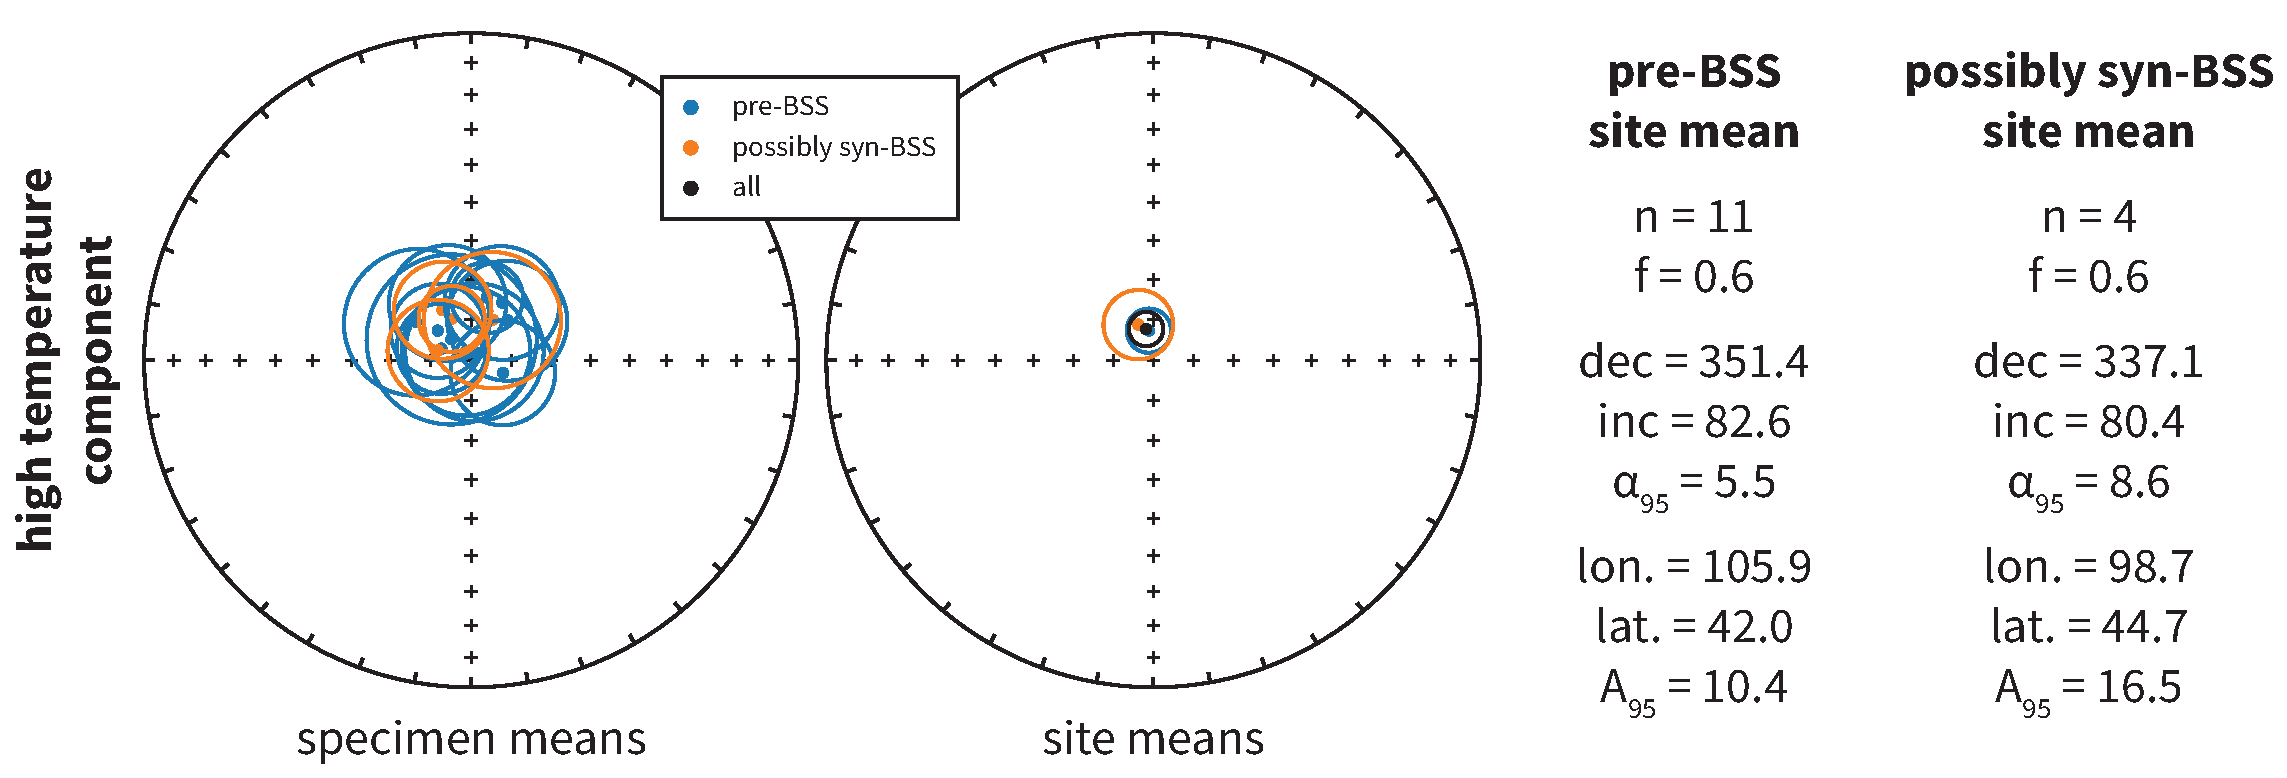
\includegraphics[width=\textwidth]{figures/Xiajiang/lower-upper-comparison.pdf}
    \caption[Comparison of the high temperature component from sites that are pre-Bitter Springs Stage and sites that could be syn-Bitter Springs Stage.]{Comparison of the high temperature component from sites that are unambiguously constrained by the geochronology to be pre-Bitter Springs Stage and sites that could be syn-Bitter Springs Stage (Fig. \ref{fig:stratigraphic-sections}). The angular difference between the two site mean directions is 3.0\degrees.}
    \label{fig:lower-upper-comparison}
\end{figure}

We compare the high temperature components obtained from the 11 sites that are unambiguously pre-Bitter Springs Stage, with the high temperature components obtained from the four sites that could be syn-Bitter Springs Stage. After converting all sites into a single polarity and applying a tilt and inclination correction, the two site mean directions have an angular difference of 3.0\degrees, and a common mean test cannot reject the null hypothesis at the 95\% confidence level that the specimen mean directions were drawn from distributions that share a common mean direction (in the Watson V test, $V$ = 0.8 and $V_{crit}$ = 6.9; Fig. \ref{fig:lower-upper-comparison}). This angular difference is much less than would be expected for Bitter Springs Stage TPW, indicating that the Nanhua Basin was in a similar position throughout Xiajiang Group deposition and that the sites can be grouped into a single paleomagnetic pole. However, ambiguity surrounding the age of the 4 sites that could be syn-Bitter Springs Stage hinders the ability to draw firm conclusions regarding TPW using the Xiajiang Group data alone. To gain more robust insight, we can assess the Xiajiang Group data in the context of the other Tonian South China poles.

The new 813$\pm$3~Ma Xiajiang Group pole and the new 804.9$\pm$0.4~Ma date on the Madiyi Formation pole provide paleomagnetic constraints on the position of South China before and during the Bitter Springs Stage. Additionally, the 821.6$\pm$0.2~Ma date on the Xiaofeng dikes pole constrains it to be pre-Bitter Springs Stage (although prior interpretations have taken the Xiaofeng dikes pole to represent a syn-Bitter Springs Stage position of South China using its previously assigned age of 802$\pm$10~Ma; \citealp{Maloof2006a, Jing2019a}). The pre-Bitter Springs Stage Xiaofeng dikes pole and the syn-Bitter Springs Stage Madiyi Formation pole share a common mean (Fig. \ref{fig:SChina-APWP}). Interpreting these two poles alone would suggest that South China was in a stable position between ca. 821 and 805~Ma in contrast to the prediction of the TPW hypothesis.

\begin{figure}[h!]
    \centering
    \includegraphics[width=\textwidth]{figures/Xiajiang/TPW-MC.pdf}
    \caption[Results of Monte Carlo analysis of hypothesized ca. 810~Ma rapid true polar wander motion.]{Results of Monte Carlo analysis of hypothesized ca. 810~Ma rapid true polar wander motion. \textbf{A)} Virtual geomagnetic poles (VGPs) for the Xiajiang Group, Madiyi Formation, and Lower and Upper Grusdievbreen Formation paleomagnetic poles randomly sampled from Fisherian distributions ($n=10,000$). South China is shown in its present day location, and Svalbard is rotated such that the 4 poles lie along a great circle. \textbf{B)} Ages of the Xiajiang Group and Madiyi Formation poles randomly sampled from uniform and Gaussian distributions respectively. \textbf{C)} Angular difference between randomly selected VGP pairs in A. \textbf{D)} Plate velocity of South China implied by A and B, and the plate velocity of Svalbard implied by A and assuming that the Upper Grusdievbreen Formation pole is 1--10~m.y. younger than the Lower Grusdievbreen Formation pole. The dashed vertical line is the $\sim$20~cm/yr plate velocity limit suggested by \citet{Conrad2001a} and \citet{Zahirovic2015a}.}
    \label{fig:TPW-MC}
\end{figure}

\begin{figure}[!htbp]
    \centering
    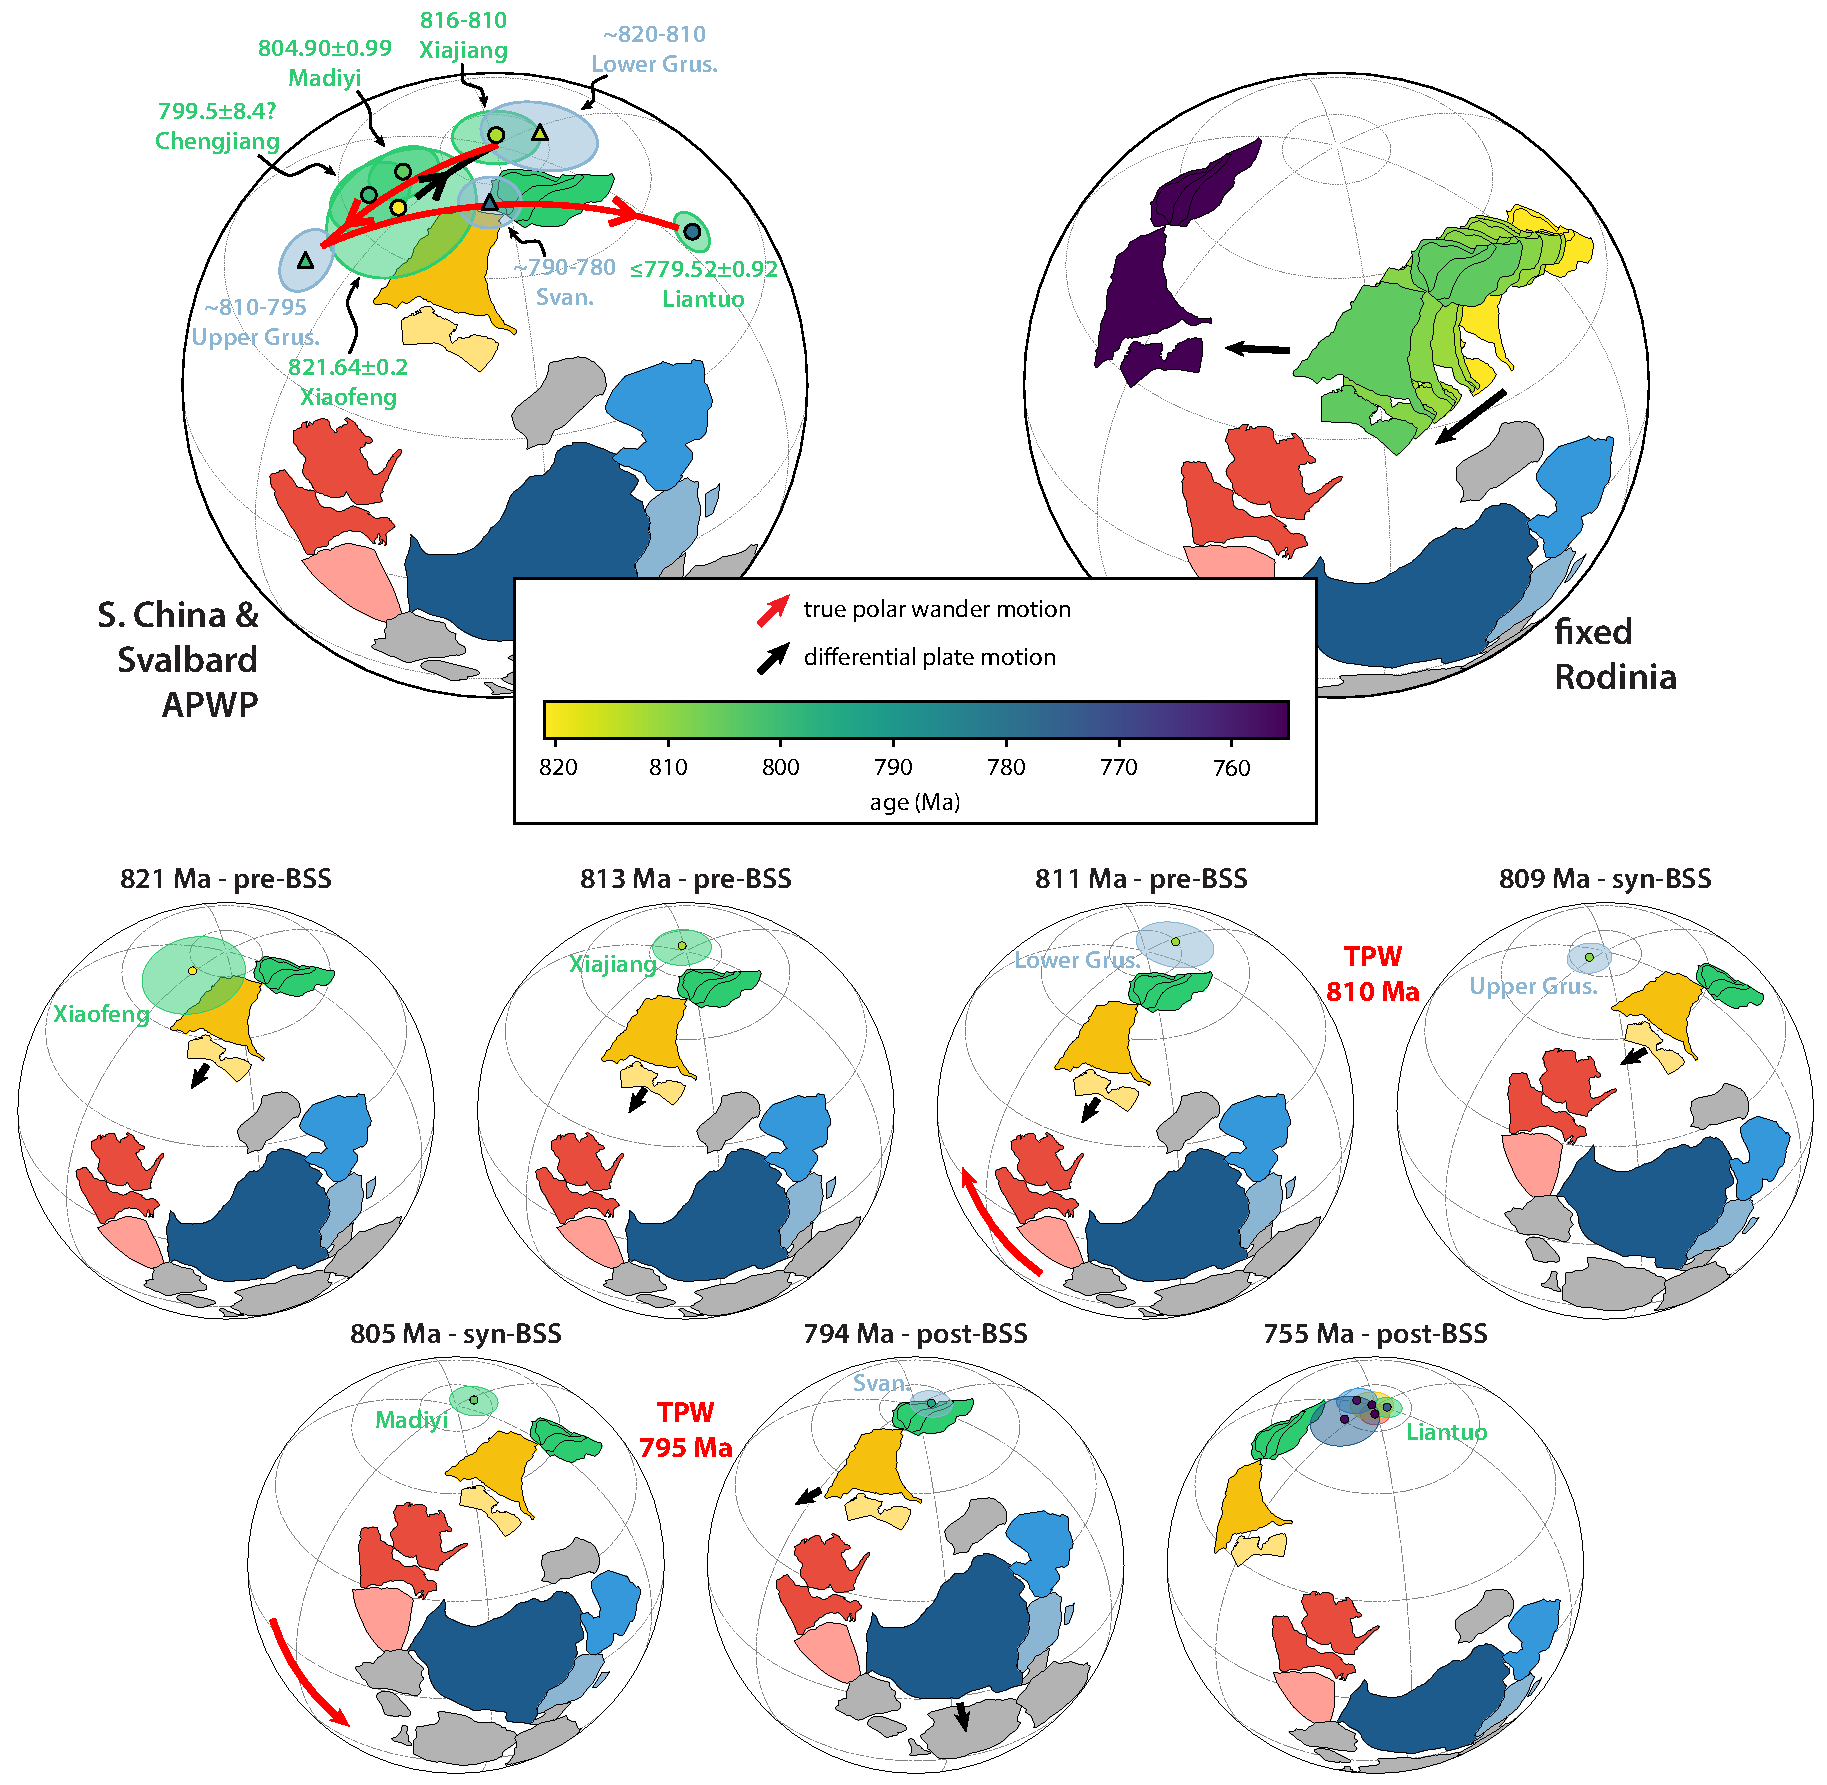
\includegraphics[width=\textwidth]{figures/Xiajiang/BSS-APWP.pdf}
    \caption[Continuous paleogeographic model if Tonian paleomagnetic poles from South China are interpreted as recording differential plate motion superimposed upon Bitter Springs Stage true polar wander.]{Continuous paleogeographic model if Tonian paleomagnetic poles from South China are interpreted as recording differential plate motion superimposed upon Bitter Springs Stage (BSS) true polar wander (TPW). In the upper left, the tectonic blocks are shown in a ca. 813~Ma reconstruction, and the apparent polar wander paths (APWPs) of South China and Svalbard are aligned along two great circles. In the upper right, Rodinia (Laurentia + associated cratons) is fixed in a ca. 755~Ma reconstruction to show the differential motion of South China-India-Rayner relative to Rodinia. The seven lower reconstructions show pre-, syn-, and post-BSS reconstructions in a celestial reference frame. Note that differential plate motion of South China-India-Rayner continues through ca. 810~Ma rapid TPW defined by the Lower and Upper Grusdievbreen Formation poles of Svalbard. Euler rotations for this paleogeographic model are shown in Table S9.}
    \label{fig:BSS-APWP}
\end{figure}

However, the pre-Bitter Springs Stage Xiajiang Group pole has a distinct position from the syn-Bitter Springs Stage Madiyi Formation pole, with an angular difference of 19\degrees between the means of the poles (Fig. \ref{fig:SChina-APWP}). In order to assess this angular difference in comparison to the poles from Svalbard while accounting for the uncertainty on the pole positions and ages, we take a Monte Carlo approach in which 10,000 random draws are taken from Fisherian distributions for the pole positions and from Gaussian distributions for the pole ages (Figs. \ref{fig:TPW-MC}A and \ref{fig:TPW-MC}B; \citealp{Swanson-Hysell2014b}). Taking this approach, the angular difference between the Xiajiang Group and Madiyi Formation poles is 11--27\degrees at the 95\% confidence level, whereas the angular difference between the Lower and Upper Grusdievbreen Formation poles is much higher at 41--62\degrees at the 95\% confidence level (Fig. \ref{fig:TPW-MC}C). In fact, the probability that a Xiajiang Group--Madiyi Formation pole pair has an equal or larger angular difference than a Lower--Upper Grusdievbreen Formation pole pair is only 8.5$\times$10$^{-5}$\% (calculated using the means and standard deviations of the normal distributions in Fig. \ref{fig:TPW-MC}C). As such, the angular difference between the pre- and syn-Bitter Springs Stage poles is significantly less than predicted by the hypothesis that the Svalbard paleomagnetic poles are primary and that their differing positions is the result of TPW. Therefore, this Monte Carlo analysis suggests that the angular difference between the pole pairs from South China and Svalbard can not be straight-forwardly interpreted to be associated with a single TPW rotation.

The velocity of South China implied by the Xiajiang Group and Madiyi Formation poles is also slower than that implied for Svalbard by the Lower and Upper Grusdievbreen Formation poles, being 14--48~cm/yr rather than 60--284~cm/yr at the 95\% confidence level, if the Upper Grusdievbreen Formation pole is taken to be 1 to 10~m.y. younger than the Lower Grusdievbreen Formation pole (\citealp{Maloof2006a}; Fig. \ref{fig:TPW-MC}D). In contrast to the very rapid rates implied by the Svalbard poles, the rate for South China's motion is at the upper end of the range of velocities suggested by plate kinematic reconstructions (Fig. \ref{fig:TPW-MC}D; \citealp{Meert1993a, Zahirovic2015a}).

However, the smaller angular difference between the Xiajiang Group and Madiyi Formation poles relative to the Lower and Upper Grusdievbreen Formation poles could be reconciled with the TPW hypothesis if differential plate motion between South China and Svalbard is superimposed on TPW motion between ca. 813 and 805~Ma \citep{Evans2003a}. For example, if rapid TPW occurred ca. 810~Ma, the Xiajiang Group and Madiyi Formation poles should lie along the great circle between the Lower and Upper Grusdievbreen Formation poles, implying a unique reconstruction for South China relative to Svalbard (Fig. \ref{fig:BSS-APWP}). This configuration also aligns the great circle between the syn-Bitter Springs Stage Upper Grusdievbreen Formation and post-Bitter Springs Stage Svanbergfjellet Formation Svalbard poles with that of the syn-Bitter Springs Stage Madiyi Formation and post-Bitter Springs Stage Liantuo Formation South China poles (Fig. \ref{fig:BSS-APWP}). In the TPW hypothesis, this second great circle would represent the second rapid TPW event ca. 795~Ma. However, South China could have continued to move via differential plate tectonics along the trajectory implied by the difference between the ca. 821~Ma Xiaofeng dikes and the ca. 813~Ma Xiajiang Formation poles through ca. 810~Ma TPW rotation (Fig. \ref{fig:BSS-APWP}). In such a scenario, the differential plate tectonic motion of South China is approximately opposite the trajectory of the hypothesized TPW rotation (Fig. \ref{fig:BSS-APWP}), which would be observed in the paleomagnetic record as a smaller angular difference between pre- to syn-Bitter Springs Stage paleomagnetic poles from South China than what would be predicted for TPW alone. Put another way, differential plate tectonic motion could have driven South China in the opposite direction of TPW motion, causing South China to move a smaller distance in a celestial reference frame relative to other tectonic blocks that were not experiencing such differential plate tectonic motion between ca. 813 and 805~Ma, such as Svalbard.

Importantly, if rapid TPW did occur ca. 810~Ma, and differential plate motion between South China and Svalbard ca. 813--805~Ma is superimposed upon that TPW motion to explain the smaller angular difference between the Xiajiang Group and Madiyi Formation poles relative to the Lower and Upper Grusdievbreen Formation poles, then it is required that South China was separate from Rodinia (i.e. the Separate model in Figure \ref{fig:Rodinia-models}). It is well established that Svalbard was connected to Laurentia via Greenland until Silurian-Devonian translation along Greenland's margin and subsequent rifting away from Greenland in the Eocene \citep{Torsvik2016a}. Therefore, if South China was moving differentially relative to Svalbard ca. 813--805~Ma, South China must have been moving differentially relative to Rodinia, and therefore must have been separate from Rodinia. Furthermore, the alignment of paleomagnetic poles from South China and Svalbard along great circles places South China at high latitudes, with the long southeastern margin of the Cathaysia block facing Svalbard (Fig. \ref{fig:BSS-APWP}). However, ca. 755~Ma paleomagnetic poles require that a Periphery model has South China-India-Rayner connected to Rodinia in a different orientation via northwestern Australia (Fig. \ref{fig:Rodinia-models}). Even if the Lower Grusdievbreen Formation pole is interpreted as a Paleozoic overprint \citep{Michalski2011a}, if the syn-Bitter Springs Stage Upper Grusdievbreen Formation and post-Bitter Springs Stage Svanbergfjellet Formation Svalbard poles are primary, rapid TPW could be interpreted to have occurred ca. 795~Ma. In this scenario, South China is still required to be separate from Rodinia in order to align the great circle between path with that of the syn-Bitter Springs Stage Madiyi Formation and post-Bitter Springs Stage Liantuo Formation South China poles (Fig. \ref{fig:BSS-APWP}).

Regardless of whether the ca. 821~Ma to ca. 805~Ma poles are interpreted as recording TPW counteracted by plate tectonic motion or a relatively stable position of South China (as in Figure \ref{fig:SChina-APWP}F), South China is peripheral or disconnected from Rodinia.

\section{Conclusions}

The geochronologic and paleomagnetic data developed from the Xiajiang Group constrain the amalgamation of the Yangtze and Cathaysia blocks of South China to have completed between ca. 830~Ma and 815.73$\pm$0.18~Ma at high latitudes. A consistent high latitude position is implied by poles from ca. 821~Ma to 805~Ma with a continued high latitude position ca. 780~Ma following South China transiting over the pole. These paleolatitudes, as well as convergent orogenesis between the Yangtze and Cathaysia blocks and continued arc activity along the northwest margin of the South China craton during the Tonian and into the Cryogenian, cannot be reconciled with the Missing Link model that places South China in the core of a stable Rodinia continent. The angular difference in pole position between the ca. 813~Ma (pre-Bitter Springs Stage) Xiajiang Group pole and ca. 805~Ma (syn-Bitter Springs Stage) Madiyi Formation pole is significantly less than that predicted for the Bitter Springs Stage TPW hypothesis. The poles could be interpreted to indicate a relatively stable high latitude position for South China inconsistent with TPW. However, it is possible to interpret the poles as TPW rotation counteracted by plate tectonic motion. In this scenario, South China must be considered to be distinct from Rodinia. Whether or not the paleomagnetic poles are interpreted as recording TPW, they constrain South China to either have been connected to Rodinia along its periphery, or disconnected from the (super)continent entirely.

\section{Acknowledgements}

Research was supported by National Science Foundation grants EAR-1547434 and EAR-1547537 to N.L.S-.H. and F.A.M. CUGB research was supported by National Natural Science Foundation of China grant 41830215 to S.H.Z. Maoyan Zhu supported research logistics in the field. Oliver Abbitt prepared specimens for paleomagnetic analyses.


%%%%%%%%%%%%%%%%%%%%%%%%
%%%%% BIBLIOGRAPHY %%%%%
%%%%%%%%%%%%%%%%%%%%%%%%

\bibliography{references}

%%%%%%%%%%%%%%%%%%%%
%%%%% APPENDIX %%%%%
%%%%%%%%%%%%%%%%%%%%

\appendix
\include{SI-SEAIs}
\include{SI-Tambien}
\chapter[Supporting Information for ``Tonian paleomagnetism from South China permits an inclusive Rodinia or Bitter Springs Stage true polar wander, but not both''][Supporting Information - Xiajiang Group]{Supporting Information for ``Tonian paleomagnetism from South China permits an inclusive Rodinia or Bitter Springs Stage true polar wander, but not both''}

\begin{figure}[h!]
    \centering
    \includegraphics[width=0.8\textwidth]{figures/Xiajiang/bootstrap-CDF.pdf}
    \caption[Results of the bootstrap fold test for the Xiajiang Group high-temperature component.]{Results of the bootstrap fold test \citep{Tauxe1994a} for the Xiajiang Group high-temperature component. The tightest grouping of site mean directions is obtained between 68 and 103\% unfolding at the 95\% confidence level. Since this range encompasses 100\%, the high-temperature component passes the fold test, constraining the high-temperature component to have been acquired prior to Mesozoic folding of the Xiajiang Group \citep{Li2016c, Ma2019a}.}
    \label{fig:bootstrap-CDF}
\end{figure}

\begin{figure}[h!]
    \centering
    \includegraphics[width=0.9\textwidth]{figures/Xiajiang/tuff-photos.jpg}
    \caption[Photographs of tuffs in the Xiajiang Group.]{Photographs of tuffs that yielded consistent and concordant CA-ID-TIMS $^{206}$Pb/$^{238}$U zircon dates. Red arrows point to the sampled tuffs. \textbf{A)} H2-470. \textbf{B)} H3-60. \textbf{C)} H3-8. \textbf{D)} QR-74. \textbf{E)} L4-2. No photograph is available for sample L1-27.}
    \label{fig:tuff-photos}
\end{figure}

\begin{figure}[h!]
    \centering
    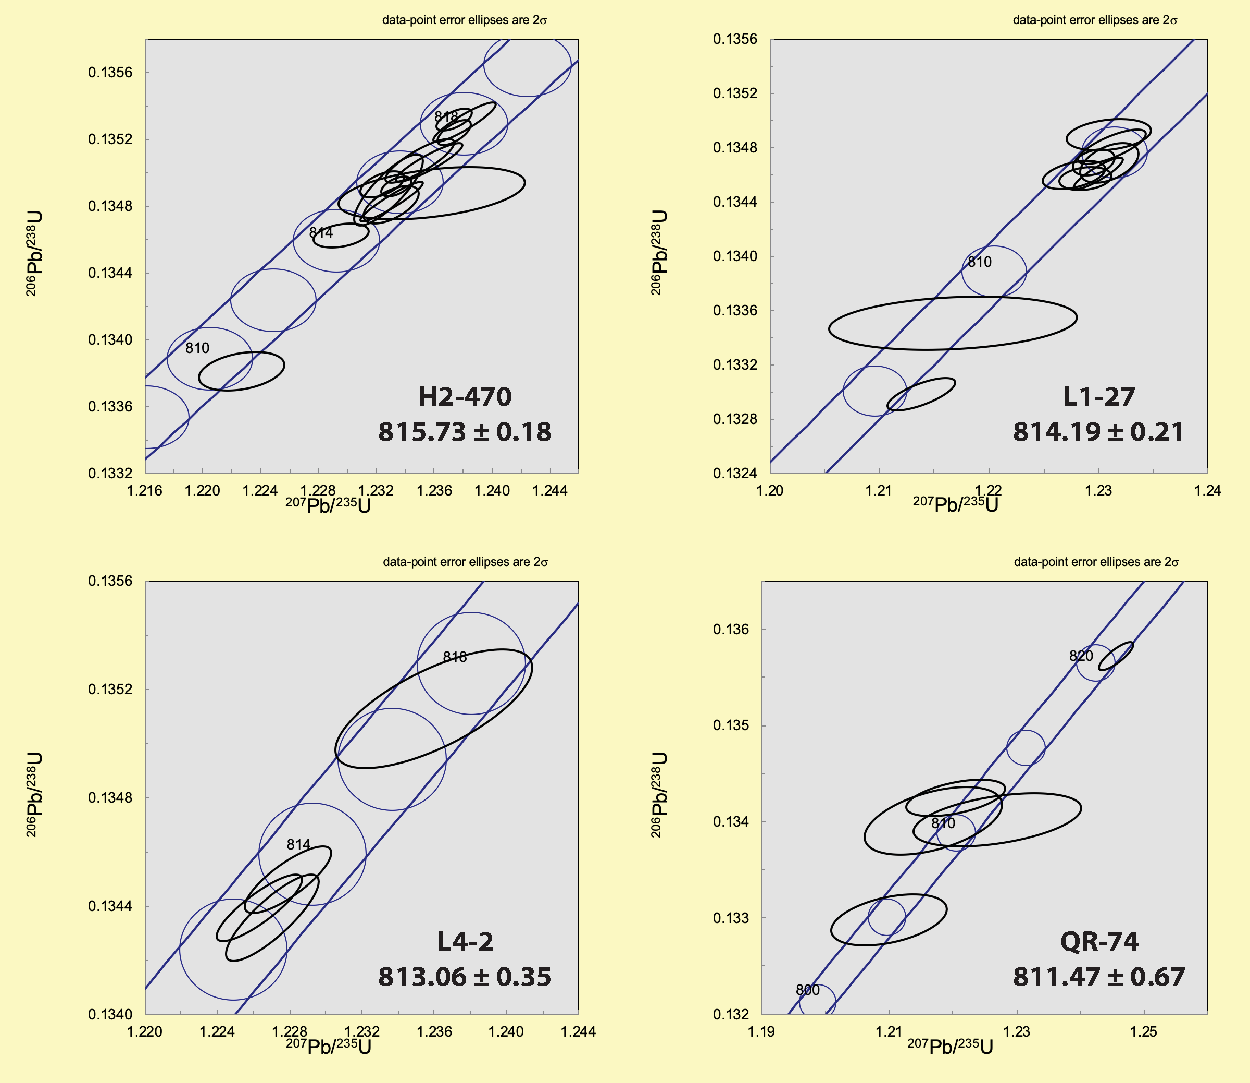
\includegraphics[width=0.9\textwidth]{figures/Xiajiang/concordia-1.pdf}
    \caption[Concordia diagrams for zircons from tuffs of the Xiajiang Group.]{Concordia diagrams for zircons from tuffs of the Xiajiang Group analyzed in this study. Individual zircon data are tabulated in Table SX.}
    \label{fig:concordia-1}
\end{figure}

\begin{figure}[h!]
    \centering
    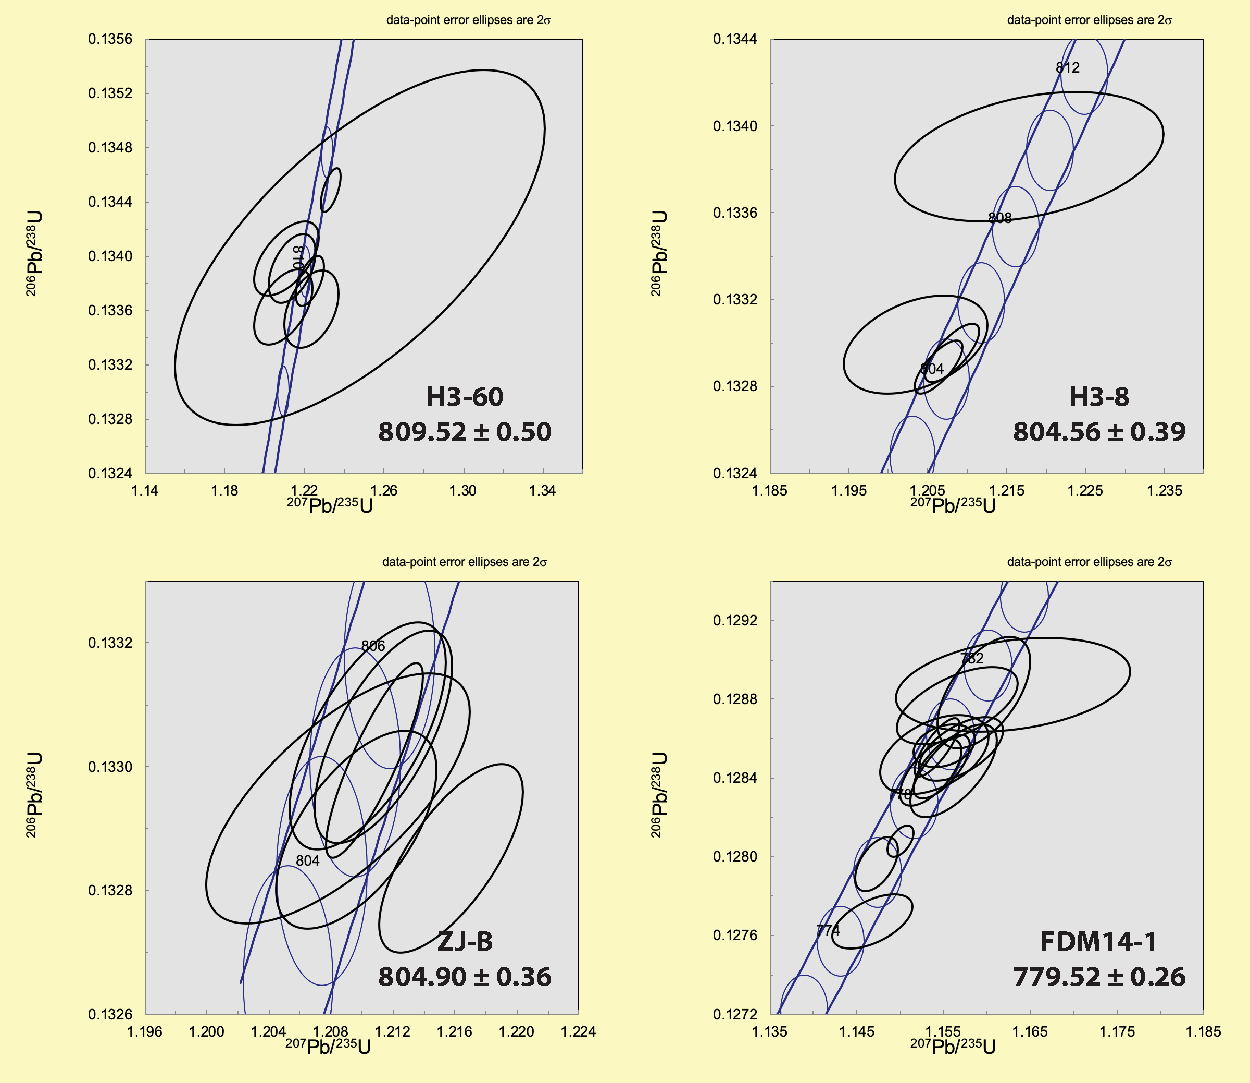
\includegraphics[width=0.9\textwidth]{figures/Xiajiang/concordia-2.pdf}
    \caption[Concordia diagrams for zircons from tuffs of the Xiajiang Group, Madiyi Formation, and Liantuo Formation.]{Concordia diagrams for zircons from tuffs of the Xiajiang Group (H3-60 and H3-8), Madiyi Formation (ZJ-B), and Liantuo Formation (FDM14-1) analyzed in this study. Individual zircon data are tabulated in Table SX.}
    \label{fig:concordia-2}
\end{figure}

\begin{figure}[h!]
    \centering
    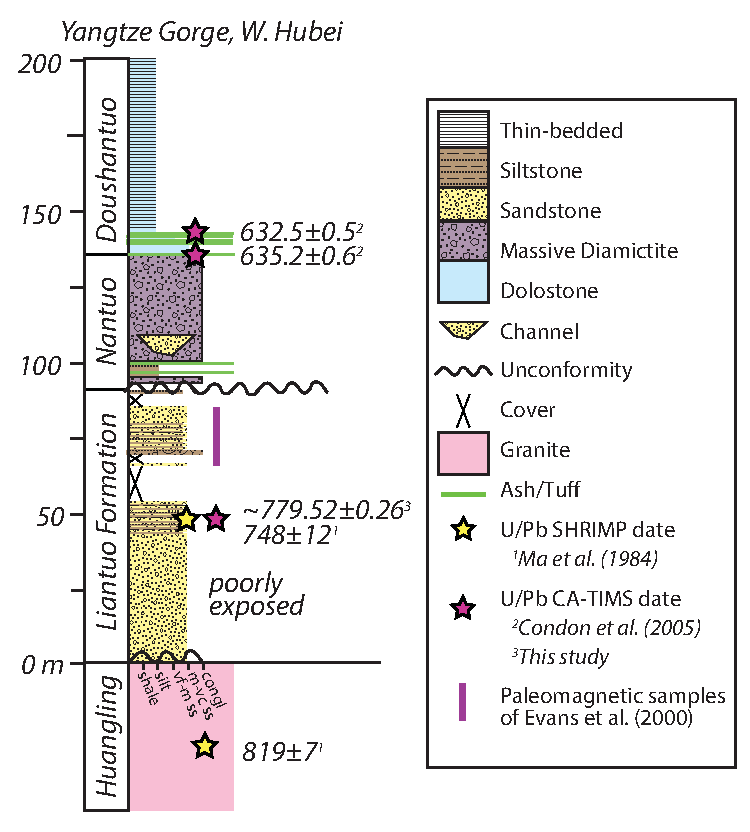
\includegraphics[width=0.8\textwidth]{figures/Xiajiang/FDM14-1-strat.pdf}
    \caption[Tonian-Cryogenian stratigraphy of the Yangtze Gorge.]{Tonian-Cryogenian stratigraphy of the Yangtze Gorge, from where the paleomagnetic and geochronologic data for the Liantuo Formation are developed.}
    \label{fig:FDM14-1-strat}
\end{figure}

\begin{sidewaystable*}[h!]
\tiny
\vspace*{1 cm}
\caption{U-Pb data for analyzed zircons from H2-470.}
\vspace{1 cm}
\setlength\tabcolsep{3.5pt}
\begin{tabular}{cccccccccccccccccccc}
& \multicolumn{8}{l}{Dates (Ma)} & \multicolumn{4}{l}{Composition} & \multicolumn{7}{l}{Isotopic Ratios} \\
\cline{2-20}\\
& $^a$ & & $^b$ & & $^{a,b}$ & & & $^c$ & $^d$ & $^e$ & $^f$ & $^{g}$ & $^h$ & $^{a,i}$ & & $^{b,i}$ & & $^{a,b,i}$ & \\	
& \underline{$^{206}$Pb} & $\pm$ & \underline{$^{207}$Pb} & $\pm$ & \underline{$^{207}$Pb} & $\pm$ & corr. & & \underline{Th} & Pb\** & Pb$_c$ & \underline{Pb\**} & \underline{$^{206}$Pb} & \underline{$^{206}$Pb} & $\pm$ & \underline{$^{207}$Pb} & $\pm$ & \underline{$^{207}$Pb} & $\pm$ \\		
fraction & $^{238}$U & (2$\sigma$) & $^{235}$U & (2$\sigma$) & $^{206}$Pb & (2$\sigma$) & coef. & \% disc. & U & (pg) & (pg) & Pb$_c$ & $^{204}$Pb & $^{238}$Pb & (2$\sigma\%$) & $^{235}$U & (2$\sigma\%$) & $^{206}$Pb & (2$\sigma\%$) \\
\hline \\
z9  & 809.55 & 0.53 & 811.00 & 1.10 & 814.95 & 3.88 & 0.33 & 0.69  & 0.90 & 15.6  & 0.25 & 62.2   & 3392  & 0.133808 & 0.070220 & 1.222669 & 0.196189 & 0.066301 & 0.182537 \\
z11 & 814.18 & 0.34 & 814.14 & 0.70 & 814.03 & 2.46 & 0.34 & 0.01  & 0.74 & 24.5  & 0.17 & 141.8  & 7993  & 0.134622 & 0.044107 & 1.229565 & 0.125086 & 0.066272 & 0.113043 \\
\rowcolor{Yellow}
z14 & 815.23 & 0.52 & 815.70 & 0.71 & 816.99 & 2.14 & 0.59 & 0.25  & 0.77 & 151.5 & 0.32 & 479.9  & 26838 & 0.134807 & 0.067705 & 1.232995 & 0.126378 & 0.066366 & 0.096844 \\
\rowcolor{Yellow}
z2  & 815.35 & 0.54 & 815.71 & 0.80 & 816.70 & 1.69 & 0.93 & 0.20  & 0.58 & 181.3 & 0.18 & 1013.2 & 59304 & 0.134828 & 0.070797 & 1.233019 & 0.143199 & 0.066356 & 0.074214 \\
\rowcolor{Yellow}
z3  & 815.62 & 0.72 & 816.98 & 2.39 & 820.70 & 8.28 & 0.41 & 0.65  & 0.62 & 95.6  & 5.15 & 18.6   & 1093  & 0.134876 & 0.093966 & 1.235816 & 0.424989 & 0.066484 & 0.394981 \\
\rowcolor{Yellow}
z7  & 815.73 & 0.99 & 815.63 & 0.88 & 815.35 & 1.90 & 0.82 & -0.02 & 0.88 & 38.7  & 0.30 & 128.9  & 7036  & 0.134895 & 0.128998 & 1.232832 & 0.157563 & 0.066314 & 0.084703 \\
\rowcolor{Yellow}
z8  & 815.85 & 0.27 & 815.87 & 0.40 & 815.92 & 1.25 & 0.53 & 0.04  & 0.72 & 35.1  & 0.15 & 226.9  & 12842 & 0.134917 & 0.035031 & 1.233366 & 0.070632 & 0.066332 & 0.050324 \\
\rowcolor{Yellow}
z12 & 815.93 & 0.36 & 815.43 & 0.56 & 814.06 & 1.78 & 0.54 & -0.20 & 0.78 & 23.6  & 0.16 & 148.4  & 8295  & 0.134931 & 0.047158 & 1.232398 & 0.100758 & 0.066273 & 0.078418 \\
z1  & 816.69 & 0.53 & 816.90 & 0.84 & 817.48 & 1.95 & 0.90 & 0.13  & 0.76 & 132.2 & 0.74 & 179.4  & 10069 & 0.135064 & 0.069554 & 1.235639 & 0.150465 & 0.066381 & 0.087256 \\
z4  & 816.73 & 0.61 & 816.60 & 0.88 & 816.24 & 2.11 & 0.83 & -0.03 & 0.73 & 32.6  & 0.12 & 272.7  & 15417 & 0.135072 & 0.079228 & 1.234975 & 0.156380 & 0.066342 & 0.095355 \\
z6  & 817.69 & 0.34 & 817.70 & 0.42 & 817.73 & 1.19 & 0.65 & 0.04  & 0.86 & 60.2  & 0.26 & 232.1  & 12723 & 0.135239 & 0.044110 & 1.237385 & 0.074873 & 0.066389 & 0.046714 \\
z5  & 818.04 & 0.54 & 818.01 & 0.80 & 817.92 & 1.78 & 0.90 & 0.02  & 0.72 & 57.6  & 0.14 & 408.6  & 23141 & 0.135301 & 0.070555 & 1.238068 & 0.143195 & 0.066395 & 0.078665 \\
z10 & 818.13 & 0.30 & 817.69 & 0.44 & 816.47 & 1.32 & 0.62 & -0.17 & 0.76 & 50.0  & 0.16 & 311.7  & 17475 & 0.135318 & 0.038917 & 1.237363 & 0.079176 & 0.066349 & 0.053969 \\
z16 & 826.68 & 0.32 & 824.61 & 0.43 & 819.04 & 1.27 & 0.61 & -0.90 & 0.74 & 93.5  & 0.30 & 311.7  & 17581 & 0.136824 & 0.040989 & 1.252669 & 0.076810 & 0.066431 & 0.051484 \\
z13 & 830.20 & 0.53 & 825.34 & 0.85 & 812.27 & 2.03 & 0.87 & -2.17 & 0.75 & 62.5  & 0.38 & 164.3  & 9250  & 0.137445 & 0.068375 & 1.254296 & 0.149999 & 0.066216 & 0.091207 \\
z15 & 844.63 & 0.31 & 837.47 & 0.90 & 818.55 & 3.17 & 0.28 & -3.16 & 1.03 & 41.3  & 0.76 & 54.4   & 2879  & 0.139994 & 0.038917 & 1.281393 & 0.158093 & 0.066415 & 0.148349 \\
\end{tabular}

\flushleft \emph{Notes:} \\
Colored rows indicate fractions included in the calculation of the reported sample age. \\
Isotopic dates calculated using $\lambda$238 = 1.55125$\times$10$^{-10}$ and $\lambda$235 = 9.8485$\times$10$^{-10}$ \citep{Jaffey1971a}. \\
 $^{a}$  Corrected for initial Th/U disequilibrium using radiogenic $^{208}$Pb and Th/U[magma] = 2.8. \\
 $^{b}$ Corrected for initial Pa/U disequilibrium using initial fraction activity ratio [$^{231}$Pa]/[$^{235}$U] = 1.10000. \\
 $^{c}$ \% discordance = 100 - (100 $\times$ ($^{206}$Pb/$^{238}$U date) / ($^{207}$Pb/$^{206}$Pb date)) \\
 $^{d}$ Th contents calculated from radiogenic $^{208}$Pb and $^{230}$Th-corrected $^{206}$Pb/$^{238}$U date of the sample, assuming concordance between U-Pb Th-Pb systems. \\
 $^{e}$ Total mass of radiogenic Pb. \\
 $^{f}$ Total mass of common Pb. \\
 $^{g}$ Ratio of radiogenic Pb (including $^{208}$Pb) to common Pb. \\
 $^{h}$ Measured ratio corrected for fractionation and spike contribution only. \\
 $^{i}$ Measured ratios corrected for fractionation, tracer and blank.
\end{sidewaystable*}

\begin{sidewaystable*}[h!]
\tiny
\vspace*{1 cm}
\caption{U-Pb data for analyzed zircons from L1-27.}
\vspace{1 cm}
\setlength\tabcolsep{3.5pt}
\begin{tabular}{cccccccccccccccccccc}
& \multicolumn{8}{l}{Dates (Ma)} & \multicolumn{4}{l}{Composition} & \multicolumn{7}{l}{Isotopic Ratios} \\
\cline{2-20}\\
& $^a$ & & $^b$ & & $^{a,b}$ & & & $^c$ & $^d$ & $^e$ & $^f$ & $^{g}$ & $^h$ & $^{a,i}$ & & $^{b,i}$ & & $^{a,b,i}$ & \\	
& \underline{$^{206}$Pb} & $\pm$ & \underline{$^{207}$Pb} & $\pm$ & \underline{$^{207}$Pb} & $\pm$ & corr. & & \underline{Th} & Pb\** & Pb$_c$ & \underline{Pb\**} & \underline{$^{206}$Pb} & \underline{$^{206}$Pb} & $\pm$ & \underline{$^{207}$Pb} & $\pm$ & \underline{$^{207}$Pb} & $\pm$ \\		
fraction & $^{238}$U & (2$\sigma$) & $^{235}$U & (2$\sigma$) & $^{206}$Pb & (2$\sigma$) & coef. & \% disc. & U & (pg) & (pg) & Pb$_c$ & $^{204}$Pb & $^{238}$Pb & (2$\sigma\%$) & $^{235}$U & (2$\sigma\%$) & $^{206}$Pb & (2$\sigma\%$) \\
\hline \\
z5  & 804.84 & 0.56 & 806.95 & 1.16 & 812.78 & 3.42  & 0.72 & 1.01  & 0.73 & 50.5 & 0.82 & 61.7  & 3500 & 0.132980 & 0.073384 & 1.213839 & 0.207803 & 0.066232 & 0.160083 \\
z6  & 807.82 & 0.91 & 808.27 & 4.24 & 809.52 & 15.58 & 0.22 & 0.24  & 0.79 & 7.0  & 0.63 & 11.1  & 638  & 0.133504 & 0.119942 & 1.216721 & 0.761579 & 0.066129 & 0.744112 \\
\rowcolor{Yellow}
z9  & 813.90 & 0.39 & 813.80 & 0.88 & 813.52 & 3.20  & 0.22 & -0.02 & 0.85 & 27.2 & 0.32 & 85.4  & 4697 & 0.134572 & 0.050696 & 1.228808 & 0.156387 & 0.066256 & 0.149699 \\
\rowcolor{Yellow}
z8  & 814.06 & 0.48 & 813.32 & 1.08 & 811.29 & 3.66  & 0.43 & -0.31 & 0.98 & 16.3 & 0.31 & 52.0  & 2787 & 0.134600 & 0.062729 & 1.227755 & 0.192831 & 0.066185 & 0.172067 \\
\rowcolor{Yellow}
z2  & 814.11 & 0.53 & 814.33 & 0.83 & 814.92 & 1.97  & 0.88 & 0.13  & 0.62 & 55.9 & 0.33 & 169.6 & 9852 & 0.134610 & 0.068803 & 1.229970 & 0.148922 & 0.066300 & 0.088455 \\
\rowcolor{Yellow}
z12 & 814.55 & 0.67 & 814.81 & 0.99 & 815.50 & 3.29  & 0.46 & 0.14  & 1.10 & 18.0 & 0.26 & 68.8  & 3583 & 0.134688 & 0.087437 & 1.231029 & 0.177274 & 0.066318 & 0.153859 \\
\rowcolor{Yellow}
z11 & 814.57 & 0.44 & 814.14 & 0.70 & 812.95 & 2.47  & 0.35 & -0.17 & 0.87 & 19.5 & 0.23 & 86.0  & 4714 & 0.134691 & 0.058009 & 1.229554 & 0.125152 & 0.066238 & 0.113683 \\
z4  & 815.24 & 0.59 & 814.91 & 1.15 & 814.02 & 3.28  & 0.75 & -0.12 & 0.84 & 18.9 & 0.27 & 71.1  & 3926 & 0.134808 & 0.076864 & 1.231253 & 0.205803 & 0.066271 & 0.153331 \\
z7  & 815.75 & 0.53 & 814.78 & 1.43 & 812.13 & 5.12  & 0.27 & -0.41 & 0.88 & 9.1  & 0.27 & 33.0  & 1818 & 0.134898 & 0.069355 & 1.230966 & 0.254447 & 0.066212 & 0.242857 \\
\end{tabular}

\flushleft \emph{Notes:} \\
Colored rows indicate fractions included in the calculation of the reported sample age. \\
Isotopic dates calculated using $\lambda$238 = 1.55125$\times$10$^{-10}$ and $\lambda$235 = 9.8485$\times$10$^{-10}$ \citep{Jaffey1971a}. \\
 $^{a}$  Corrected for initial Th/U disequilibrium using radiogenic $^{208}$Pb and Th/U[magma] = 2.8. \\
 $^{b}$ Corrected for initial Pa/U disequilibrium using initial fraction activity ratio [$^{231}$Pa]/[$^{235}$U] = 1.10000. \\
 $^{c}$ \% discordance = 100 - (100 $\times$ ($^{206}$Pb/$^{238}$U date) / ($^{207}$Pb/$^{206}$Pb date)) \\
 $^{d}$ Th contents calculated from radiogenic $^{208}$Pb and $^{230}$Th-corrected $^{206}$Pb/$^{238}$U date of the sample, assuming concordance between U-Pb Th-Pb systems. \\
 $^{e}$ Total mass of radiogenic Pb. \\
 $^{f}$ Total mass of common Pb. \\
 $^{g}$ Ratio of radiogenic Pb (including $^{208}$Pb) to common Pb. \\
 $^{h}$ Measured ratio corrected for fractionation and spike contribution only. \\
 $^{i}$ Measured ratios corrected for fractionation, tracer and blank.
\end{sidewaystable*}

\begin{sidewaystable*}[h!]
\tiny
\vspace*{1 cm}
\caption{U-Pb data for analyzed zircons from L4-2.}
\vspace{1 cm}
\setlength\tabcolsep{3.5pt}
\begin{tabular}{cccccccccccccccccccc}
& \multicolumn{8}{l}{Dates (Ma)} & \multicolumn{4}{l}{Composition} & \multicolumn{7}{l}{Isotopic Ratios} \\
\cline{2-20}\\
& $^a$ & & $^b$ & & $^{a,b}$ & & & $^c$ & $^d$ & $^e$ & $^f$ & $^{g}$ & $^h$ & $^{a,i}$ & & $^{b,i}$ & & $^{a,b,i}$ & \\	
& \underline{$^{206}$Pb} & $\pm$ & \underline{$^{207}$Pb} & $\pm$ & \underline{$^{207}$Pb} & $\pm$ & corr. & & \underline{Th} & Pb\** & Pb$_c$ & \underline{Pb\**} & \underline{$^{206}$Pb} & \underline{$^{206}$Pb} & $\pm$ & \underline{$^{207}$Pb} & $\pm$ & \underline{$^{207}$Pb} & $\pm$ \\		
fraction & $^{238}$U & (2$\sigma$) & $^{235}$U & (2$\sigma$) & $^{206}$Pb & (2$\sigma$) & coef. & \% disc. & U & (pg) & (pg) & Pb$_c$ & $^{204}$Pb & $^{238}$Pb & (2$\sigma\%$) & $^{235}$U & (2$\sigma\%$) & $^{206}$Pb & (2$\sigma\%$) \\
\hline \\
\rowcolor{Yellow}
z5 & 812.67 & 0.73 & 812.99 & 0.96 & 813.86 & 2.20 & 0.84 & 0.18  & 0.64 & 28.3 & 0.17 & 170.0 & 9812 & 0.134357 & 0.096183 & 1.227035 & 0.171839 & 0.066266 & 0.100134 \\
\rowcolor{Yellow}
z3 & 812.88 & 0.57 & 812.67 & 0.88 & 812.09 & 2.13 & 0.85 & -0.07 & 0.76 & 96.5 & 0.70 & 137.1 & 7703 & 0.134393 & 0.074304 & 1.226330 & 0.157528 & 0.066210 & 0.096556 \\
\rowcolor{Yellow}
z1 & 813.47 & 0.57 & 813.40 & 0.89 & 813.19 & 2.27 & 0.81 & 0.00  & 0.79 & 72.4 & 0.46 & 157.4 & 8784 & 0.134497 & 0.074341 & 1.227932 & 0.159174 & 0.066245 & 0.103450 \\
z4 & 817.05 & 1.02 & 817.05 & 2.02 & 817.07 & 5.95 & 0.70 & 0.03  & 0.78 & 10.7 & 0.25 & 43.5  & 2442 & 0.135127 & 0.132953 & 1.235972 & 0.360619 & 0.066368 & 0.282745 \\
\end{tabular}

\flushleft \emph{Notes:} \\
Colored rows indicate fractions included in the calculation of the reported sample age. \\
Isotopic dates calculated using $\lambda$238 = 1.55125$\times$10$^{-10}$ and $\lambda$235 = 9.8485$\times$10$^{-10}$ \citep{Jaffey1971a}. \\
 $^{a}$  Corrected for initial Th/U disequilibrium using radiogenic $^{208}$Pb and Th/U[magma] = 2.8. \\
 $^{b}$ Corrected for initial Pa/U disequilibrium using initial fraction activity ratio [$^{231}$Pa]/[$^{235}$U] = 1.10000. \\
 $^{c}$ \% discordance = 100 - (100 $\times$ ($^{206}$Pb/$^{238}$U date) / ($^{207}$Pb/$^{206}$Pb date)) \\
 $^{d}$ Th contents calculated from radiogenic $^{208}$Pb and $^{230}$Th-corrected $^{206}$Pb/$^{238}$U date of the sample, assuming concordance between U-Pb Th-Pb systems. \\
 $^{e}$ Total mass of radiogenic Pb. \\
 $^{f}$ Total mass of common Pb. \\
 $^{g}$ Ratio of radiogenic Pb (including $^{208}$Pb) to common Pb. \\
 $^{h}$ Measured ratio corrected for fractionation and spike contribution only. \\
 $^{i}$ Measured ratios corrected for fractionation, tracer and blank.
\end{sidewaystable*}

\begin{sidewaystable*}[h!]
\tiny
\vspace*{1 cm}
\caption{U-Pb data for analyzed zircons from QR-74.}
\vspace{1 cm}
\setlength\tabcolsep{3.5pt}
\begin{tabular}{cccccccccccccccccccc}
& \multicolumn{8}{l}{Dates (Ma)} & \multicolumn{4}{l}{Composition} & \multicolumn{7}{l}{Isotopic Ratios} \\
\cline{2-20}\\
& $^a$ & & $^b$ & & $^{a,b}$ & & & $^c$ & $^d$ & $^e$ & $^f$ & $^{g}$ & $^h$ & $^{a,i}$ & & $^{b,i}$ & & $^{a,b,i}$ & \\	
& \underline{$^{206}$Pb} & $\pm$ & \underline{$^{207}$Pb} & $\pm$ & \underline{$^{207}$Pb} & $\pm$ & corr. & & \underline{Th} & Pb\** & Pb$_c$ & \underline{Pb\**} & \underline{$^{206}$Pb} & \underline{$^{206}$Pb} & $\pm$ & \underline{$^{207}$Pb} & $\pm$ & \underline{$^{207}$Pb} & $\pm$ \\		
fraction & $^{238}$U & (2$\sigma$) & $^{235}$U & (2$\sigma$) & $^{206}$Pb & (2$\sigma$) & coef. & \% disc. & U & (pg) & (pg) & Pb$_c$ & $^{204}$Pb & $^{238}$Pb & (2$\sigma\%$) & $^{235}$U & (2$\sigma\%$) & $^{206}$Pb & (2$\sigma\%$) \\
\hline \\
z3  & 804.83 & 1.24 & 805.14 & 3.41  & 806.01 & 11.84 & 0.42 & 0.17  & 1.23 & 22.8 & 1.33 & 17.1  & 879  & 0.132978 & 0.163397 & 1.209897 & 0.614028 & 0.066018 & 0.564721 \\
\rowcolor{Yellow}
z16 & 810.71 & 1.64 & 808.35 & 4.05  & 801.85 & 13.64 & 0.48 & -1.08 & 1.51 & 4.5  & 0.27 & 16.9  & 821  & 0.134012 & 0.215638 & 1.216885 & 0.726288 & 0.065887 & 0.650260 \\
\rowcolor{Yellow}
z11 & 810.75 & 1.28 & 812.97 & 4.90  & 819.06 & 17.07 & 0.44 & 1.02  & 2.16 & 4.4  & 0.29 & 15.3  & 661  & 0.134018 & 0.168352 & 1.226995 & 0.876654 & 0.066431 & 0.816287 \\
\rowcolor{Yellow}
z2  & 812.05 & 0.90 & 809.95 & 2.91  & 804.18 & 9.90  & 0.51 & -0.95 & 0.78 & 6.1  & 0.23 & 26.3  & 1483 & 0.134247 & 0.117602 & 1.220376 & 0.521619 & 0.065960 & 0.471892 \\
z8  & 820.43 & 0.67 & 821.41 & 1.00  & 824.08 & 2.43  & 0.82 & 0.48  & 0.53 & 51.0 & 0.34 & 151.9 & 9025 & 0.135722 & 0.086584 & 1.245585 & 0.176779 & 0.066591 & 0.111640 \\
z12 & 851.34 & 3.08 & 860.05 & 15.02 & 882.58 & 52.25 & 0.23 & 3.57  & 0.82 & 4.8  & 1.62 & 3.0   & 182  & 0.141182 & 0.386791 & 1.332696 & 2.588865 & 0.068493 & 2.526201 \\
\end{tabular}

\flushleft \emph{Notes:} \\
Colored rows indicate fractions included in the calculation of the reported sample age. \\
Isotopic dates calculated using $\lambda$238 = 1.55125$\times$10$^{-10}$ and $\lambda$235 = 9.8485$\times$10$^{-10}$ \citep{Jaffey1971a}. \\
 $^{a}$  Corrected for initial Th/U disequilibrium using radiogenic $^{208}$Pb and Th/U[magma] = 2.8. \\
 $^{b}$ Corrected for initial Pa/U disequilibrium using initial fraction activity ratio [$^{231}$Pa]/[$^{235}$U] = 1.10000. \\
 $^{c}$ \% discordance = 100 - (100 $\times$ ($^{206}$Pb/$^{238}$U date) / ($^{207}$Pb/$^{206}$Pb date)) \\
 $^{d}$ Th contents calculated from radiogenic $^{208}$Pb and $^{230}$Th-corrected $^{206}$Pb/$^{238}$U date of the sample, assuming concordance between U-Pb Th-Pb systems. \\
 $^{e}$ Total mass of radiogenic Pb. \\
 $^{f}$ Total mass of common Pb. \\
 $^{g}$ Ratio of radiogenic Pb (including $^{208}$Pb) to common Pb. \\
 $^{h}$ Measured ratio corrected for fractionation and spike contribution only. \\
 $^{i}$ Measured ratios corrected for fractionation, tracer and blank.
\end{sidewaystable*}

\begin{sidewaystable*}[h!]
\tiny
\vspace*{1 cm}
\caption{U-Pb data for analyzed zircons from H3-60.}
\vspace{1 cm}
\setlength\tabcolsep{3.5pt}
\begin{tabular}{cccccccccccccccccccc}
& \multicolumn{8}{l}{Dates (Ma)} & \multicolumn{4}{l}{Composition} & \multicolumn{7}{l}{Isotopic Ratios} \\
\cline{2-20}\\
& $^a$ & & $^b$ & & $^{a,b}$ & & & $^c$ & $^d$ & $^e$ & $^f$ & $^{g}$ & $^h$ & $^{a,i}$ & & $^{b,i}$ & & $^{a,b,i}$ & \\	
& \underline{$^{206}$Pb} & $\pm$ & \underline{$^{207}$Pb} & $\pm$ & \underline{$^{207}$Pb} & $\pm$ & corr. & & \underline{Th} & Pb\** & Pb$_c$ & \underline{Pb\**} & \underline{$^{206}$Pb} & \underline{$^{206}$Pb} & $\pm$ & \underline{$^{207}$Pb} & $\pm$ & \underline{$^{207}$Pb} & $\pm$ \\		
fraction & $^{238}$U & (2$\sigma$) & $^{235}$U & (2$\sigma$) & $^{206}$Pb & (2$\sigma$) & coef. & \% disc. & U & (pg) & (pg) & Pb$_c$ & $^{204}$Pb & $^{238}$Pb & (2$\sigma\%$) & $^{235}$U & (2$\sigma\%$) & $^{206}$Pb & (2$\sigma\%$) \\
\hline \\
\rowcolor{Yellow}
z89 & 808.42  & 1.31 & 811.45  & 5.14  & 819.76  & 18.09  & 0.40 & 1.41  & 0.90 & 5.4  & 0.52 & 10.3 & 576  & 0.133609 & 0.172358 & 1.223662 & 0.920442 & 0.066454 & 0.865681 \\
\rowcolor{Yellow}
z5  & 808.51  & 1.29 & 804.95  & 5.58  & 795.10  & 19.50  & 0.51 & -1.66 & 1.19 & 6.8  & 0.46 & 14.6 & 763  & 0.133625 & 0.169577 & 1.209472 & 1.004012 & 0.065675 & 0.929277 \\
\rowcolor{Yellow}
z6  & 809.60  & 0.85 & 811.12  & 2.63  & 815.31  & 8.74   & 0.57 & 0.72  & 1.64 & 6.3  & 0.22 & 28.5 & 1338 & 0.133816 & 0.111624 & 1.222945 & 0.471028 & 0.066312 & 0.416759 \\
\rowcolor{Yellow}
z4  & 810.15  & 1.17 & 806.92  & 4.41  & 798.04  & 15.31  & 0.48 & -1.49 & 1.06 & 5.6  & 0.42 & 13.5 & 723  & 0.133912 & 0.154026 & 1.213773 & 0.791331 & 0.065767 & 0.729865 \\
\rowcolor{Yellow}
z3  & 810.55  & 1.28 & 805.72  & 6.14  & 792.41  & 21.33  & 0.57 & -2.25 & 0.70 & 5.2  & 0.48 & 10.9 & 639  & 0.133983 & 0.168169 & 1.211159 & 1.103179 & 0.065591 & 1.016252 \\
\rowcolor{Yellow}
z9  & 810.99  & 6.08 & 822.57  & 34.27 & 854.01  & 115.84 & 0.67 & 5.06  & 0.97 & 3.7  & 0.72 & 5.2  & 293  & 0.134062 & 0.797956 & 1.248158 & 6.078624 & 0.067555 & 5.576013 \\
z24 & 813.41  & 0.75 & 815.79  & 1.91  & 822.30  & 6.02   & 0.63 & 1.12  & 0.18 & 7.8  & 0.24 & 33.0 & 2158 & 0.134487 & 0.098631 & 1.233197 & 0.339772 & 0.066535 & 0.286461 \\
z30 & 832.33  & 3.35 & 836.95  & 5.23  & 849.22  & 15.68  & 0.58 & 2.02  & 0.53 & 5.2  & 0.33 & 15.8 & 956  & 0.137821 & 0.428971 & 1.280210 & 0.916686 & 0.067400 & 0.753347 \\
z2  & 1686.09 & 2.05 & 1687.11 & 3.57  & 1688.38 & 7.24   & 0.45 & 0.14  & 0.82 & 12.2 & 0.86 & 14.2 & 789  & 0.298948 & 0.138089 & 4.267470 & 0.433978 & 0.103578 & 0.391116 \\
\end{tabular}

\flushleft \emph{Notes:} \\
Colored rows indicate fractions included in the calculation of the reported sample age. \\
Isotopic dates calculated using $\lambda$238 = 1.55125$\times$10$^{-10}$ and $\lambda$235 = 9.8485$\times$10$^{-10}$ \citep{Jaffey1971a}. \\
 $^{a}$  Corrected for initial Th/U disequilibrium using radiogenic $^{208}$Pb and Th/U[magma] = 2.8. \\
 $^{b}$ Corrected for initial Pa/U disequilibrium using initial fraction activity ratio [$^{231}$Pa]/[$^{235}$U] = 1.10000. \\
 $^{c}$ \% discordance = 100 - (100 $\times$ ($^{206}$Pb/$^{238}$U date) / ($^{207}$Pb/$^{206}$Pb date)) \\
 $^{d}$ Th contents calculated from radiogenic $^{208}$Pb and $^{230}$Th-corrected $^{206}$Pb/$^{238}$U date of the sample, assuming concordance between U-Pb Th-Pb systems. \\
 $^{e}$ Total mass of radiogenic Pb. \\
 $^{f}$ Total mass of common Pb. \\
 $^{g}$ Ratio of radiogenic Pb (including $^{208}$Pb) to common Pb. \\
 $^{h}$ Measured ratio corrected for fractionation and spike contribution only. \\
 $^{i}$ Measured ratios corrected for fractionation, tracer and blank.
\end{sidewaystable*}

\begin{sidewaystable*}[h!]
\tiny
\vspace*{1 cm}
\caption{U-Pb data for analyzed zircons from H3-8.}
\vspace{1 cm}
\setlength\tabcolsep{3.5pt}
\begin{tabular}{cccccccccccccccccccc}
& \multicolumn{8}{l}{Dates (Ma)} & \multicolumn{4}{l}{Composition} & \multicolumn{7}{l}{Isotopic Ratios} \\
\cline{2-20}\\
& $^a$ & & $^b$ & & $^{a,b}$ & & & $^c$ & $^d$ & $^e$ & $^f$ & $^{g}$ & $^h$ & $^{a,i}$ & & $^{b,i}$ & & $^{a,b,i}$ & \\	
& \underline{$^{206}$Pb} & $\pm$ & \underline{$^{207}$Pb} & $\pm$ & \underline{$^{207}$Pb} & $\pm$ & corr. & & \underline{Th} & Pb\** & Pb$_c$ & \underline{Pb\**} & \underline{$^{206}$Pb} & \underline{$^{206}$Pb} & $\pm$ & \underline{$^{207}$Pb} & $\pm$ & \underline{$^{207}$Pb} & $\pm$ \\		
fraction & $^{238}$U & (2$\sigma$) & $^{235}$U & (2$\sigma$) & $^{206}$Pb & (2$\sigma$) & coef. & \% disc. & U & (pg) & (pg) & Pb$_c$ & $^{204}$Pb & $^{238}$Pb & (2$\sigma\%$) & $^{235}$U & (2$\sigma\%$) & $^{206}$Pb & (2$\sigma\%$) \\
\hline \\
\rowcolor{Yellow}
z18 & 804.34 & 0.57 & 803.51 & 1.16 & 801.23 & 3.36  & 0.75 & -0.36 & 1.23 & 15.5 & 0.17 & 91.5 & 4632 & 0.132891 & 0.075104 & 1.206350 & 0.208574 & 0.065868 & 0.156792 \\
\rowcolor{Yellow}
z10 & 804.70 & 0.63 & 804.30 & 1.30 & 803.21 & 3.77  & 0.75 & -0.16 & 0.92 & 13.6 & 0.20 & 68.5 & 3713 & 0.132954 & 0.083190 & 1.208067 & 0.233224 & 0.065930 & 0.176835 \\
\rowcolor{Yellow}
z22 & 804.92 & 1.05 & 802.18 & 3.41 & 794.60 & 12.04 & 0.39 & -1.28 & 1.48 & 5.8  & 0.32 & 18.4 & 896  & 0.132993 & 0.138384 & 1.203463 & 0.614233 & 0.065660 & 0.573000 \\
z23 & 809.85 & 1.38 & 808.78 & 6.36 & 805.83 & 22.85 & 0.35 & -0.48 & 1.86 & 6.8  & 0.71 & 9.6  & 443  & 0.133861 & 0.181847 & 1.217825 & 1.141112 & 0.066012 & 1.090857 \\
\end{tabular}

\flushleft \emph{Notes:} \\
Colored rows indicate fractions included in the calculation of the reported sample age. \\
Isotopic dates calculated using $\lambda$238 = 1.55125$\times$10$^{-10}$ and $\lambda$235 = 9.8485$\times$10$^{-10}$ \citep{Jaffey1971a}. \\
 $^{a}$  Corrected for initial Th/U disequilibrium using radiogenic $^{208}$Pb and Th/U[magma] = 2.8. \\
 $^{b}$ Corrected for initial Pa/U disequilibrium using initial fraction activity ratio [$^{231}$Pa]/[$^{235}$U] = 1.10000. \\
 $^{c}$ \% discordance = 100 - (100 $\times$ ($^{206}$Pb/$^{238}$U date) / ($^{207}$Pb/$^{206}$Pb date)) \\
 $^{d}$ Th contents calculated from radiogenic $^{208}$Pb and $^{230}$Th-corrected $^{206}$Pb/$^{238}$U date of the sample, assuming concordance between U-Pb Th-Pb systems. \\
 $^{e}$ Total mass of radiogenic Pb. \\
 $^{f}$ Total mass of common Pb. \\
 $^{g}$ Ratio of radiogenic Pb (including $^{208}$Pb) to common Pb. \\
 $^{h}$ Measured ratio corrected for fractionation and spike contribution only. \\
 $^{i}$ Measured ratios corrected for fractionation, tracer and blank.
\end{sidewaystable*}

\begin{sidewaystable*}[h!]
\tiny
\vspace*{1 cm}
\caption{U-Pb data for analyzed zircons from ZJ-B.}
\vspace{1 cm}
\setlength\tabcolsep{3.5pt}
\begin{tabular}{cccccccccccccccccccc}
& \multicolumn{8}{l}{Dates (Ma)} & \multicolumn{4}{l}{Composition} & \multicolumn{7}{l}{Isotopic Ratios} \\
\cline{2-20}\\
& $^a$ & & $^b$ & & $^{a,b}$ & & & $^c$ & $^d$ & $^e$ & $^f$ & $^{g}$ & $^h$ & $^{a,i}$ & & $^{b,i}$ & & $^{a,b,i}$ & \\	
& \underline{$^{206}$Pb} & $\pm$ & \underline{$^{207}$Pb} & $\pm$ & \underline{$^{207}$Pb} & $\pm$ & corr. & & \underline{Th} & Pb\** & Pb$_c$ & \underline{Pb\**} & \underline{$^{206}$Pb} & \underline{$^{206}$Pb} & $\pm$ & \underline{$^{207}$Pb} & $\pm$ & \underline{$^{207}$Pb} & $\pm$ \\		
fraction & $^{238}$U & (2$\sigma$) & $^{235}$U & (2$\sigma$) & $^{206}$Pb & (2$\sigma$) & coef. & \% disc. & U & (pg) & (pg) & Pb$_c$ & $^{204}$Pb & $^{238}$Pb & (2$\sigma\%$) & $^{235}$U & (2$\sigma\%$) & $^{206}$Pb & (2$\sigma\%$) \\
\hline \\
z4 & 804.12 & 0.71 & 807.83 & 1.73 & 818.10 & 5.30  & 0.70 & 1.74  & 0.63 & 23.9 & 0.45 & 52.6  & 3059 & 0.132852 & 0.093875 & 1.215759 & 0.310700 & 0.066401 & 0.251380 \\
\rowcolor{Yellow}
z1 & 804.38 & 0.74 & 805.03 & 1.95 & 806.82 & 6.32  & 0.61 & 0.33  & 0.91 & 23.9 & 0.80 & 29.7  & 1625 & 0.132898 & 0.098018 & 1.209641 & 0.350970 & 0.066044 & 0.300053 \\
\rowcolor{Yellow}
z2 & 804.67 & 0.94 & 804.49 & 3.20 & 804.00 & 10.43 & 0.69 & -0.05 & 0.64 & 17.7 & 0.91 & 19.4  & 1139 & 0.132949 & 0.123690 & 1.208474 & 0.575486 & 0.065955 & 0.496957 \\
\rowcolor{Yellow}
z5 & 805.02 & 0.73 & 805.55 & 1.17 & 807.04 & 2.84  & 0.86 & 0.28  & 0.73 & 21.8 & 0.19 & 112.8 & 6380 & 0.133011 & 0.096723 & 1.210789 & 0.209739 & 0.066051 & 0.131559 \\
\rowcolor{Yellow}
z6 & 805.23 & 0.80 & 805.83 & 1.66 & 807.48 & 5.05  & 0.67 & 0.32  & 0.46 & 7.1  & 0.19 & 37.0  & 2252 & 0.133048 & 0.105500 & 1.211388 & 0.298218 & 0.066064 & 0.239004 \\
\rowcolor{Yellow}
z3 & 805.24 & 0.85 & 805.36 & 1.88 & 805.70 & 5.85  & 0.65 & 0.09  & 0.61 & 8.1  & 0.23 & 34.9  & 2047 & 0.133050 & 0.112228 & 1.210372 & 0.338296 & 0.066008 & 0.277395 \\
\end{tabular}

\flushleft \emph{Notes:} \\
Colored rows indicate fractions included in the calculation of the reported sample age. \\
Isotopic dates calculated using $\lambda$238 = 1.55125$\times$10$^{-10}$ and $\lambda$235 = 9.8485$\times$10$^{-10}$ \citep{Jaffey1971a}. \\
 $^{a}$  Corrected for initial Th/U disequilibrium using radiogenic $^{208}$Pb and Th/U[magma] = 2.8. \\
 $^{b}$ Corrected for initial Pa/U disequilibrium using initial fraction activity ratio [$^{231}$Pa]/[$^{235}$U] = 1.10000. \\
 $^{c}$ \% discordance = 100 - (100 $\times$ ($^{206}$Pb/$^{238}$U date) / ($^{207}$Pb/$^{206}$Pb date)) \\
 $^{d}$ Th contents calculated from radiogenic $^{208}$Pb and $^{230}$Th-corrected $^{206}$Pb/$^{238}$U date of the sample, assuming concordance between U-Pb Th-Pb systems. \\
 $^{e}$ Total mass of radiogenic Pb. \\
 $^{f}$ Total mass of common Pb. \\
 $^{g}$ Ratio of radiogenic Pb (including $^{208}$Pb) to common Pb. \\
 $^{h}$ Measured ratio corrected for fractionation and spike contribution only. \\
 $^{i}$ Measured ratios corrected for fractionation, tracer and blank.
\end{sidewaystable*}

\begin{sidewaystable*}[h!]
\tiny
\vspace*{1 cm}
\caption{U-Pb data for analyzed zircons from FDM14-1.}
\vspace{1 cm}
\setlength\tabcolsep{3.5pt}
\begin{tabular}{cccccccccccccccccccc}
& \multicolumn{8}{l}{Dates (Ma)} & \multicolumn{4}{l}{Composition} & \multicolumn{7}{l}{Isotopic Ratios} \\
\cline{2-20}\\
& $^a$ & & $^b$ & & $^{a,b}$ & & & $^c$ & $^d$ & $^e$ & $^f$ & $^{g}$ & $^h$ & $^{a,i}$ & & $^{b,i}$ & & $^{a,b,i}$ & \\	
& \underline{$^{206}$Pb} & $\pm$ & \underline{$^{207}$Pb} & $\pm$ & \underline{$^{207}$Pb} & $\pm$ & corr. & & \underline{Th} & Pb\** & Pb$_c$ & \underline{Pb\**} & \underline{$^{206}$Pb} & \underline{$^{206}$Pb} & $\pm$ & \underline{$^{207}$Pb} & $\pm$ & \underline{$^{207}$Pb} & $\pm$ \\		
fraction & $^{238}$U & (2$\sigma$) & $^{235}$U & (2$\sigma$) & $^{206}$Pb & (2$\sigma$) & coef. & \% disc. & U & (pg) & (pg) & Pb$_c$ & $^{204}$Pb & $^{238}$Pb & (2$\sigma\%$) & $^{235}$U & (2$\sigma\%$) & $^{206}$Pb & (2$\sigma\%$) \\
\hline \\
z1  & 748.40 & 0.56 & 750.56 & 1.03 & 757.00 & 3.75  & 0.40 & 1.17  & 0.90 & 13.3 & 0.27 & 48.4  & 2643 & 0.123103 & 0.079758 & 1.094230 & 0.193393 & 0.064496 & 0.174627 \\
z17 & 774.57 & 0.64 & 775.72 & 1.78 & 779.03 & 6.08  & 0.55 & 0.60  & 1.34 & 10.2 & 0.28 & 36.9  & 1837 & 0.127673 & 0.087745 & 1.146782 & 0.327690 & 0.065174 & 0.287456 \\
z3  & 776.24 & 0.63 & 775.95 & 0.96 & 775.12 & 3.20  & 0.52 & -0.11 & 0.80 & 19.3 & 0.29 & 67.0  & 3736 & 0.127964 & 0.086814 & 1.147263 & 0.177841 & 0.065054 & 0.148394 \\
z4  & 776.90 & 0.38 & 777.25 & 0.57 & 778.28 & 1.85  & 0.53 & 0.20  & 1.50 & 35.7 & 0.29 & 122.7 & 5865 & 0.128079 & 0.051515 & 1.150022 & 0.104146 & 0.065151 & 0.081958 \\
\rowcolor{Yellow}
z8  & 778.89 & 0.79 & 778.89 & 1.37 & 778.91 & 4.19  & 0.65 & 0.03  & 1.47 & 21.9 & 0.32 & 69.6  & 3356 & 0.128427 & 0.107511 & 1.153495 & 0.251404 & 0.065171 & 0.196734 \\
\rowcolor{Yellow}
z15 & 778.95 & 1.10 & 780.15 & 1.90 & 783.60 & 5.77  & 0.66 & 0.62  & 1.35 & 12.5 & 0.23 & 55.0  & 2722 & 0.128438 & 0.149779 & 1.156169 & 0.348632 & 0.065316 & 0.272817 \\
\rowcolor{Yellow}
z9  & 779.07 & 0.75 & 779.49 & 1.24 & 780.71 & 3.68  & 0.68 & 0.24  & 1.31 & 17.3 & 0.25 & 70.0  & 3485 & 0.128459 & 0.102629 & 1.154767 & 0.227019 & 0.065227 & 0.171853 \\
\rowcolor{Yellow}
z7  & 779.40 & 0.94 & 779.09 & 2.41 & 778.20 & 8.46  & 0.45 & -0.12 & 0.94 & 15.3 & 0.71 & 21.7  & 1184 & 0.128518 & 0.128658 & 1.153915 & 0.443332 & 0.065149 & 0.401136 \\
\rowcolor{Yellow}
z12 & 779.59 & 0.75 & 780.56 & 1.87 & 783.35 & 6.22  & 0.58 & 0.49  & 2.10 & 11.8 & 0.27 & 43.8  & 1878 & 0.128550 & 0.102596 & 1.157039 & 0.343867 & 0.065309 & 0.294178 \\
\rowcolor{Yellow}
z13 & 779.62 & 0.69 & 779.22 & 0.99 & 778.08 & 2.55  & 0.80 & -0.17 & 0.96 & 29.3 & 0.21 & 138.1 & 7403 & 0.128556 & 0.094531 & 1.154197 & 0.182605 & 0.065145 & 0.116756 \\
\rowcolor{Yellow}
z5  & 779.67 & 0.50 & 779.65 & 1.36 & 779.59 & 5.02  & 0.30 & 0.02  & 1.08 & 8.9  & 0.24 & 37.2  & 1956 & 0.128565 & 0.068319 & 1.155104 & 0.250693 & 0.065192 & 0.236781 \\
\rowcolor{Yellow}
z16 & 780.83 & 0.92 & 780.36 & 2.68 & 779.02 & 9.09  & 0.58 & -0.21 & 1.36 & 6.7  & 0.17 & 39.6  & 1960 & 0.128767 & 0.125367 & 1.156612 & 0.492453 & 0.065174 & 0.431265 \\
z2  & 781.21 & 1.32 & 781.79 & 2.05 & 783.45 & 6.58  & 0.56 & 0.32  & 1.11 & 6.8  & 0.17 & 40.0  & 2089 & 0.128833 & 0.178839 & 1.159647 & 0.376544 & 0.065312 & 0.311606 \\
z11 & 781.44 & 1.10 & 783.35 & 5.17 & 788.79 & 19.22 & 0.28 & 0.95  & 1.47 & 12.3 & 1.25 & 9.9   & 492  & 0.128874 & 0.149953 & 1.162970 & 0.947064 & 0.065478 & 0.915141 \\
z14 & 795.30 & 0.68 & 794.22 & 1.31 & 791.16 & 3.99  & 0.66 & -0.50 & 1.50 & 29.2 & 0.36 & 81.2  & 3889 & 0.131305 & 0.091416 & 1.186240 & 0.237625 & 0.065552 & 0.187365 \\
z6  & 795.65 & 1.51 & 792.55 & 2.85 & 783.85 & 9.14  & 0.57 & -1.48 & 1.12 & 31.0 & 1.14 & 27.1  & 1420 & 0.131365 & 0.202001 & 1.182660 & 0.517519 & 0.065324 & 0.433779 \\
\end{tabular}

\flushleft \emph{Notes:} \\
Colored rows indicate fractions included in the calculation of the reported sample age. \\
Isotopic dates calculated using $\lambda$238 = 1.55125$\times$10$^{-10}$ and $\lambda$235 = 9.8485$\times$10$^{-10}$ \citep{Jaffey1971a}. \\
 $^{a}$  Corrected for initial Th/U disequilibrium using radiogenic $^{208}$Pb and Th/U[magma] = 2.8. \\
 $^{b}$ Corrected for initial Pa/U disequilibrium using initial fraction activity ratio [$^{231}$Pa]/[$^{235}$U] = 1.10000. \\
 $^{c}$ \% discordance = 100 - (100 $\times$ ($^{206}$Pb/$^{238}$U date) / ($^{207}$Pb/$^{206}$Pb date)) \\
 $^{d}$ Th contents calculated from radiogenic $^{208}$Pb and $^{230}$Th-corrected $^{206}$Pb/$^{238}$U date of the sample, assuming concordance between U-Pb Th-Pb systems. \\
 $^{e}$ Total mass of radiogenic Pb. \\
 $^{f}$ Total mass of common Pb. \\
 $^{g}$ Ratio of radiogenic Pb (including $^{208}$Pb) to common Pb. \\
 $^{h}$ Measured ratio corrected for fractionation and spike contribution only. \\
 $^{i}$ Measured ratios corrected for fractionation, tracer and blank.
\end{sidewaystable*}

\begin{table}[h!]
\caption[Euler rotation parameters used in the Bitter Springs Stage true polar wander model.]{Euler rotation parameters used in the Bitter Springs Stage true polar wander model (Fig. 11 in the main text).}
\vspace{0.25cm}
\resizebox{0.6\linewidth}{!}{
    \begin{tabular}{lccccl}
    \hline
    \textbf{plate} & \textbf{age} & \textbf{latitude} & \textbf{longitude} & \textbf{angle} & \textbf{relative plate} \\
    & \textbf{(Ma)} & \textbf{($^{\circ}$N)} & \textbf{($^{\circ}$E)} & \textbf{($^{\circ}$)} & \\
    &&&&& \\
    spin axis & 755 & -7.6 & -178.33 & -16.15 & mantle \\
    spin axis & 794 & -7.6 & -178.33 & -16.15 & mantle \\
    spin axis & 796 & -0.57 & 133.44 & -36.55 & mantle \\
    spin axis & 809 & -0.57 & 133.44 & -36.55 & mantle \\
    spin axis & 811 & 90.0 & 0.0 & 0.0 & mantle \\
    spin axis & 821 & 90.0 & 0.0 & 0.0 & mantle \\
    Laurentia & 755 & 43.4821 & 151.0109 & -167.5558 & spin axis \\
    Laurentia & 790 & 57.7447 & 147.6911 & -175.862 & spin axis \\
    Laurentia & 821 & 57.7447 & 147.6911 & -175.862 & spin axis \\
    Greenland & 755 & 67.5 & -118.5 & -13.8 & Laurentia \\
    Greenland & 821 & 67.5 & -118.5 & -13.8 & Laurentia \\
    Amazonia & 755 & 11.97 & -47.01 & -110.66 & Laurentia \\
    Amazonia & 821 & 11.97 & -47.01 & -110.66 & Laurentia \\
    Parana Panema & 755 & 0.67 & 103.22 & -30.82 & Amazonia \\
    Parana Panema & 821 & 0.67 & 103.22 & -30.82 & Amazonia \\
    Rio de la Plata & 755 & 0.67 & 103.22 & -30.82 & Amazonia \\
    Rio de la Plata & 821 & 0.67 & 103.22 & -30.82 & Amazonia \\
    Baltica & 755 & 75.8 & -95.8 & -59.2 & Laurentia \\
    Baltica & 821 & 75.8 & -95.8 & -59.2 & Laurentia \\
    Scotland & 755 & 78.64 & 161.9 & -32.0 & Laurentia \\
    Scotland & 821 & 78.64 & 161.9 & -32.0 & Laurentia \\
    Svalbard & 755 & -81.0 & 125.0 & 68.0 & Laurentia \\
    Svalbard & 821 & -81.0 & 125.0 & 68.0 & Laurentia \\
    Siberia & 755 & 77.0 & 98.0 & 137.0 & Laurentia \\
    Siberia & 821 & 77.0 & 98.0 & 137.0 & Laurentia \\
    India & 755 & 65.3333 & 103.3222 & -29.8536 & spin axis \\
    India & 790 & 24.9082 & 119.6524 & -45.5154 & spin axis \\
    India & 805 & 24.9082 & 119.6524 & -45.5154 & spin axis \\
    India & 821 & 21.5338 & 130.446 & -67.842 & spin axis \\
    North China & 755 & 52.9462 & 27.2366 & 61.9218 & Laurentia \\
    North China & 821 & 52.9462 & 27.2366 & 61.9218 & Laurentia \\
    South China & 755 & 6.7224 & 77.6921 & 67.9571 & India \\
    South China & 821 & 6.7224 & 77.6921 & 67.9571 & India \\
    Kalahari & 755 & 15.102 & -25.2783 & -157.5464 & Laurentia \\
    Kalahari & 821 & 15.102 & -25.2783 & -157.5464 & Laurentia \\
    South Australia & 755 & -30.2638 & -19.1192 & -131.7445 & Laurentia \\
    South Australia & 821 & -30.2638 & -19.1192 & -131.7445 & Laurentia \\
    North Australia & 755 & -20.0 & 135.0 & -40.0 & South Australia \\
    North Australia & 821 & -20.0 & 135.0 & -40.0 & South Australia \\
    East Antarctica & 755 & -3.91 & 37.9 & 30.86 & South Australia \\
    East Antarctica & 821 & -3.91 & 37.9 & 30.86 & South Australia \\
    Rayner & 755 & 1.8434 & -165.1696 & -91.8395 & India \\
    Rayner & 821 & 1.8434 & -165.1696 & -91.8395 & India \\
    \hline
    \end{tabular}}

\scriptsize
\flushleft \emph{Notes:} \\
(1) Model is defined between 821~Ma and 755~Ma.\\
\label{tab:Eulers}
\end{table}

\end{document}
